%\VignetteIndexEntry{BiclustGUI Full Guide} \\
%\VignetteEngine{knitr::knitr}

\documentclass[a4paper]{article}\usepackage[]{graphicx}\usepackage[]{color}
%% maxwidth is the original width if it is less than linewidth
%% otherwise use linewidth (to make sure the graphics do not exceed the margin)
\makeatletter
\def\maxwidth{ %
  \ifdim\Gin@nat@width>\linewidth
    \linewidth
  \else
    \Gin@nat@width
  \fi
}
\makeatother

\definecolor{fgcolor}{rgb}{0.345, 0.345, 0.345}
\newcommand{\hlnum}[1]{\textcolor[rgb]{0.686,0.059,0.569}{#1}}%
\newcommand{\hlstr}[1]{\textcolor[rgb]{0.192,0.494,0.8}{#1}}%
\newcommand{\hlcom}[1]{\textcolor[rgb]{0.678,0.584,0.686}{\textit{#1}}}%
\newcommand{\hlopt}[1]{\textcolor[rgb]{0,0,0}{#1}}%
\newcommand{\hlstd}[1]{\textcolor[rgb]{0.345,0.345,0.345}{#1}}%
\newcommand{\hlkwa}[1]{\textcolor[rgb]{0.161,0.373,0.58}{\textbf{#1}}}%
\newcommand{\hlkwb}[1]{\textcolor[rgb]{0.69,0.353,0.396}{#1}}%
\newcommand{\hlkwc}[1]{\textcolor[rgb]{0.333,0.667,0.333}{#1}}%
\newcommand{\hlkwd}[1]{\textcolor[rgb]{0.737,0.353,0.396}{\textbf{#1}}}%

\usepackage{framed}
\makeatletter
\newenvironment{kframe}{%
 \def\at@end@of@kframe{}%
 \ifinner\ifhmode%
  \def\at@end@of@kframe{\end{minipage}}%
  \begin{minipage}{\columnwidth}%
 \fi\fi%
 \def\FrameCommand##1{\hskip\@totalleftmargin \hskip-\fboxsep
 \colorbox{shadecolor}{##1}\hskip-\fboxsep
     % There is no \\@totalrightmargin, so:
     \hskip-\linewidth \hskip-\@totalleftmargin \hskip\columnwidth}%
 \MakeFramed {\advance\hsize-\width
   \@totalleftmargin\z@ \linewidth\hsize
   \@setminipage}}%
 {\par\unskip\endMakeFramed%
 \at@end@of@kframe}
\makeatother

\definecolor{shadecolor}{rgb}{.97, .97, .97}
\definecolor{messagecolor}{rgb}{0, 0, 0}
\definecolor{warningcolor}{rgb}{1, 0, 1}
\definecolor{errorcolor}{rgb}{1, 0, 0}
\newenvironment{knitrout}{}{} % an empty environment to be redefined in TeX

\usepackage{alltt}
\usepackage[margin=2cm]{geometry}
\usepackage{graphicx}
\usepackage{amsmath}
\usepackage{amssymb}
\usepackage{color}
\usepackage{setspace}
\usepackage{multirow}
\usepackage{float}
\usepackage[english]{babel}
\usepackage{natbib}

\usepackage{hyperref}
\hypersetup{
	colorlinks, 
	citecolor=black,
	filecolor=black,
	linkcolor=black,
	urlcolor=black
}
\usepackage{lscape}

\usepackage{subcaption}
\newcommand{\HRule}{\rule{\linewidth}{0.5mm}}
%\usepackage{Sweave}

\title{The BiclustGUI R Package - 1.0.6}
\author{De Troyer Ewoud}
\date{}
\IfFileExists{upquote.sty}{\usepackage{upquote}}{}
\begin{document}
%\maketitle
%\newpage

%\renewcommand{\thepage}{\roman{page}}


\newpage
\maketitle
%\section*{Abstract}
%This thesis is centered around the subject of {\it biclustering} which is the
%simultaneous clustering of genes and conditions in a gene expression matrix. The
%focus will not be on the actual methods themselves, but on the software
%development of their implementation in a user-friendly {\it Graphical User
%Interface}.\\
%This GUI is packaged as \verb|RcmdrPlugin.BiclustGUI| which is a plug-in for the
%already existing\\ \verb|R-commander|. The report will handle the implementation
%of several biclustering methods as well as ways to extract diagnostics and plots
%from the results, all by using the GUI. \\
%The second part of the report will handle the implementation of future new
%biclustering methods or diagnostic tools. Because the framework of
%\verb|RcmdrPlugin.BiclustGUI| was created specifically for biclustering, this is
%can be achieved very easily. Thanks to easy-to-use scripts, developers can
%freely design their own GUI windows for their methods which can then later be
%added to \verb|RcmdrPlugin.BiclustGUI| very quickly by the maintainer. The
%strength of these scripts lies in the fact that they do not rely on any
%knowledge of \verb|tcltk| or \verb|Rcmdr| which is normally required for
%creating such windows. This enables \verb|RcmdrPlugin.BiclustGUI| to quickly
%gain a vast collection of biclustering methods which will then be accessible by
%non-R users through a simple point-and-click system. Further, it is also an
%attractive approach to easily connect biclustering methods with diagnostic
%and plotting packages to further investigate and visualize bicluster results.
%\newpage
%\mbox{}
%\thispagestyle{empty}
%\newpage
\tableofcontents
%\newpage
%\thispagestyle{empty}
%\mbox{}
%\newpage
%\renewcommand{\thepage}{\arabic{page}}
%\setcounter{page}{1}

\section{Introduction} 
Data obtained from microarrays has been subject to a variety of studies. The art
of identifying differentially expressed genes, finding high predictive genes or
groups of genes with respect to a response or conditions has been of
major interest in order to explore the structure of these {\it gene expression
datasets}. \\
Another way to investigate this kind of data is through the help of {\it
clustering}. Through clustering gene expression matrices can be analyzed in both
dimensions, the gene and condition dimension. This translates into the grouping
of genes according to their expression under multiple conditions and the
grouping of conditions based on the expression of a number of genes. These
results can then for example be utilized for classification afterwards. \\
This procedure can be extended to clustering on the genes and conditions
simultaneously which is called {\it biclustering}. 
\\ \\
There exist a great deal of methods to do biclustering for which many \verb|R|
packages have been developed. For example \verb|biclust| \citep{Kaiser2008},
\verb|fabia| \citep{Hochreiter2010}, \verb|isa2| \citep{Csardi2014} and
\verb|iBBiG| \citep{Gustenleitner2012} are some of these.\\
But while there are a lot of R packages available, not a lot of user-friendly
graphical user interfaces (GUI) exist to execute these biclustering methods.
This is particulary helpful for scientists with limited knowledge of R as they can apply the multitude of
methods through simple point-and-click dialogs. Further, since the GUI is a
plugin of \verb|Rcmdr|, the user will also be exposed to the actual R
commands of the implemented packages, making it a learning experience on
the use of R.\\
The \verb|RcmdrPlugin.BiclustGUI| is a continuation of the same-named package
available on R-Forge, made by Setia Pramana. The already implemented
biclustering algorithms were completely redone, adding extra parameter options
in the process. New methods have been added as well as more options to
graphically present the results of all methods. Further all biclustering
procedures have been implemented in the GUI in a very specific framework which
makes adding new packages in the future a quick and easy task with minimal
interference of the maintainer. In short, the method/package developer will be
able to create his own dialogs/windows for his procedure {\it without} having to
rely on any knowledge of the \verb|Rcmdr| or \verb|tcltk| syntax which is
normally necessary to create these.\\ 
Thanks to this, the package has the potential to become a GUI from which a
vast collection of biclustering methods can be accessed in the future.
\\ \\
Following on the introduction, there will be two major sections about the
\verb|RcmdrPlugin.BiclustGUI| package. In the first, the already implemented
biclustering methods will be briefly explained followed by showcasing the
functionality of the GUI. This will contain the executing of the procedure
itself as well as the visualisation of the results through the appropriate
plots.\\
In the second section, an extensive guideline will be presented with explanatory
examples on how to create the appropriate scripts to add new biclustering
procedures. The main idea is that these scripts can then be send forward to the
maintainer of \verb|RcmdrPlugin.BiclustGUI| who can then easily add these new
dialogs to the already implemented procedures.
\\ \\
It should be stressed that over the entirety of this vignette the focus will be
on the software development of the GUI. While a multitude of biclustering methods
will be visited, the goal is not to investigate into detail how they work, but
how they are implemented in the GUI. What will be of interest though is the
structure of the GUI, namely how the several methods are automatically linked to
the plots and diagnostics without unnecessary interference of the user.
Therefore the description of the implemented methods will be very brief and
basic.


\subsection{R Commander}
R Commander, \verb|Rcmdr|\citep{Fox2005}, is a GUI developed by John Fox from
McMaster University, Canada. Originally it was conceived as a basic-statistics graphical
user interface for R, but its capabilities have been extended substantially
since. The \verb|Rcmdr| package is based on the \verb|tcltk| package
\citep{Dalgaard2001} which provides an R interface to the {\it Tcl/Tk} GUI builder. 
Since \verb|tcltk| is available on all the operating systems on which R is
commonly run, the R Commander GUI will also run on all of these platforms.\\ \\
The GUI is also very easy to start to use for beginners who do not have any
or little experience with R. It will protect beginners from errors as the dialog
boxes only have limited options related to the current context which minimizes
the errors made by users. Further, since the users are exposed to the actual
R commands through a script and output window, besides analyzing and managing
the data in R easily, they can also learn how do it in R without a GUI.
Another advantage is that the script will be generated on the fly as the user
applies the desired statistics through the point-and-click GUI. This means it can be easily
saved at the end of a session which enables the user afterwards to recreate the
results by running the R script without going through all the dialogs again.
Advanced users can even adapt the created script to do some more detailed
analysis. These are the main advantages \verb|Rcmdr| has over other available
RGUI packages.\\ \\
Starting with version 1.3-0, \verb|Rcmdr| also provides the possibility of {\it
plug-in} packages which can augment the R Commander menus. These packages are
developed, maintained, distributed and installed independently of \verb|Rcmdr|
and can provide a wide variety of new dialog boxes and statistical functionality.
More information on developing such a plug-in can be found in \citet{Fox2007}.\\
It is through this functionality that the \verb|RcmdrPlugin.BiclustGUI| has been
created which brings a new menu to the R Commander GUI containing a collection
of biclustering procedures.
\\ \\
As can be seen in Figure \ref{rcmdrwindow}, the window is separated in three
parts: a {\it script window}, an {\it output window} and a {\it messages
window}.
In the first the generated R commands from \verb|R Commander| (and plug-ins)
will appear. Users are also able to edit, enter and re-execute commands from
this window. The second window is simply what would normally appear in the
R-console window and the third displays error messages and warnings.
\\ \\
More information on the use of \verb|R commander| can be found in {\it `Getting
Started With the R Commander'} by \citet{Fox2007}.
\begin{figure}[H]
\centering
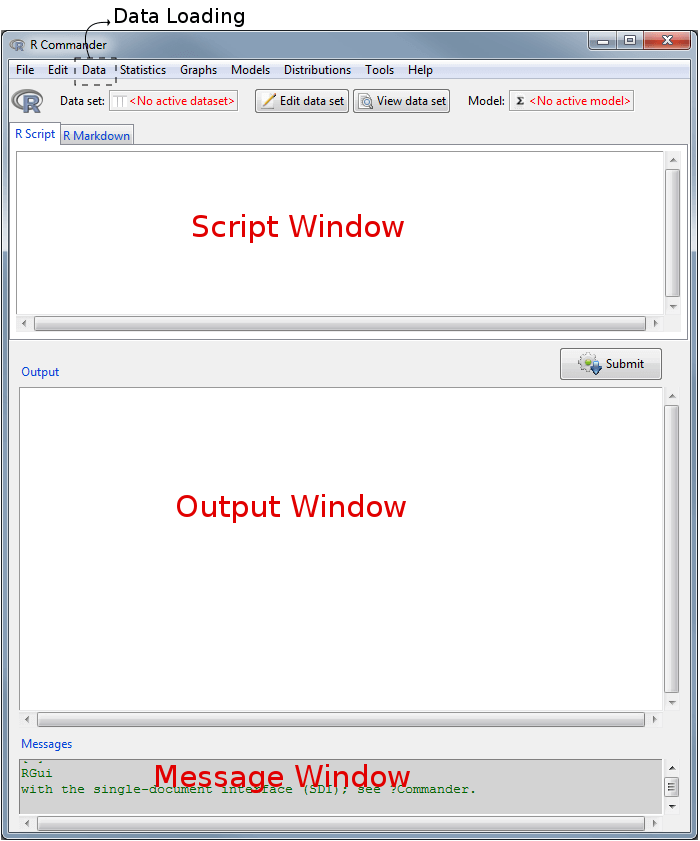
\includegraphics[scale=0.4]{figures/rcmdrwindow.png}
\caption{{\it Default R Commander}\label{rcmdrwindow}}
\end{figure}


%talk about tcltk

% benefits, why rcmdr:
% - point & click for users (extra layer between program &...)
% - see code (learning + reproducing)
% - easy plugin implementation

\subsection{Biclustering}
Let {\bf Y} be a $m \times n$ matrix. The goal of {\it biclustering} now is to
find subgroups of rows and columns which are as similar as possible to each
other and as different as possible to the rest \citep{Kaiser2008}. This
basically comes down to clustering on both the row and column dimension
simultanously and while clustering methods on 1 dimension derive a {\it global
model}, biclustering algorithms will produce a {\it local model}.
For example in clustering algorithms each row in a rowcluster is defined over
all the columns, however a row in a bicluster is selected using only a subset of
columns.\\
Going back to the matrix {\bf Y}, this corresponds to looking for submatrices
with a high similarity of elements. This submatrix is what is called a {\it
bicluster}.
$$
Y = 
\begin{pmatrix}
  a_{11} & a_{12} & \cdots & a_{1n} \\
  a_{21} & a_{22} & \cdots & a_{2n} \\
  \vdots  & \vdots  & \ddots & \vdots  \\
  a_{m1} & a_{m2} & \cdots & a_{mn}
\end{pmatrix}
$$
\noindent While biclustering has its applications in many areas such as
marketing and behavior science, a popular use of it is for the analysis of
genetic data. The {\bf Y} matrix would then be a gene expression matrix in which the
rows correspond with the genes and the columns with the conditions/samples. In
this setting $a_{mn}$ is the expression level of the $m$th gene under the $n$th
condition and biclustering algorithms will identify groups of genes that show
similar activity patterns under a specific subset of the conditions. Therefore,
biclustering is the key technique in situations where a cellular process, in
which only a small set of the genes participate, is of interest or in the
situation that an interesting cellular process is active only in a subset of the
conditions. 
\\ \\
There exist a great deal of different biclustering algorithms today and several
authors have provided extensive reviews, discussion and comparisons of these
(\citealp{Madeira2004}, \citealp{Tanay2004} and \citealp{Prelic2006})\\
All these different algorithms are able to identify several types of
biclusters which can be identified into four major classes:
\begin{enumerate}
  \item Biclusters with constant values
  \item Biclusters with constant values on rows or columns
  \item Biclusters with coherent values
  \item Biclusters with coherent evolutions
\end{enumerate}
To briefly elaborate on this, coherent values would mean that each row and
column can be obtained by adding a constant to each of the others or by
multiplying each of the others by a constant value. Further in the evolution
approaches, the elements of the matrix are viewed as symbolic values and
biclusters with coherent behaviour will be discovered regardless of the exact
numeric values in the matrix. These types of biclusters can be found in
Figure \ref{bicluster_types} in the Appendix.\\
It is also interesting to know that while many biclustering algorithms perform
simultaneous clustering on both dimensions of the data matrix, there also exist
two-way clustering approaches. These use one-way clustering to produce clusters
on both dimensions of the data matrix separately.
\\ \\
Finally, if a biclustering algorithm assumes the existence of several
biclusters, several underlying structures of the data matrix can be considered.
\citet{Madeira2004} listed the following eight major types of underlying
bicluster structures:

\begin{enumerate}
  \item Exclusive row and column biclusters (rectangular diagonal blocks after
  row and column reorder).
  \item Non-Overlapping biclusters with checkerboard structure.
  \item Exclusive-rows biclusters.
  \item Exclusive-columns biclusters.
  \item Non-Overlapping biclusters with tree structure.
  \item Non-Overlapping non-exclusive biclusters.
  \item Overlapping biclusters with hierarchical structure.
  \item Arbitrarily positioned overlapping biclusters.
\end{enumerate}
\noindent These different structures are visualized in figure
\ref{bicluster_structures} in the Appendix.
\newpage


\section{Envelope Packages - Software Development using R}
\noindent There exist a great number of packages for R. On CRAN for example
there are almost 6000 packages available which handle many topics. 
Due to the fact that for each topic or area many packages can be installed, it
can sometimes be challenging for new users to quickly execute a certain
analysis of interest (e.g. dose-response modelling, biclustering
methods, etc.).\\
The creation of {\it `envelope packages'}, related to a common data analysis
problem, can be a solution to this often-occuring problem. 
An attractive way to implement this, is with the help of a Graphical User
Interface (= GUI).\\
The idea is to design a joint development programming environment in which
methodological developers can include their packages in this `envelope
package' without too much programming effort.\\
Not only can multiple people contribute to this `envelope package', the users
will be able to make use of all of these packages in one clear environment. 
To clarify, all the implemented packages in the {\it `envelope
package'} are still independent entities on CRAN or Bioconductor. This means the
{\it `envelope'} package is simply depending on these other packages, not
incorporating the actual code behind them. As a result, any updates by the
authors on an outsourced package will also automatically update the {\it
`envelope package'}. The main goal of the {\it `envelope package'} is to provide
a solid and intuitive `module-like' structure in which the external packages can
fit in, while also providing the possibility of interconnecting these packages.
\\ \\
So while the packages are still independently developed, the end user will only
need this `envelope package' to carry out a specific analysis for which multiple
methods exist. The `envelope package' can make sure the output of implemented
packages is processed in a similar way, providing a user-friendly environment to
execute each step of an analysis. An example of this could be that after
applying a certain analysis method, the results can immediately be visualized
through an appropriate button in the GUI. \\ \\
Further, such an `envelope package' also introduces a lot of flexibility in the
way several packages can be connected, providing an easier workflow. For
example a package focused at the visualisation of results could easily be
connected with other packages in a GUI, alleviating the work of the user in
figuring the right data input for each function.\\
Also, by creating the GUI as a plug-in for R-Commander, it will not deny the
user access to the actual R code which is used for applying a certain analysis.
The R-Commander window will generate the actual R code on the fly which can be
saved, re-executed and even edited. Before, in other GUI systems for R, this was
not yet possible. They did not provide any insight for the user about the R code
behind the functionalities.
\\ \\
It is this concept which was the basis for the development of the
\verb|RcmdrPlugin.BiclustGUI| package. The goal of this package is to serve
as a platform from which several biclustering algorithms as well as the
appropriate diagnostics and graphs can be accessed.


%\newpage
%\mbox{}
%\thispagestyle{empty}
\newpage
\section{The BiclustGUI R Package}

\subsection{GUI Structure}
The {\bf general structure} of a biclustering window is always 
the same for each method. This is shown in Figure \ref{def_str}. The
method dialog consists out of two tabs: the {\it biclustering} tab and the {\it
plots \& diagnostics} tab. \\
In the first tab, the user will be able choose the appropriate parameters for a
biclustering algorithm and then click the {\it Show Results} button to execute
it. If relevant, there will also be a small seed box present to set your seed
for this run in order to obtain reproducable results (this will appear as
\verb|set.seed(...)| in the script).
In the second tab, one can find the {\it specific} plots and diagnostic
tools for the chosen method or package. However, from this second tab you are also
able to access more general diagnostics and plots obtained from an external package. Two which are already
implemented are \verb|BcDiag| and \verb|superbiclust|. They can be easily
accessed through a button, provided they are compatible with the chosen method.
Clicking one of these buttons will open up a new window entirely with
additional plotting and diagnostic tools.\\
When these diagnostics are opened up from a specific biclustering window, the
plots and diagnostics will automatically choose the right object to apply their
functions to. This way no extra interference of the user is necessary when applying their
functionality and the user will not have to worry about the communication
between these windows. (See Figure \ref{biclustGUI_struc})
\begin{figure}[H]
\centering
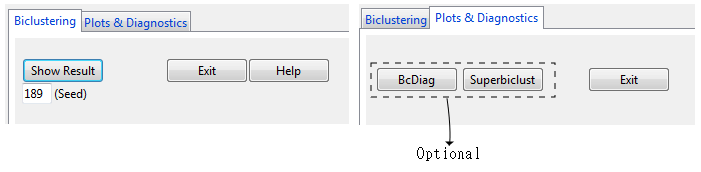
\includegraphics[scale=0.5]{figures/standard_buttons.png}
\caption{{\it Default Window Structure}\label{def_str}}
\end{figure}
\noindent Note that when the graphs are produced they will appear in a separate
graphics device window. Due to the variety of graphical parameters some
diagnostic plots use, it might sometimes be necessary to close this graphics
device down before utilizing a certain graph.(e.g. when you observe the size
of a plot is considerably smaller and multiple are appearing in the same
device). Further, if you would like the save a graph appearing in the device,
simply select the device window and go to the working bar of R itself (not R
Commander). Here, select {\it File}, {\it Save As} and then choose the desired
extension (png, pdf,...).
\\ \\
\noindent Finally, each biclustering method can be accessed from the {\it
Biclustering} menu (see Figure \ref{biclustering_menu}) in R commander which
will appear after loading the plug-in.
\begin{figure}[H]
\centering
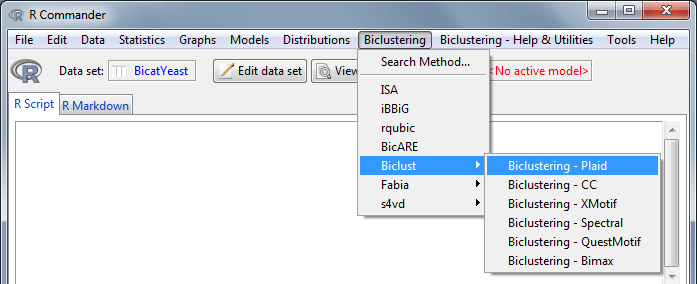
\includegraphics[scale=0.5]{figures/biclustering_menu.png}
\caption{{\it Biclustering Menu (Biclust submenu)}\label{biclustering_menu}}
\end{figure}
\noindent The implemented algorithms and diagnostic tools can be found in Table
\ref{package_table}.

\begin{table}[H]
\centering
\resizebox{\linewidth}{!}{
\begin{tabular}{ccl}
{\bf Type} & {\bf Package} & {\bf Method/Description}\\
\hline
\multirow{22}{*}{{\it Biclustering Algorithms}} &
\multirow{6}{*}{\texttt{biclust}} & Plaid \\
& & CC\\
& & XMotif\\
& & Spectral\\
& & QuestMotif\\
& & Bimax\\
& & \\
& \multirow{4}{*}{\texttt{fabia}} & Laplace Prior\\
& & Post-Projection\\
& & Sparseness Projection\\
& & SPARSE\\
& & \\
& \texttt{isa2} & The Iterative Signature Algorithm\\
& & \\
& \texttt{iBBiG} & Iterative Binary Biclustering of Genesets\\
& & \\
& \texttt{rqubic} & Qualitative Biclustering\\
& & \\
& \texttt{BicARE} & Biclustering Analysis and Results Exploration\\
& & \\
& \multirow{2}{*}{\texttt{s4vd}} & SSVD (Sparse Singular Value Decomposition) \\
& & S4VD (SSVD incorporating stability correction) \\
& & \\
\hline
& & \\
\multirow{3}{*}{{\it General Plots/Diagnostics}} & \texttt{BcDiag} & Bicluster
Diagnostics Plots \\
& & \\
& \texttt{superbiclust} & Generating Robust Biclusters from a Bicluster Set
\end{tabular}
}
\caption{{\it Table of implemented packages}\label{package_table}}
\end{table}
\begin{figure}[H]
\centering
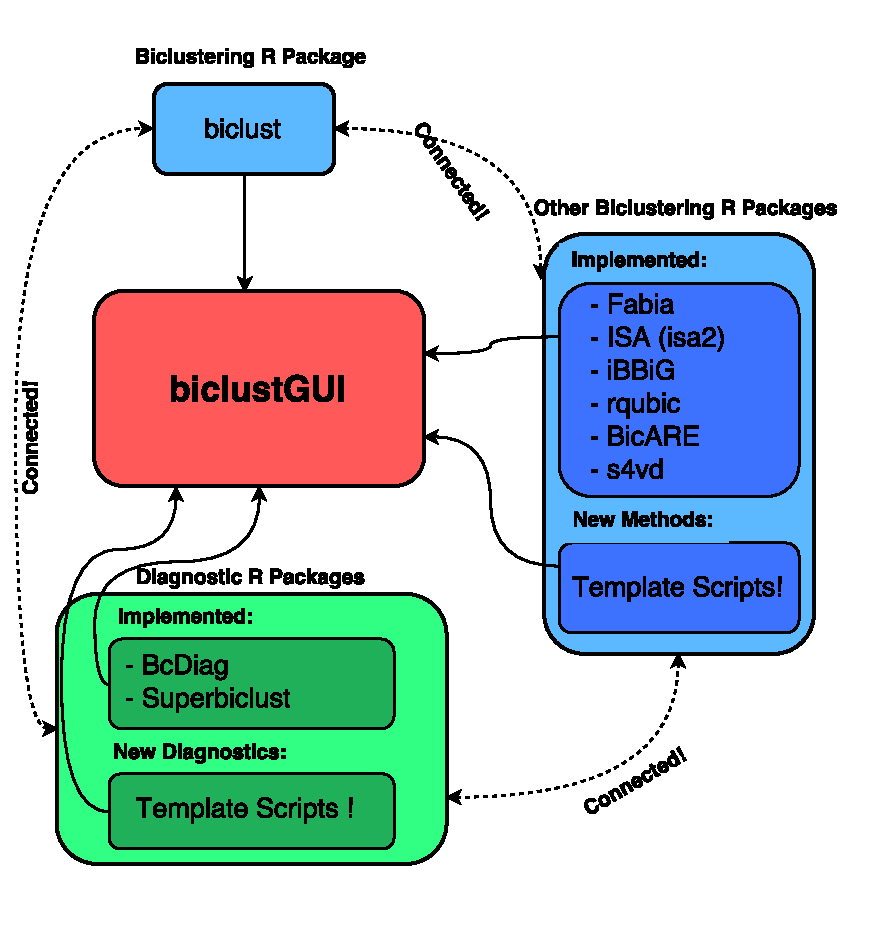
\includegraphics[scale=0.9]{figures/biclustGUI_diagram.pdf}
\caption{{\it The BiclustGUI Structure }\label{biclustGUI_struc}}
\end{figure}

\subsection{Installing and Loading}
\noindent Like a lot of R packages, \texttt{RcmdrPlugin.BiclustGUI} can simply be downloaded
from CRAN at \url{http://cran.r-project.org/web/packages/Rcmdr/index.html} or
simply by using \verb|install.packages| in the R console. \\ \\
Since the BiclustGUI package relies on other biclustering packages, these
should be installed as well. This can be done automatically by setting the
repository to both CRAN and Bioconductor as shown in the panel below:
\begin{verbatim}
setRepositories(ind=c(1:5))
install.packages("RcmdrPlugin.BiclustGUI")
\end{verbatim}

\noindent If there are any installation issues, the dependencies can also be
installed manually as shown in the following panels.
Some of the packages are located on CRAN,
\begin{verbatim}
## PACKAGES AVAILABLE ON CRAN ##
install.packages("biclust")
install.packages("BcDiag")
install.packages("superbiclust")
install.packages("Rcmdr")
install.packages("isa2")
install.packages("s4vd")
install.packages("gplots")
install.packages("viridis")
\end{verbatim}
\noindent while others are available in Bioconductor
\begin{verbatim}
## PACKAGES AVAILABLE ON BIOCONDUCTOR ##
source("http://bioconductor.org/biocLite.R")
biocLite("iBBiG")
biocLite("fabia")
biocLite("rqubic")
biocLite("BicARE")
\end{verbatim}
\noindent Once all R packages are installed we can install the GUI using the following
code. You can either install the development version from the R-Forge repository
or the release version from the CRAN repositiry.
\begin{verbatim}
## Biclust GUI - In Development Version ##
install.packages("RcmdrPlugin.BiclustGUI",
repos="http://R-Forge.R-project.org")
## Biclust GUI - Release Version ##
install.packages("RcmdrPlugin.BiclustGUI")
\end{verbatim}
Note that at first launch the GUI (R Commander) will still prompt to install
some required packages. These can be installed by accepting the request.\\
\noindent After succesfully installing the plug-in, the easiest way to load the
BiclustGUI is by using the command
\begin{verbatim}
library(RcmdrPlugin.BiclustGUI}
\end{verbatim}
in the R console. This will open up the main window of R Commander which can, if
closed, be reopened with the \verb|Commander()| command. \\
\noindent All the commands to install the necessary packages can also be found
in the appendix.

\subsection{Data Input}
There are a couple of ways on how to load data into the \verb|Rcmdr| package
(Figure \ref{datainput}):
\begin{itemize}
  \item Enter {\it new} data directly with: {\it Data $->$ New data set ...}
  \item Load an existing data set from the {\it R workspace}: {\it Data $->$ Load data set ...}
  \item Import existing data from a plain-text file, other statistical packages
  (SPSS, SAS, Minitab, STATA) or even an Excel file: {\it Data $->$ Import data $->$ (choose required option)}
  \item Use a data set which is included in an R package: {\it Data $->$ Data in
  packages $->$ Read data set from an attached package ...}
\end{itemize}
\noindent Once the data is loaded in, it will be the active data set in the form
of a data frame (see Figure \ref{activedataset}). Further note that in most
cases the biclustering procedures require a data matrix with the rows as genes and the columns as conditions/samples.
\begin{figure}[H]
\centering
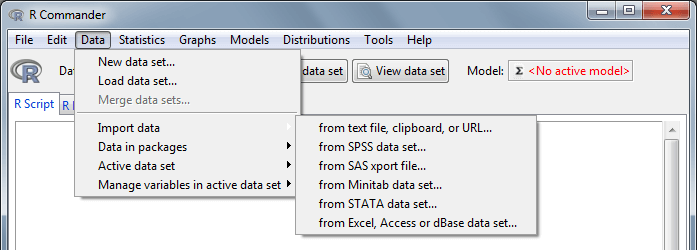
\includegraphics[scale=0.5]{figures/rcmdr_datainput.png}
\caption{{\it R Commander - Data Menu}\label{datainput}}
\end{figure}
\begin{figure}[H]
\centering
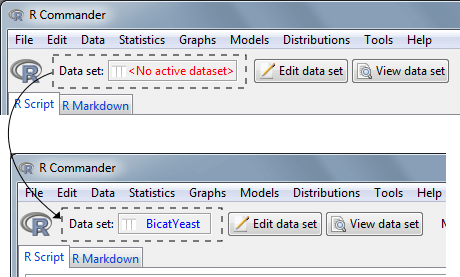
\includegraphics[scale=0.5]{figures/rcmdr_activedataset.png}
\caption{{\it R Commander - Active Dataset}\label{activedataset}}
\end{figure}

\subsection{Extra Utilities}
{\it Note on Active Dataset}\\
Some of utilities also make use of the dataset which was used to obtain a
certain biclustering result (e.g. Exporting Results). If the result was obtained in this
session, the correct dataset will automatically be made the active one.
Otherwise please make sure the correct corresponding dataset is chosen as the
active one in R-Commander.
\subsubsection{Search Dialog}
In the {\it Biclustering} menu, there is also an option called {\it `Search
Method...'}. This option will open up a small window (Figure
\ref{searchwindow}) in which the user can query the available biclustering
methods for several criteria. After the search, one of the methods (which appear
in the list box) can be selected and then opened up with the {\it Go To} button.

\begin{figure}[H]
\centering
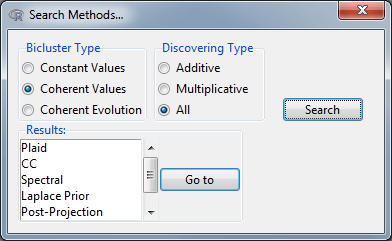
\includegraphics[scale=0.6]{figures/searchwindow.png}
\caption{{\it Search Biclustering Method Dialog }\label{searchwindow}}
\end{figure}

\subsubsection{Help Documentation \& Scripts}
Next to the {\it Biclustering} menu is the {\it Biclustering - Help \&
Utilities} menu (See Figure \ref{biclustering_helpmenu}. The first submenu {\it Help
Documentation} contains three items. The first, {\it Helppage BiclustGUI}, will
lead to the help files of the R package. The next, {\it Vignette BiclustGUI},
will open up the vignette for the BiclustGUI. This document contains information
about the GUI itself as well as a guideline on how to implement new biclustering
methods. The last item, {\it Template Scripts}, will open up the folder in which
these scripts are localised. The developers can use these to create windows for
their own package after which they can send them to the maintainer of the GUI
who can include them in the next update.

\begin{figure}[H]
\centering
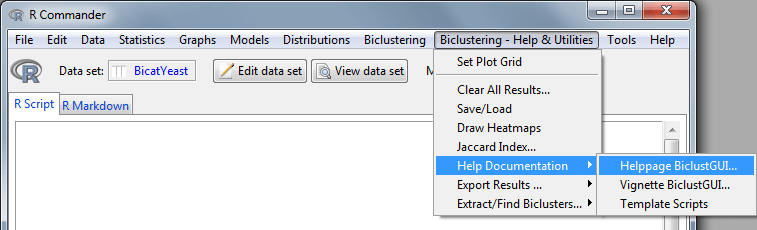
\includegraphics[scale=0.5]{figures/biclustering_helpmenu.png}
\caption{{\it Biclustering Helpmenu }\label{biclustering_helpmenu}}
\end{figure}

\subsubsection{Plot Grid}
\noindent Clicking on this item will bring up a small window (Figure
\ref{plotgridwindow}) from which it is possible to set the grid of the graphics
device in which the plots will be created. This can be helpful in order to show
multiple plots on 1 graphics device. By default this setting is put to 1 by 1
(unless some specific plots require a different grid).
\begin{figure}[H]
\centering
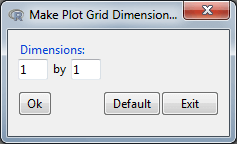
\includegraphics[scale=0.5]{figures/plotgridwindow.png}
\caption{{\it Set Plot Grid Window }\label{plotgridwindow}}
\end{figure}

\noindent {\bf Note: } This option will mostly only work for the graphs which
only contain 1 plot. If some graphs already require an own grid to be set with
multiple plots (e.g. the visualisation of the bootstrap (1 by 2) ), it will not
be compatible with this setting. (A new plot will however follow your own
setting again.)\\
The only exception to this are the graphs from BcDiag which contain multiple
plots. If your grid setting is large enough, they will simply be added into it.
\\
Further, some more advanced grid settings, like for the General Plot for iBBiG,
might require the user to re-apply your own settings.

\subsubsection{Draw Heatmaps}
The next utility is the ability to draw heatmaps of data or biclustering
results. Clicking this button will open up a window which consists out of 2 tabs
as shown in Figure \ref{drawheatmapswindow}. 
\begin{figure}[H]
\centering
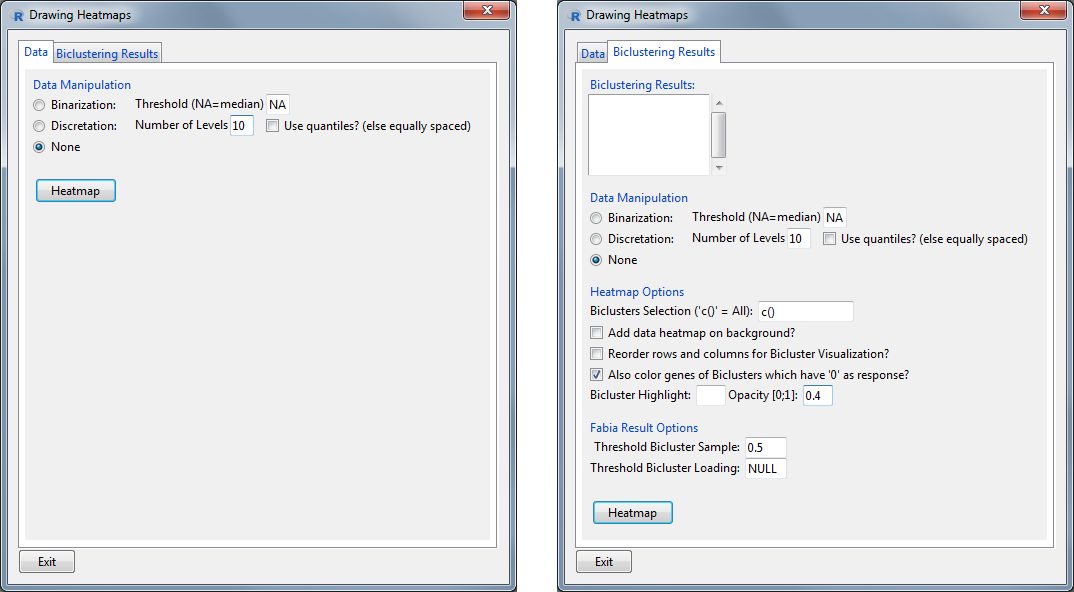
\includegraphics[scale=0.4]{figures/drawheatmapswindow.png}
\caption{{\it Draw Heatmaps Window }\label{drawheatmapswindow}}
\end{figure}

\noindent In the first tab of the window, a heatmap of the Active Dataset can be
plotted. It is also possible, if necessary, to binarize or discretize the data
beforehand. An example of these plots are given in Figure
\ref{drawheatmaps_example1} and \ref{drawheatmaps_example2} in the Appendix.
\\ \\
\noindent The {\it biclustering results} tab provides all the tools to plot the
heatmap of any of the results in the current session. Simply select a result in
the result box and press the {\it Heatmap} button. \\
Further there are also some extra options under the {\it Heatmap Options} title.
If required, only some specific biclusters can be plotted by putting a vector
(e.g. \verb|c(1,2,3)|) in the entry field. Next it is also possible to add the
original data heatmap on the background in a transparent fashion (Again this
background heatmap can be binarized or discretized with the options above).
Also note that if binary data is being used (by default or through the
transformation option), regardless of the fact if the background option is
checked, the heatmap will look slightly different. The difference is that not
all fields are white if they don't belong to a bicluster, they can also be gray.
This simply means that this row and column combination had a '1' response, but
was not included in a bicluster.\\
Next, the following option will reorder the rows and columns of the matrix so
the resulted biclusters are generally put more together. The algorithm to
accomplish this was borrowed from the heatmap plot in the \verb|iBBiG| package.
The next option will determine if row/column combinations in biclusters should
also be colored even if the response was '0'. This is mostly helpfull when investigating binary data if for example you know the resulting biclusters might still
contain zeros (depending on the algorithm). In this case checking this option would show
the full biclusters, but when unchecked, some blocks of the biclusters might
turn white.\\
\noindent Finally, the last option allows the user to highlight 1 single
bicluster. This can be especially helpful after reordering the rows and columns
which results in many overlapping parts. When highlighting the bicluster, it will be brought to
the foreground and all other biclusters will become transparent as given by the
opacity parameter.
\\ \\
Lastly, do take care that it is not possible to visualize overlapping biclusters
that well in these 2D heatmaps. The biclusters are drawn in the order they
appear in the legend so a higher numbered bicluster might be drawn on top of
another (if the biclustering algorithm is able to find such biclusters). Drawing only a
selection of biclusters might be helpfull in this
scenario. Another solution could be to turn to software like FURBY
for which the results can be exported.

\subsubsection{Jaccard Index}
\noindent In the Jaccard Index Window (Figure \ref{jaccardindexwindow}) it is
possible to compute the Jaccard Index between 2 biclustering results which can
be selected in the results box.

\begin{figure}[H]
\centering
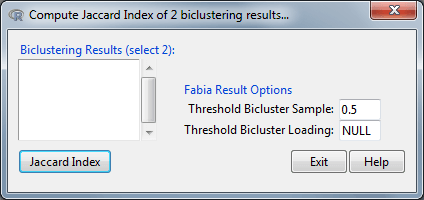
\includegraphics[scale=0.4]{figures/jaccardindexwindow.png}
\caption{{\it Compute Jaccard Index Window }\label{jaccardindexwindow}}
\end{figure}

\subsubsection{Clear Results}
The {\it Clear Results} button in the {\it Help \& Utilities} menu will
automatically clear this session of all biclustering results. This might be
helpfull if one would like to investigate a new dataset.

\subsubsection{Export Results}
Further it is also possible to export the results either as a text file or in
the necessary format for FURBY, Fuzzy Force-Directed Bicluster Visualization (\url{http://caleydo.github.io/projects/furby/}). \\
Note that all the results will appear in the result box. This means that those
result object which are for example manually named by the user will also appear
in the box. Also take care that the correct data set is the active one in R
Commander so that it corresponds with the chosen result (if the result was
obtained in a previous session). the dialogs are shown in Figure
\ref{exportwindows}.

\begin{figure}[H]
\centering
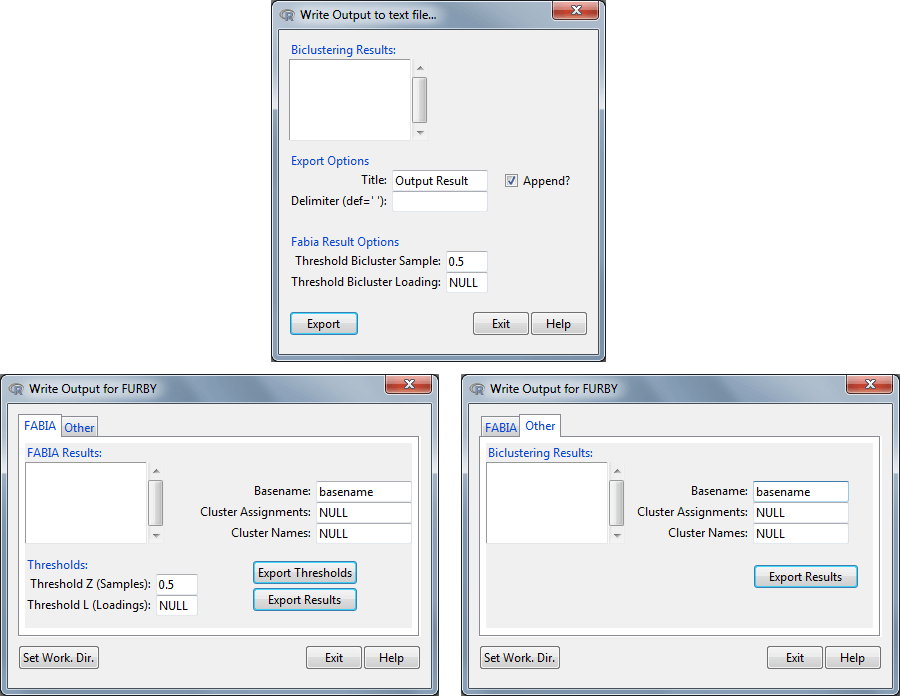
\includegraphics[scale=0.5]{figures/exportwindows.png}
\caption{{\it Export Windows}\label{exportwindows}}
\end{figure}

\subsubsection{Extract Biclusters}
\noindent Another option the user has is to extract the biclustering results in
a list object through the {\it Extract Window} (Figure \ref{extractwindow}). The extracted
object is a list object in which each element is a bicluster (in the form of again a list
object). Each bicluster list element can contain the following items: the
indices of the rows and/or columns in the bicluster and the corresponding names
of these rows and/or columns.
\\ \\
First of all it is also possible to get a quick summary of the selected result
with the {\it Summary} button. Below this button, the options for the actual
extracting are situated. These options include the thresholds for fabia results,
choosing which bicluster to extract and which dimensions to include in the
resulting list object. The user can either choose to extract all biclusters, a
certain range (e.g. from 2 to 6) or a specific selection (in the form of a
vector: e.g. \verb|c(3,6,11)|).\\
Finally, the user can also save the extracted list object in an .rData-object in
the current working directory (which can be changed with the {\it Set Work Dir.}
button). The name for this saved object will be determined by the entry in {\it
Extract Name} (Note that this name also determines the name of the extracted
object in the workspace, even when not saving it).


\begin{figure}[H]
\centering
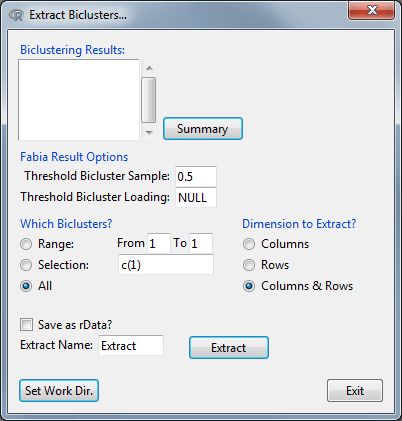
\includegraphics[scale=0.5]{figures/extractwindow.png}
\caption{{\it Extract Window}\label{extractwindow}}
\end{figure}

\subsubsection{Search for genes or samples in biclusters}

\noindent In this window (Figure \ref{findwindow}) it is possible to go through several
biclustering results and investigate if certain rows (= genes) or columns (= samples) are
appearing together in a bicluster. 
\begin{figure}[H]
\centering
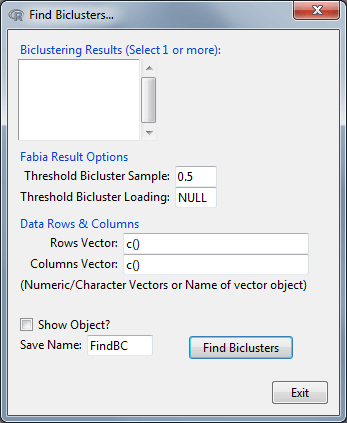
\includegraphics[scale=0.5]{figures/findwindow.png}
\caption{{\it Find Biclusters Window}\label{findwindow}}
\end{figure}
\noindent The way this is done is by simply selecting
one or more of the available results in the list box, setting an optional
threshold for the possible Fabia results (which will then all have the same
threshold) and then simply making vectors containing the rows and/or columns of interest. These
can either be the indices (e.g. \verb|c(1,6,77)|) or the names (e.g.
\verb|c("249364_at","258239_at")|). It is also possible to simple enter the name
of an R object containing such a vector.\\
After this, the user can enter the name in which the result is saved and then
press the {\it Find Biclusters} button. This will execute the function, save the
result and also give a small summary in the console. This small summary contains
the total number of found biclusters and will also show how many biclusters were
found in each result together with which ones they actually are (Figure
\ref{findwindow_example1}).
\\
The saved result is a list object containing the same information as well as
information of the found biclusters itself (in the same format as in the extract
window). The list object also has an element which contains which rows and
columns were chosen to search through the biclusters.
(The {\it Show Object} checkbox simple determines if the result should be
printed afterwards or not.)
\begin{figure}[H]
\centering
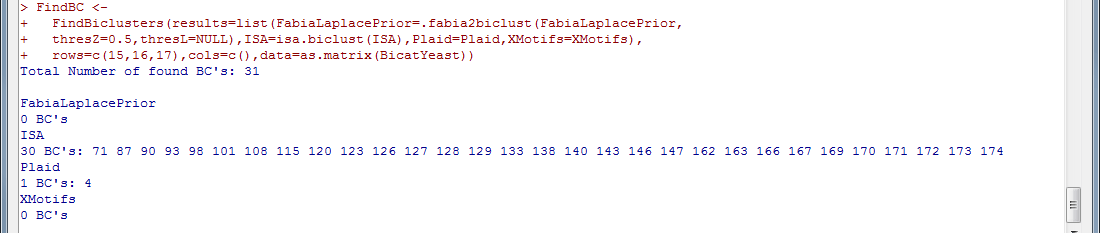
\includegraphics[scale=0.4]{figures/findwindow_example1.png}
\caption{{\it Find Biclusters Summary}\label{findwindow_example1}}
\end{figure}





\subsubsection{Save/Load}\label{sec:SaveLoad}

\noindent Another available option for the user is to {\it Save} a result from a
certain method (as a \verb|RData| or \verb|rda| file) and to also {\it Load} it
back in in a later session.
This is done through the dialogs shown in Figure \ref{saveloadwindow}.
\begin{figure}[H]
\centering
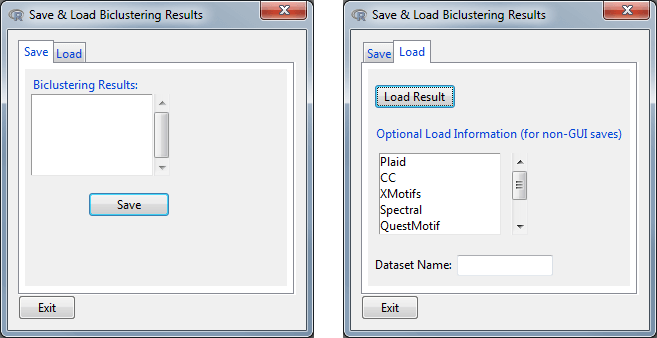
\includegraphics[scale=0.4]{figures/saveloadwindow.png}
\caption{{\it Save \& Load Windows}\label{saveloadwindow}}
\end{figure}
\noindent In the first tab, the user can simply select the desired result and
save it through the {\it Save} button. Note that in this \verb|RData| object also some
info will be stored on what method and which data were used.\\
In the second tab, if the result was saved with the button in the first tab, the
\verb|RData| object can be loaded into the GUI will the {\it Load Result}
button. However if the \verb|RData| object was not created through the save
functionality of the GUI, the additional saved information will not be
automatically available. In this case the user needs to select which method was
used in the list box and fill in the name of the data as well. Please take care
that the name of the object inside the \verb|RData| file has the same name as
the file itself.
\\ \\
{\it Note: Please note that if you are hiding the extensions of known files on your computer, during the save process the \verb|RData| or \verb|rda| extension might not be appended automatically.
You will have to add it manually.}

\subsection{\texttt{biclust}-package}

\subsubsection{Plaid Biclustering}
The plaid biclustering in the GUI implements the plaid algorithm by
\citet{Turner2005} which was proposed as an improvement of the plaid model
discussed by \citet{Lazzeroni2000}. The plaid model is a biclustering method
which takes the interactions between biclusters into consideration by defining
the data structure (e.g. expression level) as a sum of layers. This model
includes a background layer to capture the global effects and afterwards the
method will construct a series of layers that represent the biclusters.
\\ \\
\noindent {\bf Plaid Model:}
\begin{center}
\begin{align}
\displaystyle Y_{mn} = \theta_{mn0}+
\sum_{p=1}^{P}\theta_{mnp}\gamma_{mp}\eta_{np}+\epsilon_{mn} \\
%\\
\vspace{0.3cm}
%$
\gamma_{mp}=\left\{ \begin{array}{ll}  
                     1 & m \in p \\
                     0 & otherwise
                     \end{array}
            \right.
,\text{ and }
\eta_{np}=\left\{ \begin{array}{ll}  
                     1 & n \in p \\
                     0 & otherwise
                     \end{array}
            \right. 
            \\
%$
%\\
\vspace{0.3cm}
%$
\theta_{mnp}=\left\{ \begin{array}{ll}
    \mu_p&\text{(3.1)}\\\mu_p+\alpha_{mp}&\text{(3.2)}\\\mu_p+\beta_{np}&\text{(3.3)}\\\mu_p+\alpha_{mp}+\beta_{np}&\text{(3.4)}
\end{array} \right.
\end{align}
\end{center}
\noindent In (1), $Y_{mn}$ is the expression level of gene $m$ in
condition $n$ with $m=1,\cdots,M$ and $n=1,\cdots,N$. Further, $p$ is the layer
index, $P$ is the number of biclusters, $\theta_{mn0}$ is a sum of overal mean
and $\epsilon_{mn}$ is a random error with mean zero. The model also contains
two indicator variables, $\gamma_{mp}$ and $\eta_{np}$ which represent the the
membership of the gene/condition in a bicluster $p$ as formulated in (2).
Finally $\theta_{mnp}$ is the mean gene expression which can take four possible
forms as shown in (3). In this formula, (3.1) implies a constant bicluster
whereas (3.2) and (3.3) respectively imply biclusters with constant rows or
columns. The last one, (3.4) implies a bicluster with coherent values across the
genes and conditions in a bicluster.
\\ \\
\noindent The estimation of the plaid method is done with an iterative
algorithm. First the background layer is fitted, then the bicluster-specific
layers are added one at a time. In each iteration the algorithm will estimate
the parameters with binary least squares after which a permutation test is
performed which is a built-in protection against the discovery of random
biclusters. This procedure is repeated until no layer is found anymore or until
the maximum amount of layers as been reached. More detailed information about these
steps can be found in \citet{Lazzeroni2000} and \citet{Turner2005}.
\begin{figure}[H]
\centering
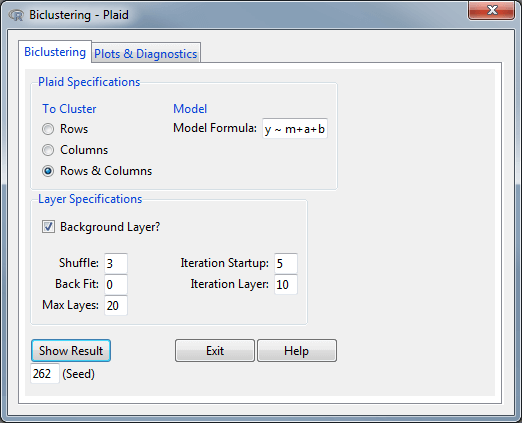
\includegraphics[scale=0.5]{figures/plaid_clusttab.png}
\caption{{\it Plaid Window}\label{plaid_clusttab}}
\end{figure}
\noindent In Figure \ref{plaid_clusttab}, the standard {\it Plaid window} can be
found which contains all the necessary paramaters to apply plaid biclustering. First
the user is able to decide they only want to cluster the rows and columns, or on
both (recommended). Next the model which is fitted to each layer can be
specified in the {\it Model Box}. This coincides with formula (3) and is
defaulted to \texttt{y {\raise.17ex\hbox{$\mathtt{\scriptstyle\sim}$}} m + a +
b} (\verb|m|=constant for all elements in bicluster; \verb|a|=constant for all rows in bicluster; \verb|b|=constant for all columns in
bicluster). 
\\ \\
\noindent The remaining parameters are there to further specify the layer
options in the algorithm. The {\it background} check specifies if there is a
background layer present in the data. {\it Iteration startup} and {\it layer}
define the number of iterations to find respectively the starting values and
each layer. And as already explained earlier, {\it max layers} will determine
the maximum number of layers to include in the model and therefore the maximum
number of biclusters. \\
Finally, {\it Back Fit} specifies the additional iterations to refine the
fitting of the layer and {\it Shuffle} is a parameter connected with the
permutation test. Before a layer is added, its statistical significance is
compared against a number of random obtained layers, defined by this parameter.


\subsubsection{CC($\delta$) Biclustering}
The $\delta$ biclustering, also known as CC algorithm is based on the framework
by \citet{Cheng2000}. The algorithm discovers biclusters one at time and
considers a bicluster as a subset of rows and columns that show coherent values.
The method is a combination of data analysis based on an {\it ANOVA model} and a
{\it node deletion algorithm}.\\
Let $\mathbf{A}_{IJ}$ be a submatrix, i.e. a $\delta$-bicluster, in the data
matrix $\mathbf{A}$ ($I=(i_1,\cdots,i_k);J=(j_1,\cdots,j_k)$). Note that
$a_{ij}$ is the expression leven of gene $i$ in condition $j$.\\
Now Cheng and Church defined a {\it mean residual score} (MSR) as follows
$$
H_{IJ} = \frac{1}{|I||J|} \sum_{i \in I,j \in J}r_{ij}^2
$$
where $r_{ij}=a_{ij}-a_{iJ}-a_{Ij}+a_{IJ},i \in I,j \in J$.\\
A submatrix is now called a bicluster if the MSR is less than a pre-defined
threshold $\delta$.\\
In order to find these $\delta$-biclusters, the algorithm will start with the
full matrix and calculates the MSR. Now the MSR will be minimized by
deleting/including rows and columns in the matrix. Since the {\it brute-force
approach} is computationally not time-efficient, {\it node deletion} algorithms
were developed (single \& multiple) which is a {\it greedy} algorithm. These
algorithms iterate the process of choosing a row and column with the largest MSR
and removing them from the data matrix until the desired submatrix is found.
Note that after the node deletion, the bicluster may not be maximal (some
rows/columns may be added without increasing the MSR) so therefore node
addition is performed by again adding rows and columns one by one (if it does
not increase the MSR).\\
More about both algorithms and the CC biclustering can be found in \citet{Cheng2000}.
\begin{figure}[H]
\centering
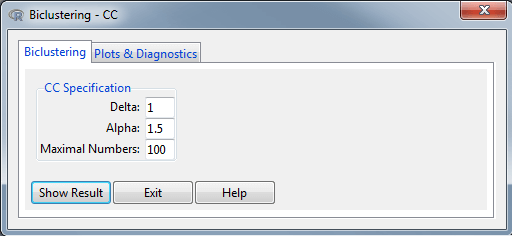
\includegraphics[scale=0.5]{figures/cc_clusttab.png}
\caption{{\it CC Window}\label{cc_clusttab}}
\end{figure}
\noindent As can be seen in Figure \ref{cc_clusttab}, there are not a lot of
input parameters in the {\it CC window} for the $\delta$-biclustering. The most
important parameter is of course {\it Delta}, the maximal accepted score which
will be compared with the MSR. The choice of this variable should depend
on the total variability of the data, taking into account both the assumed
variability of the noise and bicluster values. Next, {\it Alpha} is a scaling
factor. It is a parameter for the multiple node deletion and takes part in the
three major steps of the algorithm:
\begin{enumerate}
  \item Deleting rows and columns with a score larger than {\it Alpha} times the
 matrix score.
 \item Deleting the rows and columns with the largest scores.
 \item Adding rows or columns until {\it Alpha} level is reached.
\end{enumerate}
\noindent Finally, the user is also able to set a maximum number of clusters to
be found with the {\it Maximal Numbers} input parameter. The algorithm will stop
until no bicluster is found or until this threshold is reached.

\subsubsection{XMotifs Biclustering}
The XMotifs biclustering algorithm was proposed by \citet{Murali2003} and
looks for conserved gene expression motifs in a discretized version of the data
matrix. This is achieved by searching for rows with constant values over a set
of columns. The authors assume in their model that the gene can be expressed in
a finite number of states (e.g. 2 states: up- and downregulated). The states of
the gene expression matrix can also be defined by a fold change, represented by
quantile discretization of the original matrix with log-transformed values. A
conserved gene expression motif is now defined as a submatrix of {\it maximum
size} for which the values within each row are equal to the same level. \\
Following the discretization, the biclusters are discovered with an iterative
procedure which will be briefly touched upon down below while explaining the
input parameters of the window. More detailed information can be
found in \citet{Murali2003}.
\begin{figure}[H]
\centering
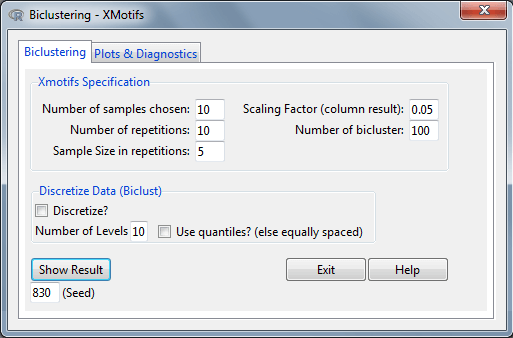
\includegraphics[scale=0.5]{figures/xmotif_clusttab.png}
\caption{{\it XMotifs Window}\label{xmotif_clusttab}}
\end{figure}
\noindent In Figure \ref{xmotif_clusttab}, the {\it Xmotifs window} is displayed
which contains all the necessary input parameters for the algorithm. Note that
in the bottom box, the user is able to discretize the active data set in the R
commander session if necessary. This is done with the \verb|discretize| function
in the \verb|biclust| package. For plotting however, the original matrix will be
used.\\
After the discretization, the algorithm first needs a number of
samples/columns (= {\it `Number of samples chosen'}) to be randomly selected as
a seed. Then a number of sets of samples (= {\it `Number of repetitions'}) of
a defined size (= {\it `Sample size in repetitions'}) needs to be inputted which
will be randomly selected from the samples that were not in the {\it number of
samples chosen}.\\
After this is done, the following steps are performed as described in
\citet{Kaiser2008}:
\begin{enumerate}
  \item Choose a subset from these columns and collect all rows with equal state
  in this subset.
  \item Collect all columns where these rows have the same state.
  \item Return the bicluster if it has the most rows from all found and is also
  larger than a $\alpha$ (= {\it `Scaling factor'}) fraction of the data.
\end{enumerate}
\noindent To collect more than one bicluster, the calculation is rerun without
the rows and columns already found (or return the smaller combinations found). This
is done until the maximum number of biclusters (= {\it `Number of biclusters'})
is achieved or until no clusters can be found anymore.

\subsubsection{Spectral Biclustering}
Spectral biclustering is a method developed by \citet{Kluger2003}, used
for discovering multiplicative biclusters of coherent values. First of all it
assumes that the gene expression matrix assumes a checkerboard structure after
normalization therefore resulting in non-overlapping biclusters. These
biclusters are called multiplicative because each bicluster element ($a_{ij}$, expression level
gene $i$, condition $j$) can be defined as a product of three terms: overall
mean ($\mu$), row-specific ($\alpha_i$) and column-specific ($\beta_j$) means
($\alpha_{ij}=\mu \times \alpha_i \times \beta_j$).\\
The spectral biclustering is mostly based on a singular value decomposition
(SVD) of the normalized data matrix and consists out of the following steps
\citet{Kaiser2008}:
\begin{enumerate}
  \item Re-order the data matrix and apply one of the three normalization
  methods (independent rescaling, bistochastization or log-interactions).
  \item Obtaining eigenvalues and eigenvectors using SVD.
  \item Depending on the normalization method, the biclusters are constructed
  beginning from the largest or second largest eigenvalue. The eigenvectors
  (left \& right) corresponding to the largest eigenvalues are expected to
  provide optimal clustering of rows and columns.
  \item The data is projected on the the best two or three eigenvectors and
  $k$-means clustering is run to get the grouping.
\end{enumerate}
\noindent More detailed descriptions of the above steps can be read in \citet{Kluger2003}.
\begin{figure}[H]
\centering
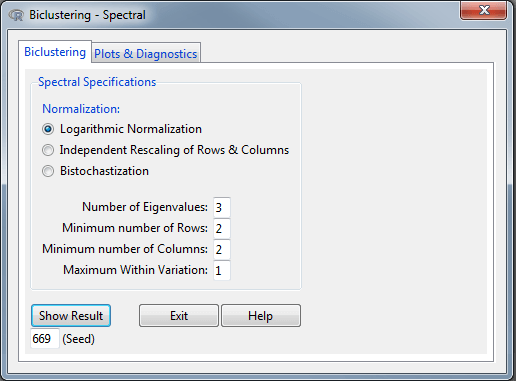
\includegraphics[scale=0.5]{figures/spectral_clusttab.png}
\caption{{\it Spectral Window}\label{spectral_clusttab}}
\end{figure}
\noindent In Figure \ref{spectral_clusttab} above, the {\it Spectral window} is
shown which contains the major steps of the spectral biclustering, namely the
normalization and the SVD. \\
As already explained earlier, the data matrix need to be normalized first as
this is necessary for a checkboard structure to be discovered by the use of
Singular Value Decomposition. The user is able to choose out of three different
options for this step. The {\it Independent Rescaling of Rows \& Columns}
assumes the non-normalized matrix is obtained by multiplying each row and column
with a scalar. {\it Bistochastization} works by repeating the independent
scaling of rows and columns until stability is reached. For this normalization,
the final matrix has all rows sum to a constant and all columns sum to a
different constant. The final method, {\it Logarithmic Normalization} (=
log-interactions) assumes that after taking the logarithm, the original
rows/columns differ by additive constants. Further each row and column is
expected to have mean zero which is achieved with a transformation.
\\ \\
Finally, the user will have to specify the input parameters connected with the
SVD. These include: {\it Number of Eigenvalues}, {\it Minimum number of Rows},
{\it Minimum number of columns}, {\it Maximum Within Variation}. Note the number
of eigenvalues coincides with the number of biclusters that should be
discovered.

\subsubsection{QuestMotif Biclustering}
The Questmotif Biclustering is based on the framework by \citet{Murali2003} and
developed by \citet{Kaiser2011}. The algorithm will search for biclusters of
questioners which have similar answer to the questions.\ \\ \\
\noindent Following now is a short description of the algorithm with respect to
the {\it Questmotif window} in Figure \ref{questmotif_clusttab}.
\begin{figure}[H]
\centering
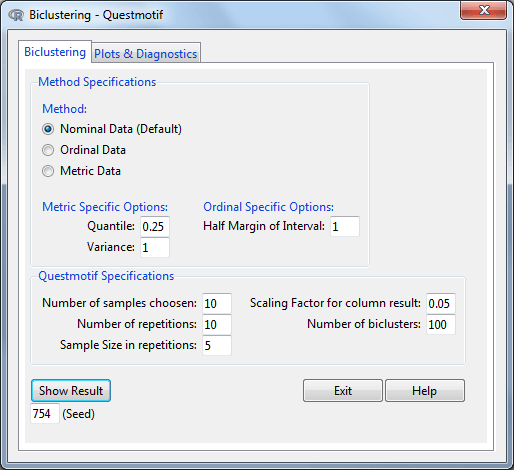
\includegraphics[scale=0.5]{figures/questmotif_clusttab.png}
\caption{{\it QuestMotif Window}\label{questmotif_clusttab}}
\end{figure}
\noindent The Quest algorithm contains three methods to deal with different
scale levels data, especially for biclustering questionnaire data. All of the
three methods can be selected by the user and depending on the choise, some
additional parameters might have to be defined.\\
If the answers are given on a {\it nominal scale}, the algorithm simply works
like the Xmotifs algorithm. For the {\it ordinal scale}, the algorithm will search for
similar answers in an interval of a size set by the parameter {\it `Half Margin
of Interval'} ($=d$). This implies that the interval will be of the form
$[mean-d,mean+d]$. In the continuous case, namely {\it metric data}, this
interval is set by the quantile of a chosen distribution. It uses all previously
found values to calculate the mean value and uses a given parameter for the
variance of this distribution. Both the {\it Quantile} and {\it Variance} will
have to be provided by the user in this case. (Since the normal scores are used
in such data, the normal distribution is commonly used in this case.)
\\ \\
Finally, a couple of general input parameters, used by the algorithm, will have
to be set by user in the {\it Questmotif Specifications} box. These include:
{\it number of samples choosen}, {\it number of repetitions}, {\it sample size
in repetitions}, {\it scaling factor for column result} and {\it number of
biclusters}. Note that these are the same input parameters used by the Xmotif
algorithm.
\\ \\
More insight and details about the algorithm itself can be found in \citet{Kaiser2011}.

\subsubsection{Bimax Biclustering}
The last implemented biclustering method from the \verb|biclust| package is the
{\it Bimax} (= binary inclusion-maximal) biclustering algorithm which was developed
by \citet{Prelic2006}. They advocated its use as a preprocessing step
to identify potentially relevant biclusters that can be used as input for other
methods. According to the authors, the main benefit of the method is the
relatively small computation time while still providing relevant biclusters
using a simple data model. \\
The Bimax algorithm works on a binarized data matrix in which the expression
value is set to 1 if there is a change with respect to the control setting and
to 0 otherwise. If a control setting is unavailable, one can simply take a
threshold based on the distribution of the data values. The goal of the Bimax
method is to find maximal inclusion biclusters. This means a Bimax bicluster
spans a submatrix of 1's which cannot be part of a larger submatrix of 1's. The
algorithm achieves this by applying a divide-and-conquer strategy in which the
rows and columns are rearranged (to concentrate ones in the upper right corner
of the matrix) before dividing the matrix into two submatrices.\\
More detailed information about the algorithm can be found in \citet{Prelic2006}. 
\begin{figure}[H]
\centering
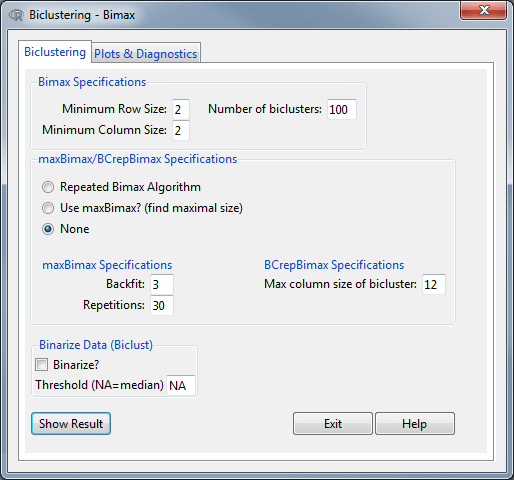
\includegraphics[scale=0.5]{figures/bimax_clusttab.png}
\caption{{\it Bimax Window}\label{bimax_clusttab}}
\end{figure}
\noindent The first box in the {\it Bimax window}, shown in figure
\ref{bimax_clusttab}, are general input parameters required by the algorithm.
These include the {\it minimum row \& column size} of a bicluster (for it to be
included) and the {\it number of biclusters}. The algorithm will terminate when
this boundary level of number of biclusters is achieved or when no more maximal
inclusion biclusters can be found.
\\ \\
Further, \citet{Kaiser2008} suggested that in order to get satisfying
results. the method should be iterated several times with different starting
points. This can be accomplished with the {\it `Use maxBimax'} option in the
second box for which the {\it number of repetitions} and {\it backfit} should be
defined. With this option biclusters of maximal size will be discovered.\\
Finally, also the {\it Repeated Bimax Algorithm} is implemented in this window
for which the {\it max column size of biclusters} should be inputted. More
information about this last variation of Bimax can be found in
\citet{Dolnicar2011}.
\\ \\
Finally in the last box, the active data set in your R Commander session can be
binarized if this is not a binary matrix by default. This is done through a
available function \verb|binarize| in the \verb|biclust| package. A threshold
can be set for this transformation or it can be left on the default option,
namely the median. Do note that when plotting graphs (e.g. the biclust plots),
the original data matrix will be used which is the active data set in your session.



\subsubsection{Biclust: Plots \& Diagnostics}\label{sec:biclustplots}
After executing any of the biclustering methods available in the
\verb|biclust| package, the user is now able to proceed to the second tab {\it
`Plots \& Diagnostics'} which is identical for all of these methods.
No additional work is needed by the user for the plotting and diagnostic
functions to use the correct results from the method which was applied in the
first tab. An example (for the Plaid Biclustering) of the {\it Plots \&
Diagnostics window} is given in Figure \ref{biclust_plotdiagtab}.
Note that the second window in this figure is accessible through the {\it Extra
Biclust Plots} button.
\begin{figure}[H]
\centering
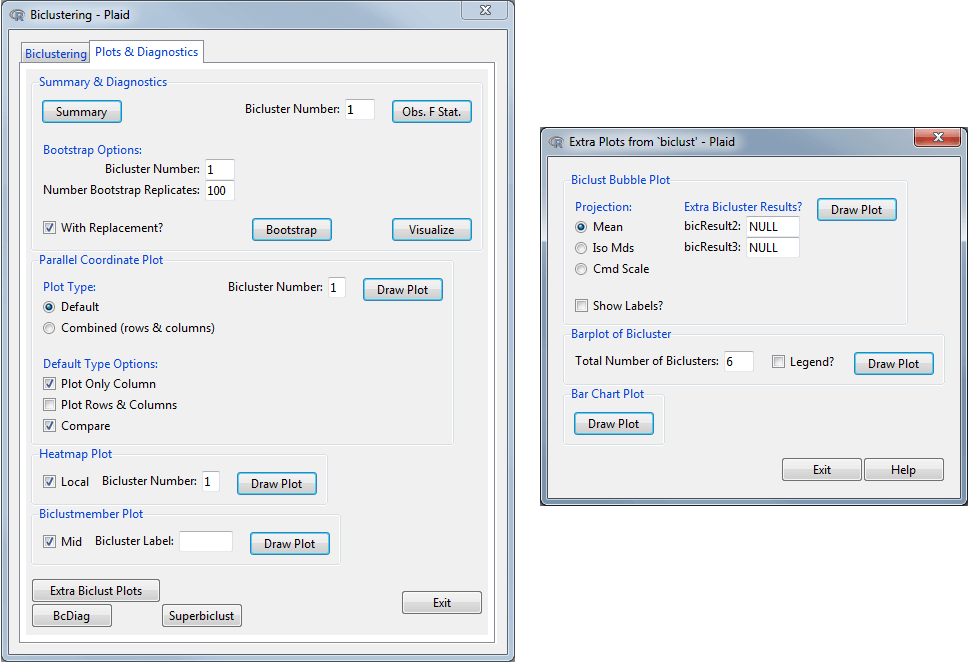
\includegraphics[scale=0.45]{figures/biclust_plotdiagtab.png}
\caption{{\it Biclust - Plots \& Diagnostics Tab}\label{biclust_plotdiagtab}}
\end{figure}
\noindent {\bf Summary \& Diagnostics}\\
\noindent In the first box, the summary of the biclustering result as well as
some basic diagnostics can be called by the user. The {\it Summary} button will
provide the user with the number of clusters found as well with the number of
rows and columns each bicluster contains. Next, the {\it Obs. F Stat.} button
will enable the user to compute some F-statistics about a specific bicluster,
defined by the number in the {\it Bicluster Number} entry box. These
F-statistics include the main effects, namely the row and column, and also the interaction
effect. The first two F-statistics (main effects) are calculated from a two-way
ANOVA with such row and column effect. Because the full model with interaction
is unidentifiable, Tukey's test for non-additivity is used to detect an
interaction within a bicluster. Lastly, the p-values are obtained from
asymptotic F distributions.\\
The last option in this first box, is the ability to calculate p-values of
earlier F-statistics but now with the help of bootstrapping. This means the
p-values are now calculated by taking the number of bootstrap replicates which
are larger than the observed F-statistics and divide it by the total number of
replicates plus one. This number can be set by the {\it Number Bootstrap
Replicates} entry box and the user can also decide to bootstrap with or without
replacement with the corresponding checkbox. The bootstrapping on the defined
{\it Bicluster Number} is executed through the {\it Bootstrap} button after
which the user can use the {\it Visualize} button to obtain histograms of the
bootstrap results of the row and column tests. An example of this graph (and
bootstrapping output) can be found in the Appendix in figure
\ref{biclustplot_example1}. Note that the vertical green line represents the
observed F-statistic.
%(without replacement is actually a permutation test)
\\ \\
\noindent {\bf Parallel Coordinate Plot}\\
\noindent In the next box the user is able to produce a variety of parallel
coordinate plot. The graphs make use of the expression levels in the original
data matrix (unaffected by discretization or binarization). The plot represents
these levels through gene and/or condition profiles in a bicluster as lines.
The bicluster which will be drawn is once again defined by a {\it Bicluster
Number} entry box.\\
The first {\it Plot Type} is the default one for which extra options are
available in the form of checkboxes. By checking only the {\it Plot Only
Column}, the expression levels for the columns in the selected bicluster will be
drawn. This means each line is a column profile with the genes on the x-axis. By
checking {\it Plot Rows \& Columns} a second plot will be added to the graphics
device, but now with the row/gene profiles with the columns/conditions on the
x-axis. The last checkbox, {\it Compare}, will make sure the other profiles, not
in the chosen bicluster, are also plotted in a light-gray colour.\\
Finally the second type, {\it Combined (rows \& columns)}, in a way combines the
information about the bicluster grouping of rows and columns. Again, each line
is a gene/row profile, but the columns/conditions on the x-axis are reordered in
such a way that the columns belonging to the bicluster come first. This is
visualized by showing a red line when belonging to the selected bicluster and
black one when not.\\
An example of these parallel coordinate plots (or profile plots), can be found
in the Appendix in Figure \ref{biclustplot_example2}.
\\ \\
\noindent {\bf Heatmap Plot}\\
In this box, the user can visualize the gene expression data matrix as a
heatmap. The rows and columns will be reordered so that the inputted bicluster
in the {\it Bicluster Number} entry box will appear in the top-left of the
matrix.
However, by checking the {\it Local} option, only the heatmap of the bicluster
will be drawn, omitting the rest of the matrix.\\
An example is given in the Appendix in Figure \ref{biclustplot_example3}.
\\ \\
\noindent {\bf Biclustmember Plot}\\
\noindent The last box on this window contains the options to draw a
Biclustmember Plot. This plot can primarily be used to compare the discovered
biclusters against each other. On this graph, as given in the Appendix in figure
\ref{biclustplot_example4}, one can find multiple columns of stacked rectangles.
Each such column is a representation of a bicluster and each rectangle inside
represents a column/condition/sample of the data matrix. Basically if in a
column of of these stacked rectangles, a rectangle is coloured, it means that
this condition is part of that particular bicluster. Now, if the {\it Mid} box
is not checked, a coloured rectangle consists out of two parts, left and right.
The left colour represents the mean of this condition for all the genes within
the biclusters. However, the right colour contains the global mean value for
this condition. If the {\it Mid} option is checked though, the rectangle exist out of
three colours with the global mean in the middle and the bicluster mean on the
left and right.\\
Finally, the user is also able to set a label which will come in front of the
cluster number with the {\it Bicluster Label} entry box.
\\ \\
\noindent {\bf Biclust Bubble Plot}\\
\noindent The first plot the user can create from the extra window, is the
Biclust Bubble Plot. The bubbleplot is a 2D-projection of the biclusters, done
through multidimensional scaling based on the gene and condition profiles. It is
used as a tool to help understand the overall behaviour of biclustering methods, detect trends, outliers, etc. Each
bicluster is represented as a circle of which the brightness represents the
homogeneity (darker, less homogeneous). The size on the other hand represents
the size of the biclusters, as rows $\times$ columns. The user is able to add up
to three bicluster results in the {\it Extra Bicluster Results} entry boxes,
obtained from earlier runs of methods from \verb|biclust|. Note that each bicluster set
will get a different colour in the plot.\\
Further, the user is also able to choose between three different kind of
projections, namely {\it mean}, {\it Iso Mds} and {\it CmdScale} of which more
information can be found in the help files (note that this {\it Help} button is
linked to the bubbleplot help page). \\
Lastly the {\it Show Labels} checkbox will give each bicluster the corresponding
bicluster number if checked. An example of this type of graph can be found in
the Appendix in Figure \ref{biclustplot_example5}.
\\ \\
\noindent {\bf Barplot of Bicluster}\\
\noindent The graph available in this box is a barplot of biclusters which is
used to compare the values inside a bicluster with the values outside of the
bicluster. For each bicluster, three bars are drawn per column/condition part of
the bicluster. The darkest represents the values inside of the bicluster and the
other two the mean and median of the values outside of the cluster. The user is
able to draw a legend yes or no with the {\it Legend} checkbox and can also
determine the number of biclusters which should be drawn with the {\it Total
Number of Biclusters} entry box. However this works in a slightly different way,
namely on each graphics output device, only 6 bicluster barplots can fit.
Further the spot such barplot will get on this `grid' will always be the same.
For example, if you would take as input the number 14, only bicluster 13 and
14 would appear on the device. If you you would put in the number 12, bicluster
7 to 12 would appear.\\
An example is given in the Appendix in Figure \ref{biclustplot_example6}.
\\ \\
\noindent {\bf Bar Chart Plot}\\
\noindent The final graph in this window will create a barchart for all the
biclusters, representing the columns. Each block represents one bicluster and
the bars inside of it represent the means of bicluster values for the corresponding
column.\\
An example of this is also given in the Appendix in figure
\ref{biclustplot_example7}.

\subsection{\texttt{fabia}-package}
The biclustering algorithm FABIA or Factor Analysis for Bicluster Acquisition
was proposed by \citet{Hochreiter2010}. A couple of variations are
available in the \verb|fabia| packages of which the {\it Laplace Prior}, {\it
Post-Projection}, {\it Sparseness Projection} and {\it SPARSE} are implemented
in the GUI. \\
The main description of fabia will be given for the Laplace prior
implementation. For the others, the differences between the windows will be
briefly touched upon. 
% others, differences windows touched upon
% put general info here
\subsubsection{Laplace Prior}
Factor Analysis for Bicluster Acquisition with Laplace Prior is an algorithm is
based on factor analysis where the homogeneity is based on the latent
relationship between the variables in the data. The method will discover
multiplicative biclusters which are found by sparse factor analysis where both
the factors and loadings are sparse. This assumption of sparseness comes from
the gene expression data, where normally only a small fraction of the genes is
active under a small subset of conditions \citep{Khamiakova2013}. Further, the
model assumes non-Gaussian signal distributions with heavy tails.\\
Now, a factor model for data matrix $Y$ with $P$ factors can be described as
follows
$$
\mathbf{Y}= \sum_{p=1}^P \lambda_p Z_p + \epsilon 
$$
where $Z_p$ is the $p$th factor, $\lambda_p$ is the vector of factor loadings
for $Z_p$ and where additive random noise is assumed to be normally distributed, 
$\epsilon \sim N(0,\boldsymbol\Psi)$. Furthermore, the model assumes that
$\boldsymbol\Psi$ is a diagonal matrix, i.e. the error terms $\epsilon$ are
independently and normally distributed given the $p$ factors in the model.
Another assumption is that $\mathbf{Z}$ and $\boldsymbol\Psi$ are independent
which implies that the noise is independent of the signal strength. Lastly,
as said before, the factor model assumes sparseness of factors and their
loadings and this is reflected by the choice of the corresponding prior on
loadings and factors (i.e. a Laplace Distribution).\\
Using this factor model, biclusters can be be obtained as following. On a
side note, it is important to mention that the method requires normalized and
centered data.
Now, the algorithm will estimate the parameters and factors through maximizing
the posterior of $\boldsymbol\lambda$, $\boldsymbol\Psi$ and $\mathbf{Z}$ with
the help of a variational EM algorithm.
Using the estimates for $\boldsymbol\Lambda$ and $\mathbf{Z}$, the denoized data is
obtained and the biclusters are derived from $\lambda_p Z_p$. This means that
this component can be seen as a bicluster of which the non-zero genes and
samples are members of the bicluster. \\
More intricate details and information about the method and its variations, can
be found in \citet{Hochreiter2010} and \citet{Hochreiter2014a}.
\\ \\
The {\it Fabia with Laplace Prior window} is shown in figure
\ref{fabialaplace_clusttab} in which the fabia specifications as well as some
data manipulation can be decided upon.
\begin{figure}[H]
\centering
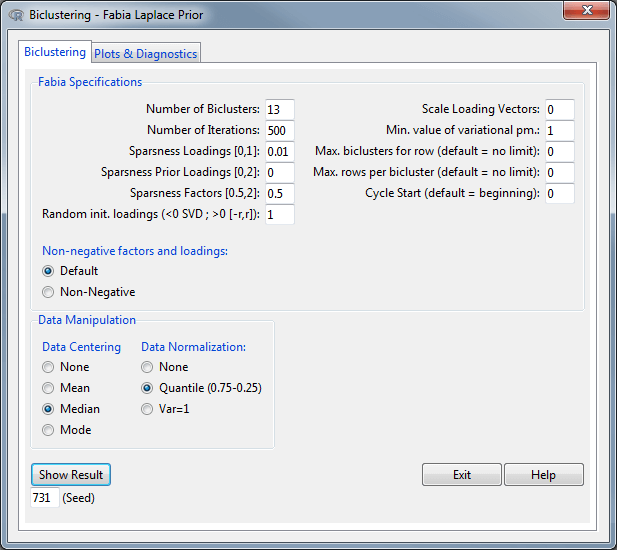
\includegraphics[scale=0.5]{figures/fabialaplace_clusttab.png}
\caption{{\it FABIA (Laplace Prior) Window - Clustering
Tab}\label{fabialaplace_clusttab}}
\end{figure}
\noindent As one can see there are a lot of input parameters which can be
specified. The most important ones are the {\it Number of Biclusters} which is
equal to the number of factors and can be set to the upper boundary. The other
parameters of importance are responsible for the specification of the sparseness
such as the {\it Loadings}, {\it Prior Loadings}, {\it Factors}, etc. These
depend on the noise level in the data and also the size of the data set.\\
The user can also select if the factors and loadings are non-negative
or not. 
\\ \\
Finally, the user can also apply some data manipulation before the method is
executed, namely {\it Centering} and {\it Normalizing} the data matrix.


\subsubsection{Post-Projection}
For {\it Fabia Post-Projection}, some post-processing is present. Namely
the final results of the loadings and the factors are projected to a sparse
vector according to \citet{Hoyer2004}. This means: given an $l_1$-norm and an
$l_2$-norm, minimize the Euclidean distance to the original
vector (currently the $l_2$-norm is fixed to 1).\\
The {\it Fabia Post-Projection window} is given in figure
\ref{fabiapostproj_clusttab}.
\begin{figure}[H]
\centering
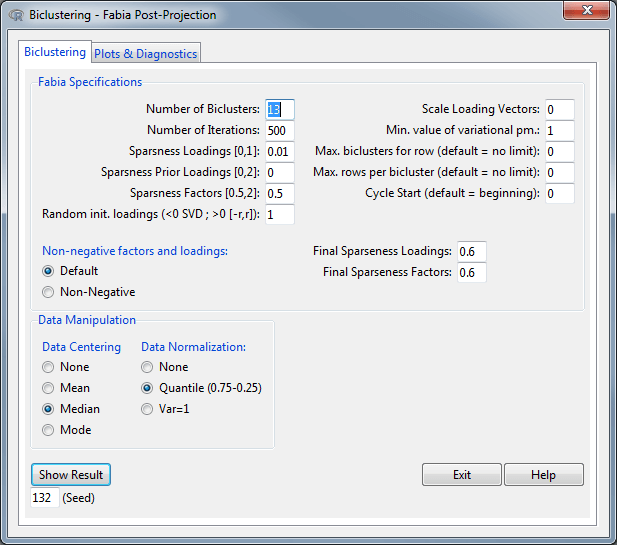
\includegraphics[scale=0.5]{figures/fabiapostproj_clusttab.png}
\caption{{\it FABIA (Post-Projection) Window - Clustering
Tab}\label{fabiapostproj_clusttab}}
\end{figure}
\noindent As one can see, the window is primarily the same as the {\it Laplace
Prior} one, but the user can now also define the {\it Final Sparseness
Loadings} and {\it Final Sparseness Factors}.

\subsubsection{Sparseness Projection}
The next implemented fabia algorithm is fabia with {\it Sparseness Projection}.
In this version, the prior has finite support, therefore after each update of the
loadings they are projected to this finite support. This projection is again
done according to \citet{Hoyer2004} (See {\it Post-Projection}).\\
Figure \ref{fabiasparseproj_clusttab} shows the {\it Fabia Sparseness Projection
window}.
\begin{figure}[H]
\centering
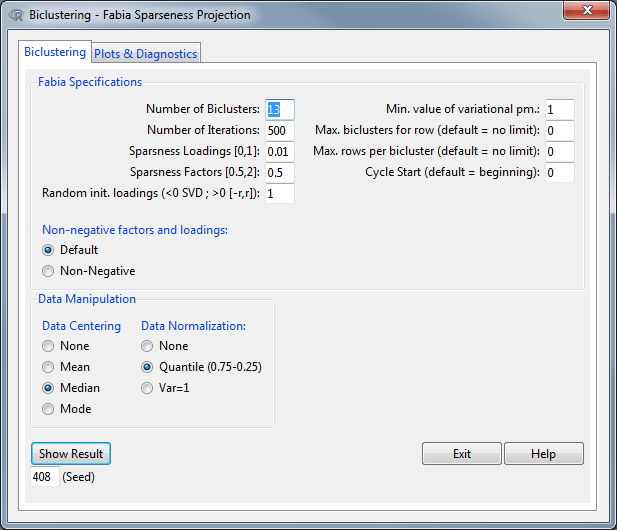
\includegraphics[scale=0.5]{figures/fabiasparseproj_clusttab.png}
\caption{{\it FABIA (Sparseness Projection) Window - Clustering
Tab}\label{fabiasparseproj_clusttab}}
\end{figure}
\noindent The only difference with {\it Laplace Prior} is that some options in
the specifications have disappeared. These include the {\it Sparseness Prior
Loadings} and the {\it Scale Loading Vectors}.
\subsubsection{SPARSE}
This is a version of fabia for a sparse data matrix. The matrix is directly
scanned by C-code and therefore must be in sparse matrix format as described in
\citet{Hochreiter2010} and \citet{Hochreiter2014a}. \\
Again biclusters are discovered through sparse factor analysis and the model
selection is performed by a variational approach according to
\citet{Girolami2001} and \citet{Palmer2006}. Further a prior on the parameters
is included and a lower bound on the posterior of the parameters is minimized, given the data. The
update of the loadings includes an additive term which pushes the loadings
towards zero (Gaussian prior leads to a multiplicate factor).\\
More detailed information about this algorithm and its methodology can be
found in \citet{Hochreiter2010} and \citet{Hochreiter2014a}. The {\it Fabia
SPARSE window} is shown in Figure \ref{fabia_sparse}.
\begin{figure}[H]
\centering
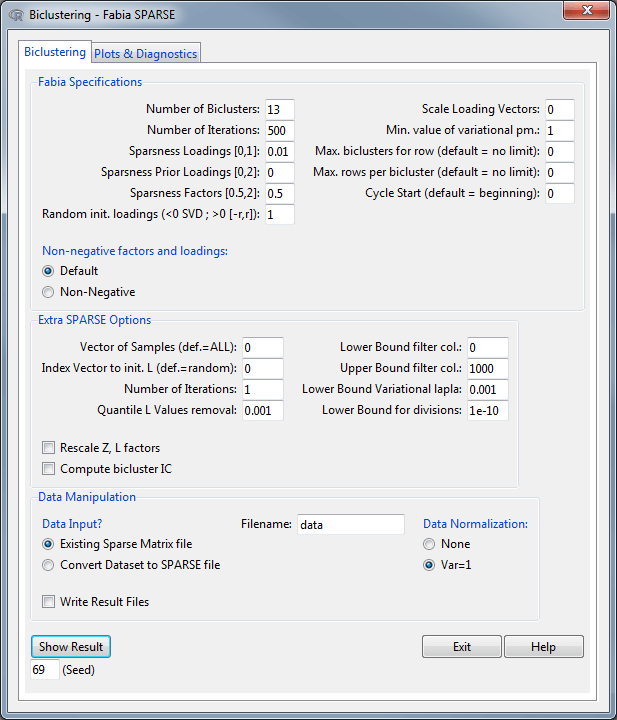
\includegraphics[scale=0.5]{figures/fabia_sparse.png}
\caption{{\it FABIA (SPARSE) Window - Clustering
Tab}\label{fabia_sparse}}
\end{figure}
\noindent Once again, the same specifications as for the {\it Laplace Prior} are
available in this window. However the options for {\it Data Centering} and {\it
Quantile Normalization} are not available anymore.\\
In the second box, {\it Extra SPARSE Options}, more specifications are given,
specific for the SPARSE algorithm. More information about these can be found in
the reference manual and vignette of \verb|fabia| \citep{Hochreiter2014}.
\\ \\
As explained earlier, the algorithm requires the data matrix in a special sparse
format so therefore, the data input for this method works slightly different.
Namely the function requires the data to be located in a plain text file in said
format. There are two options of inputting the data into this algorithm which
will now be explained.\\
The first option assumes that the user already has this text file which contains
the data matrix in sparse format. In this case the {\it Existing Sparse Matrix file}
option should be used and the {\it Filename} entry box should contain the name
of this file (without the extension). Upon pressing the {\it Show Result}
button, the GUI will prompt the user with a directory window in which they have to
select the folder where this file is located.\\
The second option, {\it Convert Dataset to SPARSE file}, will -as the option
states- transform the active dataset in the R commander session to a data matrix
in sparse format. With this option a plain text file will be generated,
containing the data matrix in sparse format with the name inputted in the {\it
Filename} entry box. Now upon pressing the {\it Show Result} button, the user
chooses the folder where this file will be saved. Note that the code behind this
transformation was based on example R-code, available in the \verb|fabia|
vignette \citep{Hochreiter2014a}.\\
Finally, the user can also check the {\it Write Result Files} which will enable
the results being saved in the chosen folder location in the form of plain text
files.
\subsubsection{Fabia: Plots \& Diagnostics}
Similar to the {\it `Plots \& Diagnostics'} of \verb|biclust|, also for
\verb|fabia| the second tab is the same for all of the methods implemented from
this package. The idea is to proceed to this tab after executing the
biclustering method in the first one so that the biclustering result object is
available for the plotting functions. The structure of this {\it Plots \&
Diagnostics window} is given in Figure \ref{fabia_plotdiagtab} which, in this
example, is part of the Laplace Prior dialog.
\begin{figure}[H]
\centering
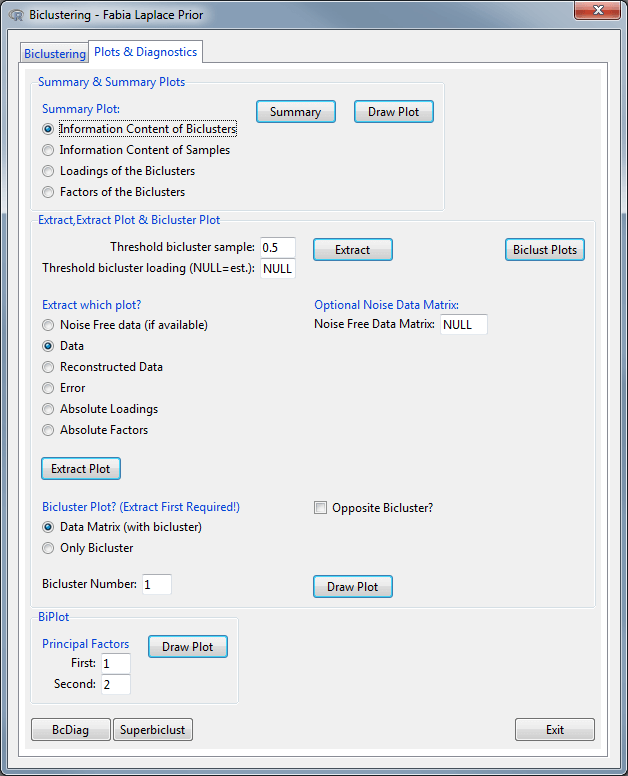
\includegraphics[scale=0.5]{figures/fabia_plotdiagtab.png}
\caption{{\it Fabia Window - Plots \& Diagnostics}\label{fabia_plotdiagtab}}
\end{figure}
\noindent {\bf Summary \& Summary Plots}\\
\noindent By clicking the {\it Summary} button, the user will receive some
general information about the fabia result. Information such as the number of
rows and columns in the data matrix, the number of biclusters, the information
content of the biclusters \& samples and finally some summary statistics of the
column clusters/factors and row clusters/loadings, will be printed in the output
window.\\
Further in this first box, the user can also plot several graphs containing the
information which was outputted by the {\it Summary} button. The first two are
histograms containing the {\it Information Content of Biclusters} and {\it
Information Content of Samples}. The other two options are boxplots of the {\it
Loadings of the Biclusters} and the {\it Factors of the Biclusters}. Examples of
these four types of graphs can be found in the Appendix in figures
\ref{fabiaplot_example1} and \ref{fabiaplot_example2}.\\
More information about the calculation of the information content can be found
in the \verb|fabia| vignette (Hochreiter, 2014). Basically it is a way to rank
the discovered biclusters analogously to principal components which are ranked
according to the data variance they explain. In this case the biclusters are
ranked according to the information they contain about the data.
\\ \\
\noindent {\bf Extract, Extract Plot \& Bicluster Plot}\\
\noindent First of all, in the top of this box, the user is able to extract the
bicluster results from the fabia results object so it can be used for other
applications. This is achieved by using the {\it Extract} button. Before doing
this, 2 thresholds should be set, namely the {\it `Threshold bicluster sample'}
which is a threshold determining when a sample belongs to a bicluster and the {\it `Threshold bicluster loading'} which is, unsurprisingly,
the threshold determining when a loading (=row) belongs to a bicluster. Note
that by default this last one is estimated. The result of this extraction is a
list object which contains the following items: the extracted biclusters and
their indices, the extracted opposite biclusters and their indices, the scaled
and centered data matrix and lastly the number of biclusters. (Opposite means
that the negative pattern is present.)\\
To the right of this button is the {\it Biclust Plots} button which will extract
the biclusters based on the earlier mentioned thresholds and then open up a new
window. This new window contains all the plots and diagnostics from the
\verb|biclust| package.
\\ \\
The next option in this box is the ability to extract more useful plots from
the fabia result. Note that again that the threshold for samples
and loadings apply to these graphs as well. The user is able to pick out of a
multiple of plots, namely the {\it Data}, {\it Reconstructed Data}, {\it Error},
{\it Absolute Factors}, {\it Absolute Factors} and (if available) the {\it Noise
Free data}. For the latter the object name of the noise free matrix should be
entered in the {\it Noise Free Data Matrix} entry box. Interesting to know is
that to achieve sorting, k-means is performed so that the vectors belonging to
the same cluster can be put together. However, in general this sorting is not
able to visualize all biclusters as blocks, namely if they overlap. Several examples of
these plots are given in Figure \ref{fabiaplot_example3} in the Appendix.\\ \\
The final plot is this particular box is the {\it Bicluster Plot} which is
basically the same as the heatmap available in \verb|biclust|. The user is able
to choose a specific bicluster in the {\it Bicluster Number} entry box and then
draw only the bicluster ({\it Only Bicluster}) or the entire data matrix with
the bicluster in the top-left ({\it Data Matrix (with bicluster)}). Further the
user can also decide to plot the opposite bicluster with the {\it Opposite
Bicluster} checkbox. Note that the bicluster plot will {\it only} work if the
extraction in the first part of this box is executed as it requires this output to draw the
biclusters. An example of both graphs can be found in figure
\ref{fabiaplot_example4} in the Appendix.
\\ \\
\noindent {\bf BiPlot}\\
\noindent The final implemented plot in the last box is the {\it BiPlot} for
the matrix factorization result. The user will have to specify the {\it
Principal Factors} that are plotted along the horizontal ({\it First}) and
vertical ({\it Second}) axis. On this biplot, the row-items/genes are
represented as circles with their areas proportional to the row weighting. The
most informative genes are those that are the most distant from the center of
the plot. Note that the column-items are represented by squares. Also for this
last plot type, an example is available in the Appendix in Figure
\ref{fabiaplot_example5}.



\subsection{\texttt{isa2}-package}
The ISA biclustering or {\it Iterative Signature Algorithm} \citep{Bergman2003}
is a semi-supervised method, designed to decompose a large set of data into {\it
modules}. These modules or biclusters consist of subsets of genes (rows) that
exhibit a coherent expression profile only over a subset of
samples/conditions/experiments (columns). ISA does allow for overlapping modules
(rows and columns belonging to multiple modules) and it is developed to find
biclusters that have correlated rows and columns which are identified through an
iterative procedure. A standard ISA procedure starts with normalizing the data
first and then generates random input seeds which correspond to some set of
genes or samples. This is refined at each iteration by adding and/or removing
genes and/or samples until the process converges to a stable set, the {\it
transcription module}. Following now will be the explanation of the {\it ISA
window} in Figure \ref{isa_clusttab} with some more basic information about the
important parameters of the algorithm. More detailed information can however be
found in \citet{Bergman2003} and the \verb|isa2| documentation.
\begin{figure}[H]
\centering
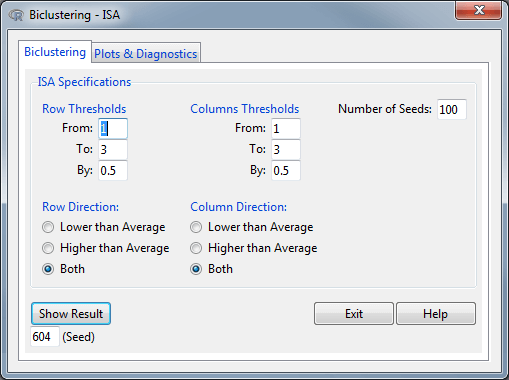
\includegraphics[scale=0.5]{figures/isa_clusttab.png}
\caption{{\it ISA Window - Clustering Tab}\label{isa_clusttab}}
\end{figure}
\noindent The two main parameters of ISA are the two thresholds (for rows \&
columns). If the row threshold is high, then the modules will have very similar
rows, if the threshold is mild, the modules will be
bigger but with less similar rows (analogous for columns). The user is able to
set a sequence of thresholds for both the rows and the columns (default:
\verb|c(1,1.5,2,2.5,3|) and ISA will run over all combinations of these
sequences. For each threshold combination the similar modules will be merged and
as a last step again similar modules will be merged but now across all threshold
combinations. In this last step, if two modules are similar, then the larger one
(with milder thresholds) is kept.\\
Another interesting parameter the user can set is the direction of rows and
columns. This will determine if you are interested in rows/columns that are
higher or lower than the average or even both.\\
The final input value is the number of seeds which are generated to start the
ISA algorithm with. For now the GUI only allows for random seeding, but advanced
user can use the \verb|isa2| package to set non-random seeds which are based on
knowledge of the data (e.g. gene sets).
\begin{figure}[H]
\centering
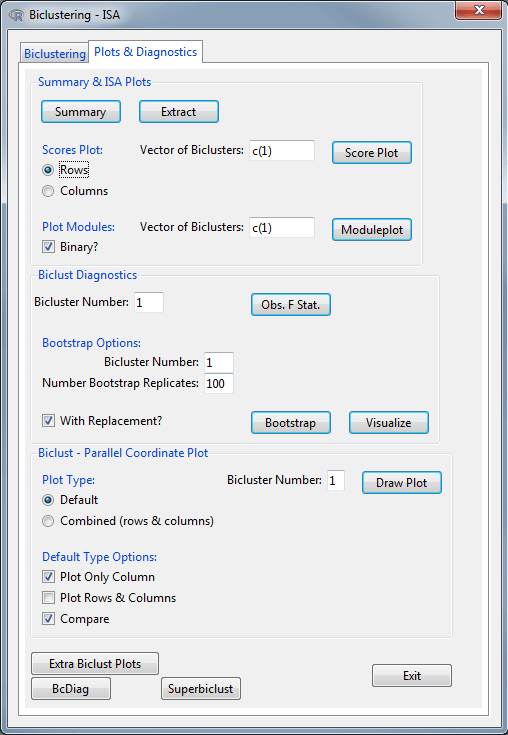
\includegraphics[scale=0.5]{figures/isa_plotdiagtab.png}
\caption{{\it ISA Window - Plots \& Diagnostics Tab}\label{isa_plotdiagtab}}
\end{figure}
\noindent In Figure \ref{isa_plotdiagtab} above, the the second tab for the ISA
method can be found. Apart from the first box {\it `Summary \& ISA Plots'} the plotting and
diagnostic options are the same as for the \verb|biclust| methods therefore they
will not be elaborated on.\\ \\
The {\it Summary} button will give some information about the bicluster result
of \verb|isa2|. It will give the number of found biclusters and report the top
10 biclusters based on the robustness score which is a measure of how well the
rows and columns are correlated. The next button {\it Extract} will transform the
result of \verb|isa| to a list of biclusters and save it in an list-object
called \verb|Extract|. Each entry of this list will have two sublists,
\verb|rows| and \verb|columns| which contain the indices of the subset of rows and
columns.\\
The last two buttons in this box will create graphs based on a user-defined
vector of biclusters (e.g. \verb|c(1,2,3)| = bicluster 1, 2 and 3). The first,
{\it Scores Plot}, will plot either the row or columns scores (depending on the
radio button selection) which is a number between -1 and 1. The further this
number is from zero, the stronger the association of the given {\it row} or
{\it column} to the bicluster. The last, {\it Moduleplot}, will create image
plots for the chosen set of modules as well as the matrix of the original data. The binary
check box will determine whether to binarize the biclusters before plotting or
use the actual ISA scores. An example of these last two graphs can be find in
Figure \ref{isa_example1} in the Appendix.\\
On a final note it should be mentioned that while the {\it extract} and {\it
score plot} functions were not available in the \verb|isa2| package, they were
based on the author's code in the examples of \citet{Csardi2013}.



%note extract and score plot inspired by examples in isa2 tutorial

\subsection{\texttt{iBBiG}-package}
\verb|iBBiG| or {\it Iterative Binary Bi-clustering of Gene Sets} is a
biclustering algorithm proposed by \citet{Gustenleitner2012} which,
similar to {\it Bimax}, will look for submatrices (= modules) of 1's in a spare
binary matrix. But because it works under the assumption of noisy data (non-perfect
binarization), a number of 0's are tolerated within a bicluster. 
Further, it also allows for discovery of overlapping biclusters and the method
is optimized for finding modules in matrices of discretized p-values from gene
set enrichment analysis (GSA). However this does not prevent one to apply it to
any kind of binary matrix. Another attractive feature of iBBiG is that it does
not require prior knowledgde or limit the number or size of clusters.\\
In short, the iBBiG algorithm consists out of three main components: 1) a module
{\it fitness score} 2) a heuristic search algorithm to identify and grow modules
in a high dimensional search space ({\it Genetic Algorithm}) and 3) an iterative
extraction method to mask the signal of modules that have already been
discovered ({\it Iterative Module Extraction}). Further information can be found
in \citet{Gustenleitner2012}.
\\ \\
\noindent The {\it iBBiG window} is shown in Figure \ref{ibbig_clusttab} which
contains the paramaters which iBBiG needs to execute its algorithm.
\begin{figure}[H]
\centering
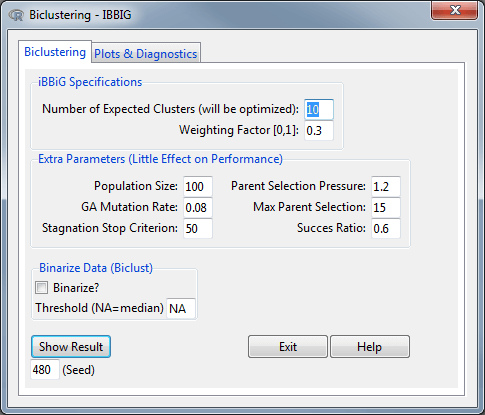
\includegraphics[scale=0.5]{figures/ibbig_clusttab.png}
\caption{{\it iBBiG - Clustering Tab}\label{ibbig_clusttab}}
\end{figure}
\noindent The most important parameter is $\alpha$, the weighting factor, which
is responsible for the balance between module {\it homogeneity} and module
{\it size} when computing the fitness score (number of phenotypes versus number
of genesets, consequently tradeoff between specificity and sensitivity). A small
$\alpha$ wil give more weight to the module size while a large one gives more
weight to the homogeneity. However the authors showed in simulated studies that
a range of 0.3-0.5 is appropriate with an optimal default value of 0.3
\citep{Gustenleitner2012}. However own investigation for a good value for your
particular data or research question is still adviced.\\
The other important parameter is the number of expected biclusters, but because
the algorithm is optimized to find a minimal number, this parameter can be larger
than the expected value. This means it is recommended to choose an upper
boundary for this parameter.
\\ \\
All the other parameters are linked to the genetic algorithm which is a class of
heuristic search algorithms based on evolutionary concepts. It is however
recommended to keep these on default as these input parameters were reported to
have little effect on the results. 
\\ \\
Finally, the active data set in your R Commander session can be binarized if
this is not a binary matrix by default. (This uses the same function available
in \verb|biclust|.) Do note that when plotting graphs (e.g. the biclust plots),
the original data matrix will be used which is the active data set in your
session.
\\ \\
{\it Attention! Results from iBBiG are not reproducible, even when setting a
seed beforehand. The result should be saved if it is to be investigated later.} 
\begin{figure}[H]
\centering
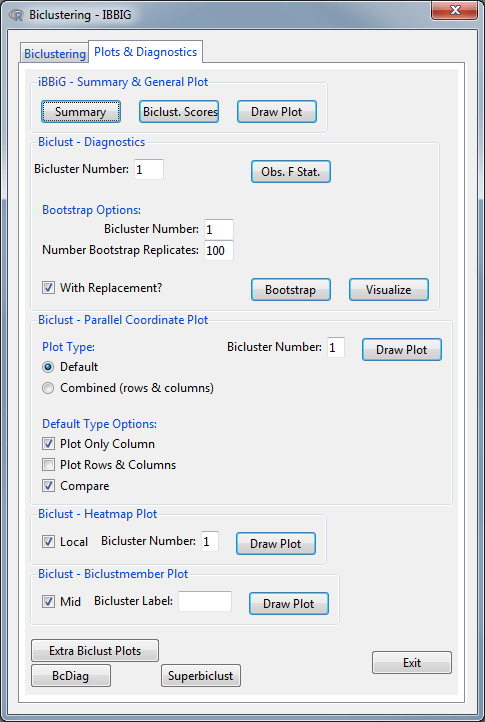
\includegraphics[scale=0.5]{figures/ibbig_plotdiagtab.png}
\caption{{\it iBBiG - Plots \& Diagnostics Tab}\label{ibbig_plotdiagtab}}
\end{figure}
\noindent As can be seen in Figure \ref{ibbig_plotdiagtab}, a lot of the
functionality is the same as for the \verb|biclust| algorithms (Section \ref{sec:biclustplots}) so it therefore
will not be explained again here.\\ \\
On the top, three \verb|iBBiG| specific buttons can be found. The {\it
summary} button will give some basic information about the number of clusters found and
first five biclusters of which the number of rows and columns will be reported.
The next button, {\it Cluster Scores}, will give the module score of the clusters 
and the third one, {\it Draw Plot}, will create a general graph of the
biclustering result. This graph contains a plot of all the modules
colour-labeled in the matrix, as well as some histograms with the module sizes,
module scores and weighted scores. An example of this can be found in the
Appendix in Figure \ref{ibbig_example1}.
\subsection{\texttt{rqubic}-package}
\label{rqubicsection}
The \verb|rqubic| package is the R implementation of QUBIC \citep{Li2009}, a
qualitative biclustering algorithm. The algorithm will first apply quantile
discretization (e.g. 3 levels: unchanged or up- and downregulated) after which a
heuristic algorithm is used to identify the biclusters. In this last step, seeds
will be set which are pairs of gene sharing expression patterns in a number of
samples. By searching for other genes sharing these expression patterns or genes
with an even similar match, the biclusters are identified from this set of
seeds. This is repeated for all the generated seeds and a number of maximal
biclusters (defined as the number of genes times the number of conditions in
that bicluster) are reported.\\
More detailed information about QUBIC can be found in \citet{Li2009}.
\\ \\
\noindent In Figure \ref{rqubic_clusttab}, the {\it rqubic window} can be found
in which all the steps of the algorithm can be set up.

\begin{figure}[H]
\centering
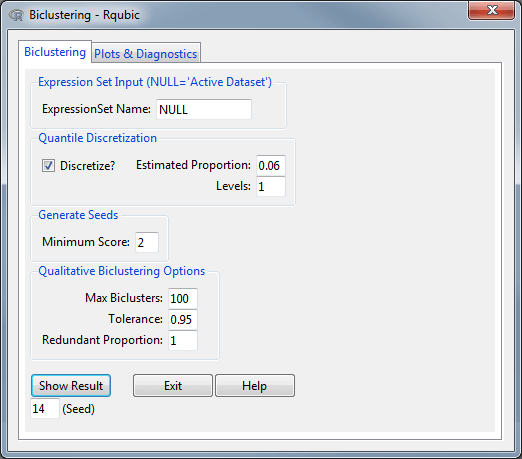
\includegraphics[scale=0.5]{figures/rqubic_clusttab.png}
\caption{{\it Rqubic Window - Clustering Tab}\label{rqubic_clusttab}}
\end{figure}
\noindent Before deciding the parameters, the users has the possibility to use
an ExpressionSet object (\verb|Biobase| package). This was implemented since the
functions of this package primarily accept this kind of object. If no Expression
Set (= eSet) is given here, the active data set will simple be converted to such an
eSet though it will be lack all the additional information an eSet normally
contains (it will only contain the expression matrix). However if the name of an
eSet is given, the expression matrix part of this object will be made the active
data set with the same name as the eSet, appended with `\_expr'. This is done so
it can be used for plotting and diagnostics purposes.\\
In the next part of the dialog, the user gets the option to apply quantile
discretization for which both the number of levels (e.g. level 1 means -1,
0, 1 label) and the estimated proportion of conditions where a gene is up- or
downregulated can be set.\\
The next option is to set the minimum score for the generation of seeds.
A seed is chosen by picking edges with higher scores than this value after composing a complete graph of all genes with coincidence score as weights. This score is the number of samples in which the connected gene pair has the same expression level.\\
Finally, the parameters for the bicluster identifying process can be decided
upon. Parameters such as the maximum number of biclusters ({\it Max Biclusters}), the percentage of
tolerated incoherent samples ({\it Tolerance}) and the proportion of a cluster over which the
cluster is considered as redundant ({\it Redundant Proportion}).

\begin{figure}[H]
\centering
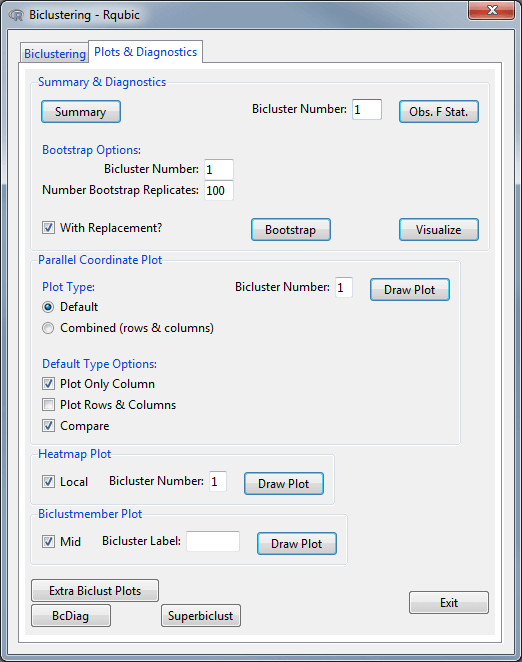
\includegraphics[scale=0.5]{figures/rqubic_plotdiagtab.png}
\caption{{\it Rqubic - Plots \& Diagnostics Tab}\label{rqubic_plotdiagtab}}
\end{figure}
\noindent The second tab (Figure \ref{rqubic_plotdiagtab}) contains the plotting
and diagnostics options which is completely the same as options for the methods
in the \verb|biclust| package.

\subsection{\texttt{BicARE}-package}
The \verb|BicARE| package \citep{Gestraud2014a}, `Biclustering Analysis and
Results Exploration, is centered around the FLOC algorithm \citep{Yang2005} of
which a modified version is implemented.\\
FLOC is a probabilistic {\it move-based} algorithm that can discover a set of
possibly overlapping biclusters simultaneously and is also centered around the idea of
reducing the mean squared residue \citep{Cheng2000}. The authors compared the
results of FLOC on the same yeast data with the algorithms by \citet{Cheng2000}
and they reported that the biclusters returned by FLOC, on average, have a
comparable mean squared residue but a larger size. Further they also reported
that FLOC was able to locate these biclusters much faster than the algorithms
proposed in \citet{Cheng2000}.\\
The FLOC algorithm has two phases. In the first phase, a number of initial
biclusters are constructed by a random process which determines whether a row or
column should be included. Next, the second phase is an iterative process to
improve the quality of the biclusters continuously. In each iteration of the
second phase, each row and column are examined in order to determine the best
action (including/deleting rows/columns,...) towards reducing the overall mean squared residue. Note that sometimes
an action even may be blocked temporarily during an iteration due to a violation of
some constraint. The result of each iteration will be used as the initial
biclustering for the next iteration.\\
A much more detailed description about the algorithm itself and the
incorporation of the parameters which you can set in this algorithm can be found
in \citet{Yang2005}. It also provides more ideas about improvements on the basic
FLOC algorithm, the inclusion of inverted rows (for discovering genes with
opposite regulation) and more.
\\ \\
The {\it BicAre window} is now shown in Figure \ref{bicare_clusttab}.
\begin{figure}[H]
\centering
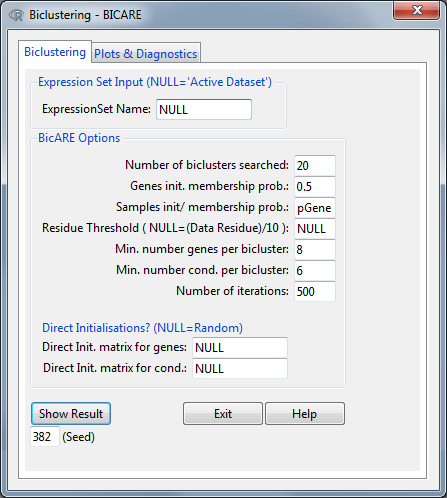
\includegraphics[scale=0.5]{figures/bicare_clusttab.png}
\caption{{\it BicARE Window - Clustering Tab}\label{bicare_clusttab}}
\end{figure}
\noindent Just as for the implementation of the \verb|rqubic| package in the
GUI, the user again gets the possibility to use an `external' Expression Set
instead of only a matrix provided by the Active Dataset (see section \ref{rqubicsection} for
more explanation). For the implementation of this package it is even more
interesting to use an Expression Set object as it will enable the user to apply
gene and sample enrichment in the second tab.\\
In the second box of the biclustering dialog, the user can fill in all the
necessary parameters for the FLOC algorithm which are fairly self-explanatory.
Namely the maximum number of biclusters, the initial membership probability for
genes and samples (in first phase), the residue threshold, the minimum number of
genes and conditions in a bicluster and finally the number of iterations in
phase two.\\ Lastly, instead of random initialisations, the user can also give
the names of matrices which contain information about direct initialisation of
the genes and conditions. These are boolean matrices indicating the membership
of the elements to the biclusters
\begin{figure}[H]
\centering
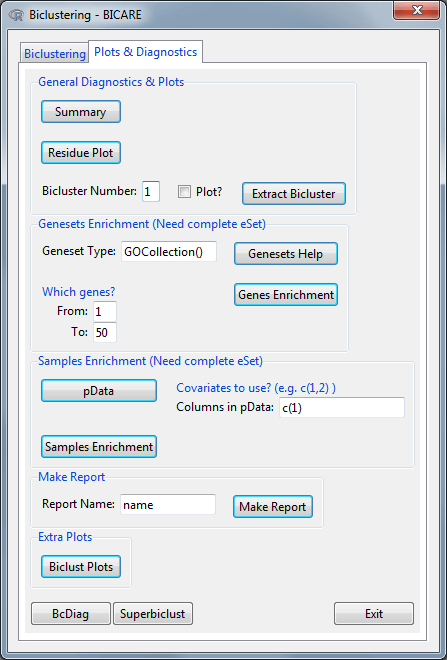
\includegraphics[scale=0.5]{figures/bicare_plotdiagtab.png}
\caption{{\it BicARE - Plots \& Diagnostics Tab}\label{bicare_plotdiagtab}}
\end{figure}
\noindent After applying the algorithm, some BicARE specific plots and
diagnostics are available in the second tab (Figure \ref{bicare_plotdiagtab}). 
\\ \\
\noindent {\bf General Diagnostics \& Plots}\\
The first button in this box, {\it Summary}, will simply print the object as it
is printed when the calculation of the algorithm is done. The next button, {\it
Residue Plot}, will create a plot showing the residues of each of the discovered
biclusters. An example of this graph can be found in the Appendix in Figure
\ref{bicare_example1}. The final button in this box, namely {\it Extract
Bicluster}, will extract the submatrix of the expression matrix corresponding
with the chosen bicluster with the {\it Bicluster Number}. The user can also plot this bicluster by
checking the {\it Plot} option (Figure \ref{bicare_example2} in the Appendix).
\\ \\
\noindent {\bf Genesets Enrichment}\\
In this box, a functional view of the biclusters can be obtained by testing the
over-representation of a priori defined genesets. This over-representation is
evaluated by an hypergeometric test of which the p-values and the adjusted
p-values will be reported. The available genesets are in the GeneSetCollection
format and the {\it Genesets Help} button can be used to query which genesets
are available. These can then be filled in in the {\it Geneset Type} field.
Lastly the user can also decide upon which genes should be used in the
generating of the geneset collection.\\ After the analysis is completed with the
{\it Genes Enrichment} button, the results will be added to the biclustering
result object and the p-values will be printed. It may however be easier to
explore these results with the {\it Make Report} button (see further).\\
Note that this analysis is {\it only} possible when a complete eSet has been
used in the first biclustering tab.
\\ \\
\noindent {\bf Samples Enrichment}\\
This part of the dialog provides the tools to the user to apply a sample
covariates enrichment. First, a button {\it pData} is provided to print the
covariates information of the samples. The user can then choose those columns
from this previous print and put them in vector format. These will be the
covariates which will be used in the actual testing step. Namely for each bicluster, the
enrichment of each level of the covariates will be evaluated with a $\chi^2$
test of adequation.\\
Once again these results will be added to the biclustering results object and a
small part of them will be printed. It is however more convenient to explore
these results afterwards after making the automatic report (see further).\\
Note that again this is only possible if the pData information is available in
the eSet object you have chosen in the first tab.
\\ \\
\noindent {\bf Make Report}\\
Another feature of the \verb|BicARE| package is to build an automatically
generated html report of the biclustering results (and genes/samples enrichment
if this was applied). The user simply needs to provide a name to the report and
then click the {\it Make Report} button. First small window will pop up to
choose the directory in which to put this report after which it will
automatically open in the default web browser (Figure \ref{bicare_example3} in the Appendix).
\\ \\
\noindent {\bf Extra Plots}\\
Finaly, the user can find a button here which will open up a new window which
contains all the \verb|biclust| plots and diagnostics. The correct information
from the \verb|BicARE| will be used and does not require any intervention from
the user itself.

\subsection{\texttt{s4vd}-package}

\subsubsection{SSVD - Biclustering via Sparse Singular Value Decomposition}
Sparse singular value decomposition (SSVD) was first proposed as a biclustering
algorithm by \citet{Lee2010}. It seeks a low-rank checkerboard structured
matrix approximation to data matrices through SVD. \\
For example the following formula shows a rank-$K$ approximation to $\mathbf{X}$
with SVD
$$
\mathbf{X} \approx \mathbf{X}^{(K)} = \sum_{k=1}^K s_k \mathbf{u}_k \mathbf{v}_k^T
$$
in which $\mathbf{u}_k$ and $\mathbf{v}_k$ are the left and right singular
vector.\\
In the SSVD algorithm, biclusters are discovered by forcing the singular
vectors of SVD to be sparse. This is achieved by interpreting the singular
vectors as regression coefficients of a linear model. The algorithm alternately
fits penalized least squares regression models (Adaptive Lasso or Hard
Threshold) to the singular vector pair (left and right) to obtain a sparse matrix decomposition which will then represent the desired checkerboard structure.\\
This procedure minimizes the following formula with respect to the triplet
$(s,\mathbf{u},\mathbf{v})$ in which $P_1 (s \mathbf{u})$ and $P_2 (s
\mathbf{v})$ are the sparsity-inducing penalty terms, and $\lambda_u$ and
$\lambda_v$ the nonnegative penalty parameters
$$
|| \mathbf{X} - s \mathbf{u} \mathbf{v}^T ||^2_F + \lambda_u P_1 (s \mathbf{u}) + \lambda_v P_2 (s \mathbf{v})
$$
The penalty parameters for the optimal degree of sparsity (number of non-zero
coefficients in the singular vector) are determined by minimizing the Bayesian
information criterion (BIC).\\
The SSVD algorithm, to estimate the sparse singular vector pair, is run on the
original data matrix to find the first layer or bicluster. To find the
subsequent biclusters, the algorithm is run on the residual matrix after
subtracting the original matrix with the previous Sparse SVD layer..
\\ \\
While R code for the algorithm was written, it was only later included in the
\texttt{s4vd} R package by \citet{Sill2011a} which this GUI uses.
\\ \\
Figure \ref{ssvd_clusttab} shows the {\it SSVD window}.
\begin{figure}[H]
\centering
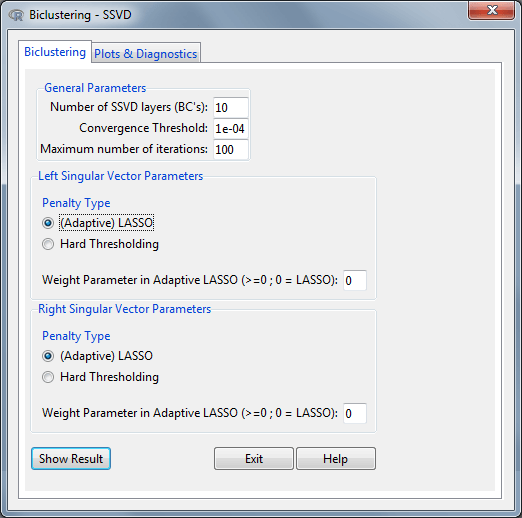
\includegraphics[scale=0.5]{figures/ssvd_clusttab.png}
\caption{{\it SSVD Window - Clustering Tab}\label{ssvd_clusttab}}
\end{figure}
\noindent The biclustering tab with the parameters of the algorithm consists out
of 3 parts. The first part contains some general parameters such as the {\it
number of biclusters} (= SSVD Layers), the {\it number of iterations} and {\it
convergence threshold}.\\
The second and third part contain the penalty type for respectively the left and
right singular vector. Note that for the Adaptive LASSO, the user can specify
the weight. A zero weight would coincide with the normal LASSO.
\\ \\
The second tab is completely similar to the plots \& diagnostics tab of the
\texttt{biclust} packages in Section \ref{sec:biclustplots} so it will not be
discussed here again.

\subsubsection{S4VD - Robust biclustering by ssvd incorporating stability
selection}

The S4VD algorithm by \citet{Sill2011} is an extension of the SSVD algorithm.
They proposed to incorporate stability selection in the original algorithm,
which is a subsampling-based variable selection that allows to control Type I error rates.
The goal was to improve both the selection
of penalization parameters and the control of the degree of sparsity.
Furthermore, the error control also serves as a stopping criterion for the S4VD algorithm and
determines the number of reasonable layers or biclusters.\\
In brief, in each iteration of the alternate estimation and updating of the
singular vector pair, for each possible penalty parameter (separately
of the left and right singular vector) subsamples are drawn and the
relative selection probability of respectively the rows and columns is
estimated. By doing this a stable set of non-zero rows and columns is created
which is then used in the last step to determine the final left and right sparse
singular vectors.\\
Just like for SSVD, this algorithm is applied to find the first layer or
bicluster. To find the next one, the same steps are applied to the residual
matrix after subtracting the rank-one approximation derived by applying a
regular SVD to the submatrix defined by the stable set of left and right
singular vectors.
\\ \\
Presented in Figure \ref{s4vd_clusttab} is the {\it window for S4VD}.
%extension
\begin{figure}[H]
\centering
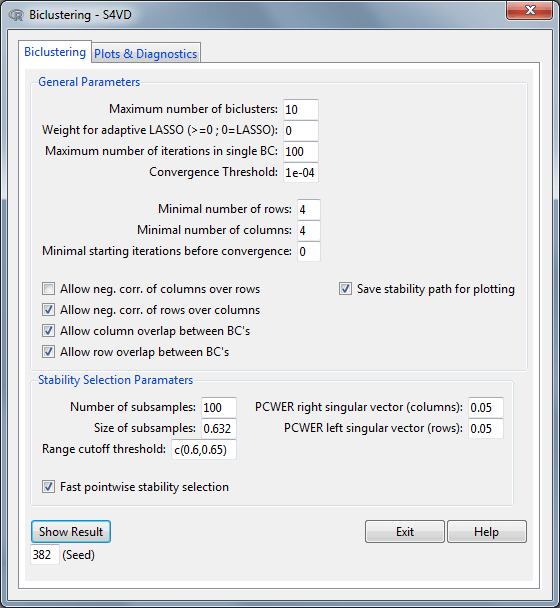
\includegraphics[scale=0.5]{figures/s4vd_clusttab.png}
\caption{{\it S4VD Window - Clustering Tab}\label{s4vd_clusttab}}
\end{figure}
\noindent This time the window is built out of 2 parts. In the first part, which
contains the general parameters, there are some similar parameters as for the
the SSVD algorithm (e.g. {\it Number of biclusters}, {\it Max Iterations}, {\it
Weight Parameter}, {\it Convergence threshold},...). There are also additional
parameters such as the option to save the stability path in order to plot it
later on. However for extreme high dimensional data set, this option might need
to be disabled as the resulting object may exceed the available memory.\\
The second and last part is dedicated to the Stability Selection segment of the
algorithm which contains parameters such as the error rates (= {\it PCWER}).
Since the subsampling steps of the stability selection makes the S4VD algorithm
computationally very demanding, the option is given to use the pointwise error
control to reduce the computation time.

\begin{figure}[H]
\centering
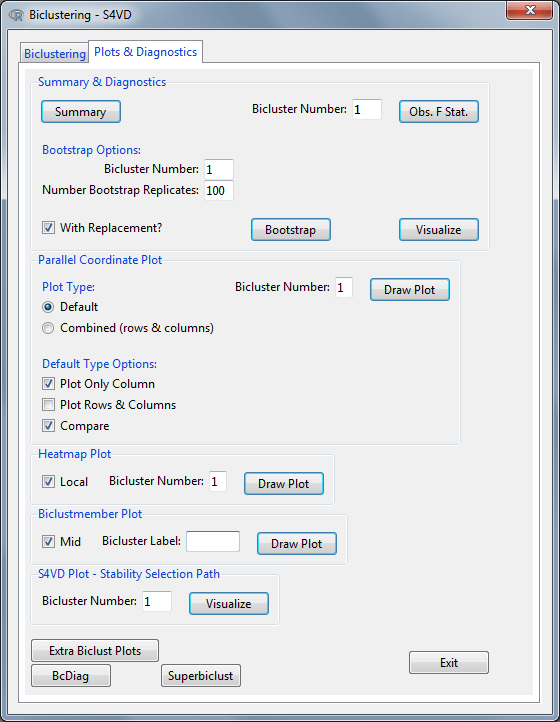
\includegraphics[scale=0.5]{figures/s4vd_plotdiagtab.png}
\caption{{\it S4VD Window - Plots \& Diagnostics Tab}\label{s4vd_plotdiagtab}}
\end{figure}
\noindent Finally, Figure \ref{s4vd_plotdiagtab} shows the {\it Plots \&
Diagnostics window for S4VD}. It is nearly completely the same as the window in
Section \ref{sec:biclustplots} for the \texttt{biclust} package apart from one
addition at the bottom. Here it is possible to plot the stability path for the
rows and columns in a specified bicluster regarding the last iteration. The
path in the plot is basically the selection probabilities for the rows and
columns for the possible penalty parameters. However note that if the pointwise
error control was used, only the final selection probabilities (for the final
penalty parameter) for the rows and columns will be plotted.


\subsection{Diagnostic Packages}
\subsubsection{\texttt{BcDiag}-package}
The first implemented diagnostics package is \verb|BcDiag| which is compatible
with \verb|biclust|, \verb|fabia| and \verb|isa2|. Since the output of \verb|iBBiG|
is an extension of \verb|biclust|, the diagnostics will also work on this
package.\\
\verb|BcDiag|'s task is the visualisation of bicluster data which can be
categorized in three sections:
\begin{enumerate}
  \item Profiling and Summarising the biclustered versus the clustered data
  simultaneously.
  \item Profiling and Summarising the biclustered data only.
  \item Exploring the biclustered data using {\it anova} and {\it median polish}
  techniques.
\end{enumerate}
\noindent A general overview will follow, but more detailed descriptions can be
found in \citet{Aregay2014}.
\\ \\
\noindent In Figure \ref{bcdiag_summary}, the {\it BcDiag Window}
with the accompanying {\it output summary} window are shown. Note that in this example the diagnostics
window was called from a {\it Plaid Window} as can be read in the window title.
\begin{figure}[H]
\centering
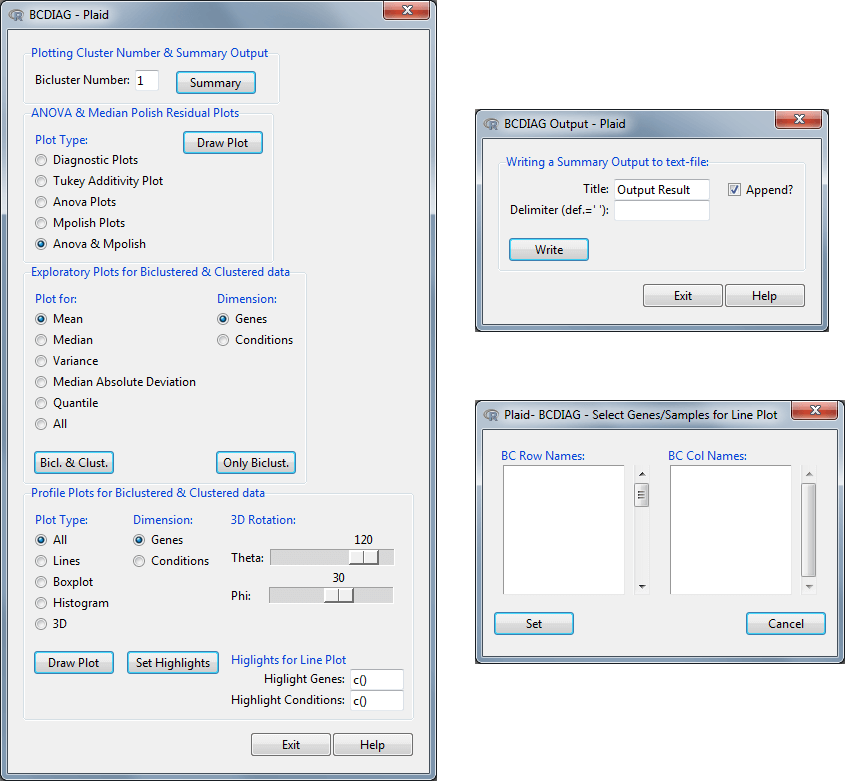
\includegraphics[scale=0.5]{figures/bcdiag_summary.png}
\caption{{\it BcDiag Window with Summary Output Window}\label{bcdiag_summary}}
\end{figure}
\noindent {\bf Summary Output}\\
Using the {\it Summary} button will open up a small new window which can be seen
at the right in Figure \ref{bcdiag_summary}. With the use of this window a
summary output in text format can be created. The user needs to provide a {\it
title} and can also decide on which {\it delimiter} to use (default=space). 
Pressing the {\it write} button will then open up a save window in which the
user can decide on the location and name of the text file which will be created
afterwards.
The original function was developed in the \verb|biclust| package and will
create a text file with the total number of biclustered, the dimension and the name of
biclustered rows and columns.
\\ \\
\noindent {\bf Bicluster Number}\\
At the top of the {\it BcDiag Window} the user can set the number of the
bicluster for which the graphs should be created. This value is used for all the
plots down in the window apart from of course the summary button which extracts
all biclusters.
\\ \\
\noindent {\bf ANOVA \& Median Polish Residual Plots}\\
Here residual plots or residual box plots for a bicluster can be created. These
can be diagnostic plots (fitted vs residual, QQ,\dots), {\it Tukey additivity
plots}, {\it anova} and {\it mpolish} plots. An example of some of these graphs
can be found in the Appendix in Figure \ref{bcdiag_example1}.
\\ \\
\noindent {\bf Profile Plots}\\
With this graph, profile plots for biclustered data can be created. These
profile plots can either be in {\it lines}, {\it boxplot}, {\it histogram} or
even {\it 3D} format.
For this last type the rotation can be controlled by the {\it theta} and {\it
phi} parameter, respectively the {\it z} and {\it y} azis. Further, the user can
decide to either to make these profile plots on the {\it genes} (=rows) or {\it
conditions} (=columns) dimension. If for example you would choose the conditions
dimension and lines as type, you would get the same result as the {\it parallel
coordinates plot} (combined type) from the \verb|biclust| plots. In this
scenario each line is a gene in the bicluster and it gets a red colour labeling
if the column also is a part of the bicluster. The other way around, namely
choosing the genes dimension, would mean that each line is one condition which
is red when the gene on the x-axis is part of the bicluster. Some examples of these
are shown in Figure \ref{bcdiag_example2} in the Appendix.\\
Further, there is also an option to highlight gene or condition profiles for the
line plot type. Either give a vector with indicies or character names in the
{\it Highlight Genes/Conditions} boxes, or use the {\it Set Highlights} button
to open up a new window as shown in Figure \ref{bcdiag_summary}. This dialog
will show a list of the gene and conditions names of the chosen
bicluster. From this list the to-be-highlighted members can be selected and
after pressing {\it Set}, the highlight vectors will be filled out corresponding
to this selection.
\\
\\
\noindent {\bf Exploratory Plots}\\
These plots are summary plots for the {\it mean}, {\it median}, {\it variance},
{\it MAD} and {\it quantiles} of the data. Just like for the profile plots, the
dimension can be chosen here as well. Lastly the user can decide to show both
the in-bicluster and out-bicluster information with the left button {\it Bicl. \& Clust.} (as is
always the case for the profile plots) or only the in-bicluster information with
the {\it Only Biclust.} button. This is basically just the first part of the graph
with both the in- and out-bicluster information as can been seen in figure
\ref{bcdiag_example3} in the Appendix.
\\ \\
\noindent {\bf Note on FABIA Results}\\
For results from \verb|FABIA| it is possible to set sample and loading
thresholds to determine the biclusters (Figure \ref{bcdiag_fabia}).
\begin{figure}[H]
\centering
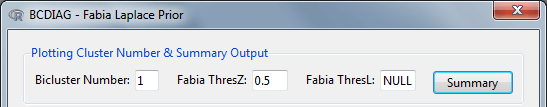
\includegraphics[scale=0.5]{figures/bcdiag_fabia.png}
\caption{{\it BcDiag - Fabia Thresholds}\label{bcdiag_fabia}}
\end{figure}

\subsubsection{\texttt{superbiclust}-package}
A central issue of biclustering is its stability which can highly influence the
ability to interpret the results of a biclustering analysis. The stability can
be affected by initialisation, parameter settings and perturbations such as
random noise. \citet{Shi2010} introduced a novel procedure for obtaining
robust biclusters from a set of initial values which is exactly what
\verb|superbiclust| will accomplish. It will construct a hierarchy of
biclusters based on for example the Jaccard index from which the robust
biclusters based on this `superbiclust' concept can be extracted.\\
\noindent Starting now, the functionality of the {\it superbiclust window} will
be explained, following the default structure of a superbiclust analysis.
However, for more information about the architecture of \verb|superbiclust|, see
\citet{Khamiakova2013} and see \citet{Shi2010} for more details
about the `superbiclust' concept itself.
\begin{figure}[H]
\centering
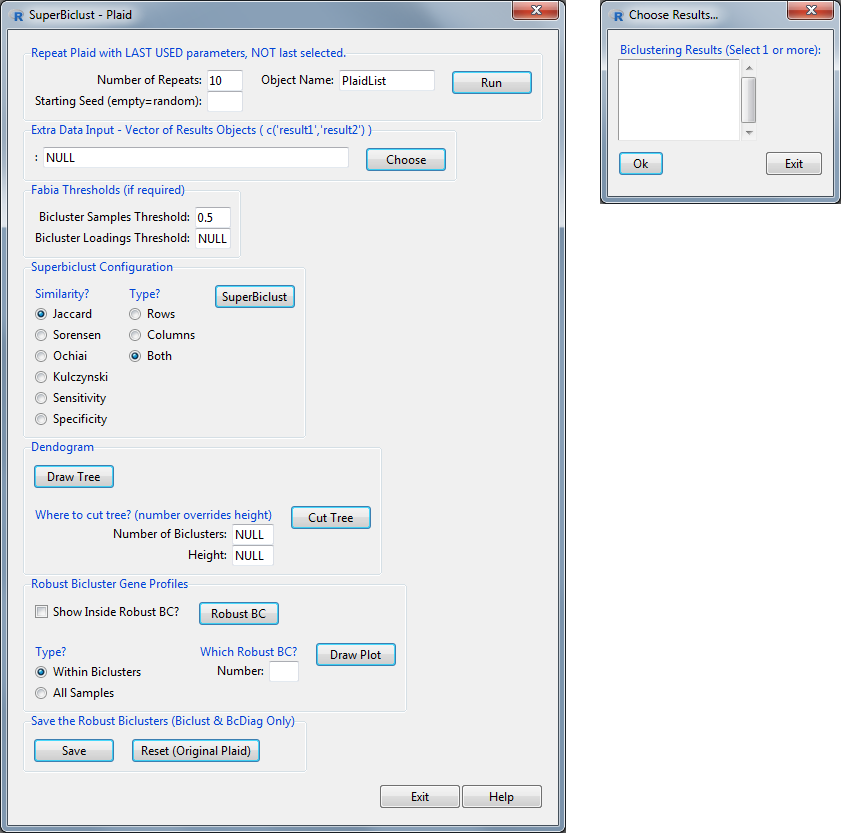
\includegraphics[scale=0.5]{figures/superbiclust.png}
\caption{{\it Superbiclust Window}\label{superbiclust}}
\end{figure}
\noindent {\bf Repeat 'Method' with LAST USED parameters, NOT last selected.}\\
Inside this first box of the Superbiclust window, it is possible to repeat the
selected method multiple times and then easily feed it into the superbiclust
framework in addition to the original result. Pressing the {\it Run} button will
repeat the analysis for the chosen {\it Number of Repeats} and save these
results in a list object with the chosen name of {\it Object Name}. It is also possible to set a starting seed of
this analysis in the {\it Starting Seed} field. Leaving this field empty will
choose a random seed (and print which one).\\
Note that the chosen parameters for these repeats will be the {\it last used}
parameters, not the {\it currently selected}. This is to ensure that the chosen
parameters do not result in an error or nonsensical output.\\
After the analysis is complete, the object will automatically be pasted in the
{\it Extra Data Input} field to introduce it into the superbiclust framework.\\
Finally, note that this list object of biclustering results can also be saved as
an .RData object through {\it 'Help \& Utilities', 'Save/Load'} (See Section
\ref{sec:SaveLoad}). Saving multiple repeated analysis in either R objects or
.RData files will also enable you to compare multiple parameter settings of a
specific method. Simply repeat the analysis with multiple parameter choices,
save these in different list objects, and then input these objects in the {\it
Extra Data Input} field.
\\ \\
\noindent {\bf Extra Data Input}\\
\noindent First of all, at the top of the window in Figure \ref{superbiclust},
there is room to add other biclustering results objects which are loaded in the
R workspace. The format should be as in the given example:
\verb|c('result1','result2')|. The easiest way to do this is to use the {\it
Choose} button. This will open up a small new window in which the user can
select those results of interest. After pressing {\it Ok}, they will be
immediately filled in in the entry field.\\
Note that result objects added in this field are always {\it in addition} to the
result of the original analysis in the first tab.
\\ \\
\noindent {\bf Fabia Thresholds}\\
\noindent In this small box, the user can set the thresholds for biclustering
results from \verb|Fabia|. These thresholds will apply for all the selected
fabia results for the extra data input as well as for fabia result on which the
superbiclust might be originally used. This means that the box will always be
available.
\\ \\
\noindent {\bf Superbiclust Configuration}\\
In this box, the first part of a superbiclust analysis is executed, namely the
computation of the similarity matrix of the biclusters. In this figure, we are
working with the results of the plaid method as can be seen in the title window.
This matrix can be based on several types of similarity and the user can
also decide to base it on the rows, columns or on both (as is suggested for bicluster
results). (Note that for fabia results, the default threshold is used to determine the biclusters.)
\\ \\
\noindent {\bf Dendogram}\\
In the next step, the similarity matrix will be used to construct a hierarchical
tree. This is visualised in a dendogram which can be drawn with the {\it Draw
Tree} button of which an example is given in Figure \ref{superbiclust_example1} 
(Appendix).\\
By cutting this tree now, the {\it robust} or {\it super biclusters} can be
obtained. This user can do this either by setting a {\it number} of desired
{\it biclusters} or by choosing an appropriate {\it height} to cut the tree at
before using the {\it Cut Tree} button.
\\ \\
\noindent {\bf Robust Bicluster Gene Profiles}\\
After cutting the tree, some information can be called with the {\it Robust BC} 
button with or without the {\it Show Inside} checkbox. The result of this can be
found in Figure \ref{superbiclust_example2} in the Appendix. In first part a
matrix is presented with in the first row the index of the robust bicluster and
in the second row the number of original biclusters it contains. Note that only
those robust biclusters created from more than one bicluster will be displayed.
The second part, which will appear if you check the {\it Show Inside} option,
will tell you the indices of the original biclusters in a robust bicluster.\\
In the last part of this box, the user is able to quickly draw a profile plot of
a robust bicluster of choice. Just like in the {\it Bcdiag Window}, either all
the data (in-bicluster + out-bicluster) or only the in-bicluster data can be
drawn. 
\\ \\
\noindent {\bf Save the Robust Biclusters}\\
The last box gives the user the option to {\it save} the robust biclusters. By
doing this, the user can go back to the previous window (plots \& diagnostics
tab) or even to the {\it bcdiag} window (or extra {\it biclust plots}). If the user creates the graphs now,
they will be based on the robust biclusters instead of the original ones.
However, take note that this only applies to the
\verb|biclust|-plots/diagnostics and the plots created by \verb|bcdiag|. 
For example in the case of \verb|isa2|, the user will not be able to create the
correct scores or modules plots as this information is lost after combining
biclusters into a robust one. Another example would be the buttons in the {\it
`summary \& general plot'} box of \verb|iBBiG|. Same goes for \verb|fabia|,
only the plots from \verb|biclust| and \verb|BcDiag| will now work. If you would
like to go back to the original bicluster result, simply click the {\it Reset Button}.


\newpage
\section{A Guideline to New Implementations}\label{sec:guideline}
Thanks to the easy plug-in extensibility of R Commander, adding new dialogs is
very simple. One only needs to make the desired window function and then add
this to the \verb|menus.txt| file situated in the plugin package folder
(\verb|package -> inst -> etc|) as explained in \citet{Fox2007}.\\
If you are familiar with the \verb|Rcmdr| and \verb|tcltk| syntax, you can make
your own customized dialog functions and then send these to the maintainer of
\verb|RcmdrPlugin.BiclustGUI|. \\ \\
However, if you are new to these two packages or simply want an easier and
quicker way to construct your biclustering dialogs, {\it template functions} have been
created to help with this process. In the following sections, an explanation
will be given on {\it two kinds of scripts} in which these functions are called to
create your desired window. 
\begin{description}
  \item[$\bullet$ {\bf New Method Script: }] The {\it first} type of {\it script } will adress the creatiion of a
  dialog to execute biclustering methods.
  \item[$\bullet$ {\bf New Tool Script: }] The {\it second} type of {\it script } adresses the creation of an extra
  tool window. This last one can serve as either an extension of the first (through buttons) or can be a
general diagnostic window compatible with multiple methods. This will be
further discussed in a later section.
\end{description}
\noindent It should also be noted that these templates are specifically tailored
to biclustering methods and that all of the already implemented methods are done
through these scripts.
\\ \\
In the end, what should be given to the maintainer to implement a new method are
the following items:
\begin{enumerate}
  \item The necessary window scripts (manually or through the templates)
  \item A simple description of how the menu should look like in R Commander
  (e.g. Biclust menu opens up into several subitems like plaid, Xmotifs,\dots ).
  \item  A function to transform the results object of the new method to a
  \texttt{biclust} object. This is a S4 class object of which the most important
  slots are \texttt{RowxNumber}, \texttt{NumberxCol} and \texttt{Number} (see
  \texttt{Biclust-class} in the \texttt{biclust} reference manual
  \citep{Kaiser2014}.
  This ensures that the new package will be immediately compatible with the
  \texttt{BcDiag} and \texttt{superbiclust} packages as well as all the
  {\it Extra Utilities} the GUI offers.
  \item {\it Optional:} The correct criteria which should be used in the {\it Search Window}
\end{enumerate}
 



\subsection{Implementing a New Method}

\noindent For starters, each biclustering window is made out of two tabs.
One to execute the method and one to show diagnostics and plots. Both tabs have
some standard buttons which will appear at the bottom as well as some optional
ones as depicted in Figure \ref{stdbuttons}.
\begin{figure}[H]
\centering
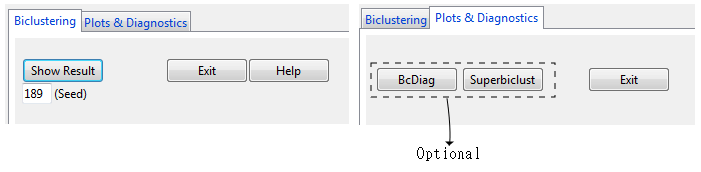
\includegraphics[scale=0.5]{figures/standard_buttons.png}
\caption{{\it Standard Tab Buttons}\label{stdbuttons}}
\end{figure}
\noindent As will become clear later, the clustering tab will
contain the parameters of the biclustering method while the second tab will
contain diagnostics and plots {\it specific} to this method. The concept is that
the optional buttons will lead to new windows of general diagnostic packages,
compatible with multiple biclustering methods.
\\ \\
\noindent Secondly, the idea is to have one biclustering function/method for
each biclustering dialog and tailor it towards this. 
\\ \\
\noindent Lastly, also note that the generation of the R code in the script window, one
of R Commander's advantages, is also done automatically through the use of
the template scripts.


\subsubsection{New Method Script - ClusterTab \& PlotDiagTab}
\label{sec:newmethodscript}
We will now start going through \verb|newmethod_script.R| which can be found in
the Appendix.\\
The script \verb|newmethod script.R|, the first type of the mentioned scripts,
can be used in order to create a new window for a new application.
\\ \\
\noindent {\bf \underline{General Method Information}}\\
\noindent The script begins by opening a function which will be closed again
after the final step of the script. Here, this function is called \verb|newmethod_WINDOW|,
but this can be changed to one's own window name. This function will be called
by R Commander to make the accompanying window appear when accessing
the menus.\\
Next, some objects are initialized (\verb|new.frames|, \verb|grid.config| and
\verb|grid.rows|). These will be used to store information in about your window
you are about to create.


\begin{knitrout}
\definecolor{shadecolor}{rgb}{0.969, 0.969, 0.969}\color{fgcolor}\begin{kframe}
\begin{alltt}
\hlstd{newmethod_WINDOW} \hlkwb{<-} \hlkwa{function}\hlstd{()\{}

        \hlstd{new.frames} \hlkwb{<-} \hlkwd{.initialize.new.frames}\hlstd{()}
        \hlstd{grid.config} \hlkwb{<-} \hlkwd{.initialize.grid.config}\hlstd{()}
        \hlstd{grid.rows} \hlkwb{<-} \hlkwd{.initialize.grid.rows}\hlstd{()}

        \hlcom{#####################################################}
        \hlcom{## GENERAL INFORMATION ABOUT THE NEW METHOD/WINDOW ##}
        \hlcom{#####################################################}

        \hlstd{methodname} \hlkwb{<-} \hlstr{"A new method"}

        \hlstd{methodfunction} \hlkwb{<-} \hlstr{"methodfunction"}
        \hlstd{data.arg} \hlkwb{<-} \hlstr{"d"}
        \hlstd{methodshow} \hlkwb{<-} \hlnum{TRUE}
        \hlstd{methodsave} \hlkwb{<-} \hlnum{TRUE}
        \hlstd{other.arg} \hlkwb{<-} \hlstr{""}
        \hlstd{methodhelp} \hlkwb{<-} \hlstr{""}

        \hlcom{# Transform the data from data.arg}
        \hlstd{data.transf} \hlkwb{<-} \hlstr{"matrix"} \hlcom{# Values: "matrix" (default), "ExprSet"}

        \hlcom{# Extra Data Conversion Boxes}
        \hlstd{data.discr} \hlkwb{<-} \hlnum{FALSE}
        \hlstd{data.bin} \hlkwb{<-} \hlnum{FALSE}

        \hlcom{# Possibility to give a seed ?}
        \hlstd{methodseed} \hlkwb{<-} \hlnum{TRUE}

        \hlcom{## COMPATIBILITY? ##}

        \hlcom{# BcDiag}
        \hlstd{bcdiag.comp} \hlkwb{<-} \hlnum{FALSE}

        \hlcom{# SuperBiclust}
        \hlstd{superbiclust.comp} \hlkwb{<-} \hlnum{FALSE}


\hlstd{\}} \hlcom{# Note: The curly bracket is placed here for syntax reasons. }
  \hlcom{#       It should be placed after the call of cluster_template.}
\end{alltt}
\end{kframe}
\end{knitrout}
\noindent The scripts starts by filling in some information about your
biclustering method. A clarifying example follows later, filling in this
information for the Plaid method.
\begin{description}
  \item[$\bullet$ \texttt{methodname}:] The title of the window which will be
  shown on top. It may contain no special characters besides `-'. It is
  important to know that the result of your biclustering function will be saved in
  a global variable, named \verb|methodname| without the spaces and `-' symbols.
  Therefore, do not make this string too elaborate.
  \item[$\bullet$ \texttt{methodfunction}:] A string which contains the name of
  your biclustering method's function. By this the actual R function,
  corresponding with the method, is meant. Note that the R command (which is printed in the script
window of R Commander) to execute the biclustering algorithm actually
starts with this string. New arguments are appended to this string until the
R command is fully constructed.
  \item[$\bullet$ \texttt{data.arg}:] The name of the argument which needs the
  data.
  \item[$\bullet$ \texttt{methodshow}:] Logical value which decides if the the
  object in which the clustering result is saved, should be printed. See figure
  \ref{showmethod}.
  \item[$\bullet$ \texttt{methodsave}:] {\bf -Warning: Experienced Users-} A logical value which decides if the
  the result of the {\it methodfunction} should be saved or not. Putting this
  argument to \verb|FALSE| is only advised when knowing the use of
  \verb|doItAndPrint()| and \verb|justDoIt()|. This option can be useful in the
  scenario where the biclustering method actually consists out of multiple steps
  of functions. You can then create a general `GUI' function which does not
  return an object (therefore the saving is not required), but will use
  \verb|doItAndPrint()| to execute the different functions. However do make sure
  that eventually the result is saved in an object as described in the
  explanation of \verb|methodname|. This is to ensure the plotting functions can
  use the correct result. (The \verb|rqubic| implementation is an example of this) 
  (Note that putting \verb|methodsave| to \verb|FALSE| will also put methodshow
  to \verb|FALSE|)
  \item[$\bullet$ \texttt{other.arg}:] A string containing extra arguments that cannot be changed
by the user. For example, in the plaid window, it is used as follows. Since the
biclust package uses only one function to execute all the different methods,
namely \verb|biclust()|, for the plaid method the string
\verb|",method='BCPlaid'"| is added. Note the use of the comma in the beginning of the string! This is
because this string is not restricted to only one argument, it could contain
several of them. They simply need to be added in this string as they would
be added inside the function itself.  
  \item[$\bullet$ \texttt{methodhelp}:] The name of the helppage the help button
  should be directed to. (\verb|help(methodhelp)|)
  \item[$\bullet$ \texttt{data.transf}:] Value which will determine if the data
  for \verb|data.arg| should be transformed or not. Possible values are
  \verb|""| for no conversion, \verb|"matrix"|(default) for \verb|as.matrix| and
  \verb|"ExprSet"| to convert it to an ExpressionSet obect
  (\texttt{Biobase}-package).
    \item[$\bullet$ \texttt{data.discr}:] Logical value determining if a frame
  should be added above the {\it Show Results} button with the option to
  discretize the data. The \verb|discretize| function from the \verb|biclust|
  package is used to achieve this. See Figure \ref{discr.bin}.
  
  \item[$\bullet$ \texttt{data.bin}:] Logical value determining if a frame
  should be added above the {\it Show Results} button with the option to
  binarize the data. The \verb|binarize| function from the \verb|biclust|
  package is used to achieve this. See Figure \ref{discr.bin}.
  
  \item[$\bullet$ \texttt{methodseed}:] Logical value determining if there
  should be a seed box below the {\it Show Results} button. This will make sure
  a \verb|set.seed()| is executed before the biclustering function. Further,
  methods with \texttt{methodseed==TRUE} will also have the feature enabled in
  the superbiclust window to repeat the analysis multiple times.
  
  \item[$\bullet$ \texttt{bcdiag.comp} \& \texttt{superbiclust.comp} :] Logical
  value determining compatibility with the \verb|BcDiag| and \verb|superbiclust|
  package respectively. Please note that this only enables the appearance of the
  buttons in the second tab. For a button to function properly, some minor
  coding needs to be carried out by the maintainer.\\
  (Note that if a transformation function to a \verb|biclust| object is given,
  namely the format in which the results of methods in the \verb|biclust|
  package are, this almost requires no work on the maintainer's side)
  
\end{description}

\begin{figure}[H]
\centering
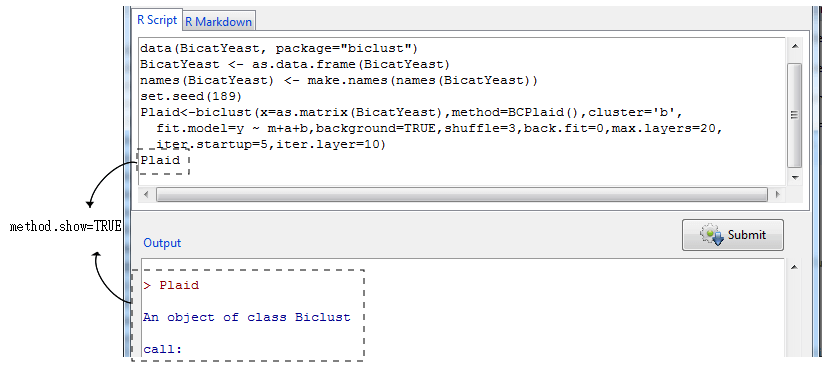
\includegraphics[scale=0.5]{figures/showmethod.png}
\caption{{\it Example of Plaid Biclustering - With} \texttt{method.show=TRUE}
\label{showmethod}}
\end{figure}
\begin{figure}[H]
\centering
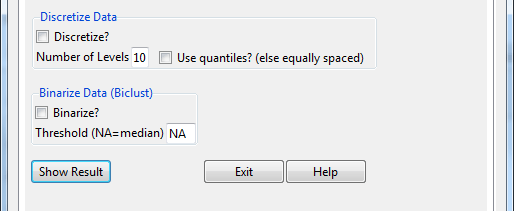
\includegraphics[scale=0.5]{figures/discrbin.png}
\caption{{\it Example of discretize and binarize frames.}
\label{discr.bin}}
\end{figure}

\noindent {\bf \underline{Cluster Tab}}\\
After providing the information about the new biclustering method, the window
for it can be created. Note that whatf ollows is simply appended to the
previous part of the script, but still inside the \verb|newmethod_WINDOW|
function which was opened in the very beginning.\\
Both the clustering tab and the plotting \& diagnostics tab are created
in three easy steps as shown in Figure \ref{threesteps}:
\begin{enumerate}
\item Making the frames
\item Configuring the frames into a grid
\item Combining rows into a box
\end{enumerate}

\begin{figure}[H]
\centering
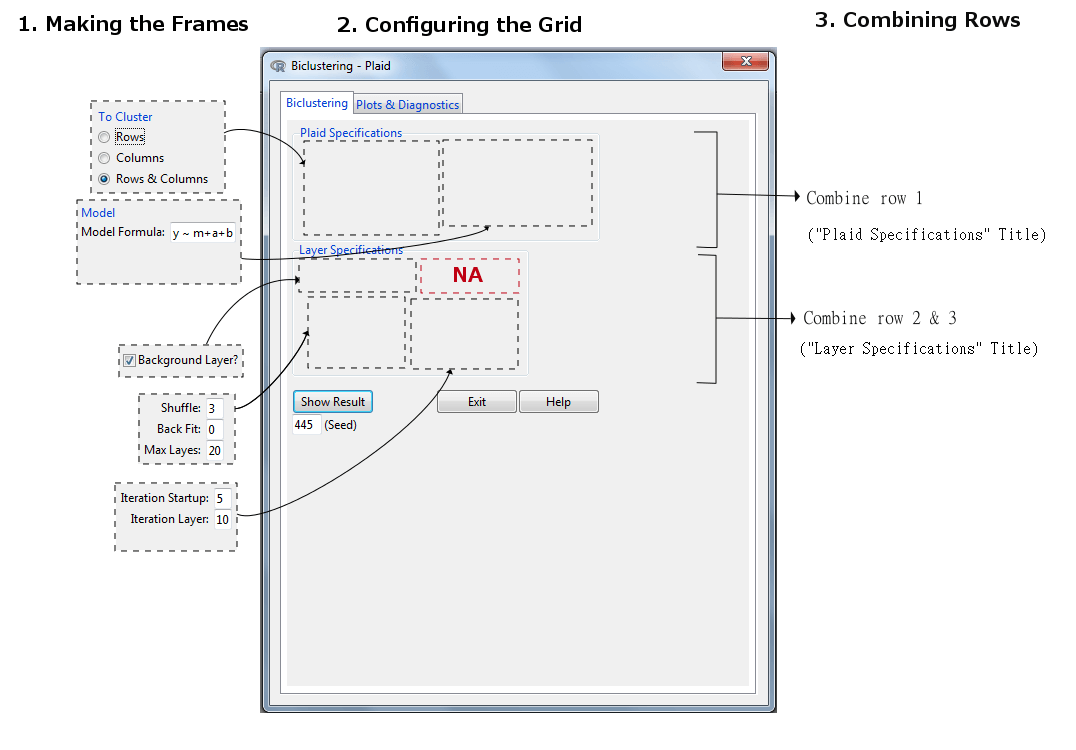
\includegraphics[scale=0.44]{figures/plaid_structure.png}
\caption{{\it Making windows in 3 steps}
\label{threesteps}}
\end{figure}
\begin{knitrout}
\definecolor{shadecolor}{rgb}{0.969, 0.969, 0.969}\color{fgcolor}\begin{kframe}
\begin{alltt}
\hlcom{########################}
\hlcom{#### CLUSTERING TAB ####}
\hlcom{########################}

\hlstd{input} \hlkwb{<-} \hlstr{"clusterTab"}

\hlcom{### 1. ADDING THE FRAMES ###}

\hlcom{# Add frames here}

\hlcom{### 2. CONFIGURING THE GRID ###}

\hlstd{grid.config} \hlkwb{<-} \hlkwd{.grid.matrix}\hlstd{(}\hlkwc{input}\hlstd{=input,}\hlkwd{c}\hlstd{(}\hlstr{"frame1"}\hlstd{,}\hlstr{"frame2"}\hlstd{,}\hlstr{"frame3"}\hlstd{,}\hlnum{NA}\hlstd{,}\hlstr{"frame4"}\hlstd{,}\hlnum{NA}\hlstd{),}
                    \hlkwc{nrow}\hlstd{=}\hlnum{3}\hlstd{,}\hlkwc{ncol}\hlstd{=}\hlnum{2}\hlstd{,}\hlkwc{byrow}\hlstd{=}\hlnum{TRUE}\hlstd{,}\hlkwc{grid.config}\hlstd{=grid.config)}


\hlcom{### 3. COMBING THE ROWS ###}

\hlstd{grid.rows} \hlkwb{<-} \hlkwd{.combine.rows}\hlstd{(}\hlkwc{input}\hlstd{=input,}\hlkwc{rows}\hlstd{=}\hlkwd{c}\hlstd{(}\hlnum{1}\hlstd{),}\hlkwc{title}\hlstd{=}\hlstr{"A nice box: "}\hlstd{,}
                    \hlkwc{border}\hlstd{=}\hlnum{TRUE}\hlstd{,}\hlkwc{grid.rows}\hlstd{=grid.rows,}\hlkwc{grid.config}\hlstd{=grid.config)}
\hlstd{grid.rows} \hlkwb{<-} \hlkwd{.combine.rows}\hlstd{(}\hlkwc{input}\hlstd{=input,}\hlkwc{rows}\hlstd{=}\hlkwd{c}\hlstd{(}\hlnum{2}\hlstd{,}\hlnum{3}\hlstd{),}\hlkwc{title}\hlstd{=}\hlstr{"A nice box: "}\hlstd{,}
                    \hlkwc{border}\hlstd{=}\hlnum{TRUE}\hlstd{,}\hlkwc{grid.rows}\hlstd{=grid.rows,}\hlkwc{grid.config}\hlstd{=grid.config)}
\end{alltt}
\end{kframe}
\end{knitrout}
\noindent Looking at the script, you can see it starts with putting the
\verb|input| to {\it clusterTab}. This will make sure everything you are
creating and saving now will be done for the first tab, namely the clustering
tab.
\\
\\
{\it Step 1:}\\
As already explained earlier, the first step will be to create the frames in
which you want to put your function arguments. A variety of frames can be
created, but these will be explained in more detail in the following section. To
give a quick summary, here is the list of the types of frames which can be
generated in the clustering tab.
\begin{itemize}
  \item Check Boxes
  \item Radio Buttons
  \item Entry Fields
  \item Sliders
  \item Spinboxes
  \item Manual Buttons (only for plot \& diagnotics tab)
\end{itemize}
\noindent In future updates, there is still the possibility to add even more
types if required.
\\ \\
{\it Step 2:}\\
During the creation of the frames in the previous step, you will have given each
of them a unique name. Using these framenames, the next step will be to simply
order them into a matrix grid, filling in the empty spots with \verb|NA|'s.
This is achieved with the \verb|.grid.matrix| function. The function accepts
the exact same arguments as the \verb|matrix| function apart from two new ones,
namely \verb|input| and \verb|grid.config|. The first is to make sure the
template function knows we are adding frames in the first tab, while second one
is there to ensure that the new information is added to the old
\verb|grid.config| object and that old information is not lost.\\
Further, it is important to know that the inserted frames will {\it always} be
pulled towards the north-west as much as possible. Therefore in a 1-row
matrix, something like \verb|c(NA,"frame1")| or \verb|c("frame1",NA)| would give
exactly the same result.
\\ \\
{\it Step 3:}\\
The final step will enable you to put one or multiple rows in a seperate box
which can serve two different purposes. The first is 	to add some visual
distinction between rows with the help of a title with or without a border around the row(s).\\
The second purpose is connected to the way frames are added in this {\it grid}.
Sometimes if frames have a large difference in size, other frames might seem to
be jumping to the right, trying to fit in one general grid. In general if you
see this happening, putting this row(s) in a box will solve this problem and the
frames will again be pulled towards the left (see Figure \ref{combinerows_grid}
for an example). This works because now the grid exists 'locally' in this row
box.\\
Creating these boxes by combining rows is very easy, simply use the
\verb|.combine.rows| function which will save the necessary information in the
\verb|grid.rows| object. The function only has three arguments that should be
changed: (1) \verb|rows| - a vector containing the rows you wish to combine,
 (2) \verb|title| - give the box a title (\verb|""| means no title) and
(3) \verb|border| - determines if there should be a border.\\
Note that in contrast to the grid configuration, you can call this function
multiple times until the desired result is obtained.

\begin{figure}[H]
\centering
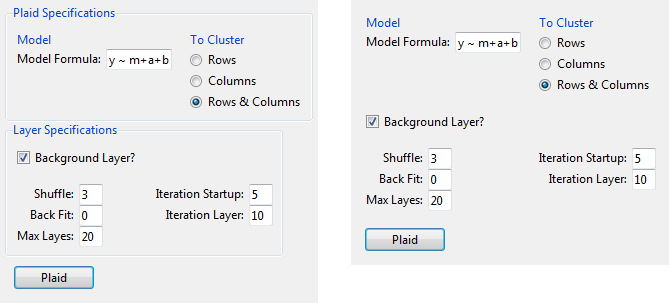
\includegraphics[scale=0.4]{figures/combinerows_grid.png}
\caption{{\it Left:} Rows 1 and 2+3 were combined with boxes and titles ; {\it
Right:} No rows combined. Frames are stuck in a general grid and jump more to
the right instead of in a `local' grid in a row box \label{combinerows_grid}}
\end{figure}

\newpage
\noindent {\bf \underline{PlotDiag Tab}}\\
\noindent The clustering tab configuration is immediately followed by making
the second tab.
\begin{knitrout}
\definecolor{shadecolor}{rgb}{0.969, 0.969, 0.969}\color{fgcolor}\begin{kframe}
\begin{alltt}
\hlcom{####################################}
\hlcom{#### PLOTTING & DIAGNOSTICS TAB ####}
\hlcom{####################################}
\hlstd{\{} \hlcom{# ignore this bracket}

\hlstd{input} \hlkwb{<-} \hlstr{"plotdiagTab"}

\hlcom{### 1. ADDING THE FRAMES ###}

\hlcom{# Add frames here}

\hlcom{### 2. CONFIGURING THE GRID ###}

\hlstd{grid.config} \hlkwb{<-} \hlkwd{.grid.matrix}\hlstd{(}\hlkwc{input}\hlstd{=input,}\hlkwd{c}\hlstd{(}\hlstr{"frame5"}\hlstd{,}\hlstr{"frame6"}\hlstd{),}\hlkwc{nrow}\hlstd{=}\hlnum{1}\hlstd{,}\hlkwc{ncol}\hlstd{=}\hlnum{2}\hlstd{,}
   \hlkwc{byrow}\hlstd{=}\hlnum{TRUE}\hlstd{,}\hlkwc{grid.config}\hlstd{=grid.config)}

\hlcom{### 3. COMBING THE ROWS ###}

\hlstd{grid.rows} \hlkwb{<-} \hlkwd{.combine.rows}\hlstd{(}\hlkwc{input}\hlstd{=input,}\hlkwc{rows}\hlstd{=}\hlkwd{c}\hlstd{(}\hlnum{1}\hlstd{),}\hlkwc{title}\hlstd{=}\hlstr{"Plot 1"}\hlstd{,}\hlkwc{border}\hlstd{=}\hlnum{TRUE}\hlstd{,}
   \hlkwc{grid.rows}\hlstd{=grid.rows,}\hlkwc{grid.config}\hlstd{=grid.config)}

\hlcom{###################################################################}
\hlcom{## USE ALL THE ARGUMENTS IN THE GENERAL CLUSTERTEMPLATE FUNCTION ##}
\hlcom{###################################################################}

\hlkwd{cluster_template}\hlstd{(}\hlkwc{methodname}\hlstd{=methodname,}\hlkwc{methodfunction}\hlstd{=methodfunction,}
   \hlkwc{methodhelp}\hlstd{=methodhelp,}\hlkwc{data.arg}\hlstd{=data.arg,}\hlkwc{other.arg}\hlstd{=other.arg,}
   \hlkwc{methodseed}\hlstd{=methodseed,}\hlkwc{grid.config}\hlstd{=grid.config,}\hlkwc{grid.rows}\hlstd{=grid.rows,}
   \hlkwc{new.frames}\hlstd{=new.frames,}\hlkwc{superbiclust.comp}\hlstd{=superbiclust.comp,}
   \hlkwc{bcdiag.comp}\hlstd{=bcdiag.comp,}\hlkwc{data.transf}\hlstd{=data.transf,}
   \hlkwc{data.discr}\hlstd{=data.discr,}\hlkwc{data.bin}\hlstd{=data.bin,}\hlkwc{methodshow}\hlstd{=methodshow,}
   \hlkwc{methodsave}\hlstd{=methodsave)}
\hlstd{\}}
\end{alltt}
\end{kframe}
\end{knitrout}

\noindent Analogous to the first tab, this part of the script starts by
putting the \verb|input| variable to {\it plotdiagTab}. Next the same three
steps are repeated as for the clustering tab. There is only one difference and
that is the addition of one new type of frame which can be created in the plots
\& diagnostics tab.
This is the {\it manual button frame} which will also be explained in more
detail down below. Basically a manual button can serve two purposes, it can be
tied to a plot or diagnostics function which uses some arguments (and then
create a graph) or it can lead to a new window entirely which can be created
with the {\it new tool script}.\\
Finally at the end of the script, all the variables and created objects are used
in the \verb|cluster_template| function which will create the actual window.
\\ \\
This \verb|cluster_template| call is the final line of the function
\verb|newmethod_WINDOW| we started creating in Section
\ref{sec:newmethodscript}. It is now ready to be used by R Commander to be
called upon as a window.

\subsubsection{The Frame Scripts}
In this section, the several types of frames which can be used in the
\verb|newmethod_script| will be showcased. The idea is that these parts of the
R-code (which are also in the Appendix) are copy-pasted into the
\verb|newmethod_script| and are adjusted as deemed necessary. \\
All the frame types have the \verb|title| and
\verb|border| option in common. The results of these options can be seen in
figure \ref{titleborder}. Also note that for each frametype the information is saved in
one object, namely \verb|new.frames|. Just as the grid and row configuration
earlier, new information will keep on getting added to this object, now with
the help of the \verb|.add.frame| function. Lastly, at the start of each frame
script, a \verb|type| variable will be set to determine the type of frame for
this previous mentioned \verb|.add.frame| function.

\begin{figure}[H]
\centering
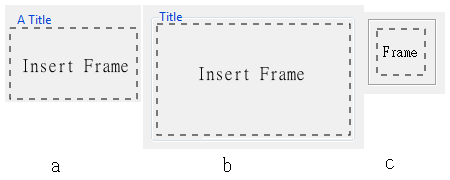
\includegraphics[scale=0.5]{figures/title_border.png}
\caption{{\bf a.}{\it Title \& No Border} {\bf b.}{\it Title \& Border} {\bf
c.}{\it No Title \& Border}
\label{titleborder}}
\end{figure}


\noindent {\bf Entry Fields}\\
\noindent The first type of frame is the entry fields frame. It can be used for
both numerical arguments and character arguments of your biclustering function.
Multiple entries can be added in one frame which will be placed below each
other.
\begin{figure}[H]
\centering
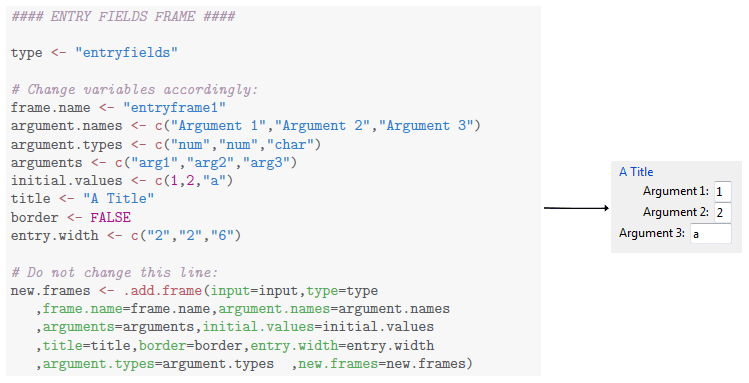
\includegraphics[scale=0.5]{figures/entryfields.png}
\caption{{\it Entry Fields: Code + Example}
\label{entryfields}}
\end{figure}

\noindent {\it Entry Fields Variables:}
\begin{description}
  \item[$\bullet$ \texttt{frame.name}:] The unique name of this frame. (Which is used in the grid matrix)
  \item[$\bullet$ \texttt{argument.names}:] The argument names how they will
  appear in the window.
  \item[$\bullet$ \texttt{argument.types}:] A vector defining if the argument is
  \verb|"num"| or \verb|"char"|. This basically just means if there should be a
  ' ' around the value when filling it in in the biclustering function. (e.g. In
  Figure \ref{entryfields} the arguments would be filled in as \verb|,arg1=1,arg2=2,arg3='a'|)
  \item[$\bullet$ \texttt{arguments}:] The actual argument names, used for the
  biclustering function.
  \item[$\bullet$ \texttt{initial.values}:] A vector containing the initial
  values in the entry fields.
  \item[$\bullet$ \texttt{title}:] Optional title for the frame (\verb|""| means no title)
  \item[$\bullet$ \texttt{border}:] Logical value determining the presence. 
  \item[$\bullet$ \texttt{entry.width}:] A vector containing the width of the
  entry fields (1 width = 1 number/character).
\end{description}

%\vspace{0.5cm}
\noindent {\bf Check Boxes}\\
The second type of frame is the check boxes frame which is used for
\verb|TRUE|/\verb|FALSE| arguments. Just like for entry fields, multiple check
boxes can be added below each other. 
\begin{figure}[H]
\centering
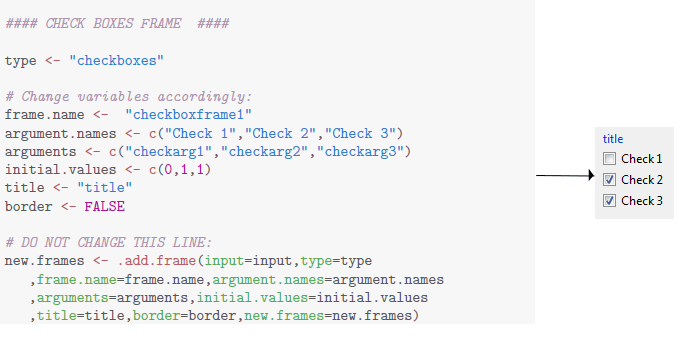
\includegraphics[scale=0.5]{figures/checkboxes.png}
\caption{{\it Check Boxes: Code + Example}
\label{checkboxes}}
\end{figure}

\noindent {\it Check Boxes Variables:}
\begin{description}
  \item[$\bullet$ \texttt{frame.name}:] The unique name of this frame. (Which is used in the grid matrix)
  \item[$\bullet$ \texttt{argument.names}:] The argument names how they will
  appear in the window.
  \item[$\bullet$ \texttt{arguments}:] The actual argument names, used for the
  biclustering function.
  \item[$\bullet$ \texttt{initial.values}:] A vector containing the initial
  values in the entry fields. (0 for \verb|FALSE|, 1 for \verb|TRUE|)
  \item[$\bullet$ \texttt{title}:] Optional title for the frame (\verb|""| means no title)
  \item[$\bullet$ \texttt{border}:] Logical value determining the presence. 
\end{description}


\noindent {\bf Radio Buttons}\\
The next type is radio buttons, which is used for only one argument with a
finite number of values.
\begin{figure}[H]
\centering
\includegraphics[scale=0.5]{figures/radiobuttons.png}
\caption{{\it Radio Buttons: Code + Example}
\label{radiobuttons}}
\end{figure}

\noindent {\it Radio Buttons Variables:}
\begin{description}
  \item[$\bullet$ \texttt{frame.name}:] The unique name of this frame. (Which is used in the grid matrix)
  \item[$\bullet$ \texttt{argument.names}:] The names of the buttons how they
  will appear in the window.
  \item[$\bullet$ \texttt{arguments}:] The actual argument name, used for the
  biclustering function.
  \item[$\bullet$ \texttt{argument.types}:] Just as for the entry fields, this
  will determine of the values are filled in with or without ''. The two options
  are again \verb|"num"| and \verb|"char"|, but in contrast with the entry
  fields it is now only one value and not a vector..
  \item[$\bullet$ \texttt{argument.values}:] The actual values of the radio buttons 
that correspond to the values passed to biclustering function. 
    \item[$\bullet$ \texttt{initial.values}:] The initial value of the radio
  buttons. It will determine which button is selected on opening the window.
  \item[$\bullet$ \texttt{title}:] Optional title for the frame (\verb|""| means no title)
  \item[$\bullet$ \texttt{border}:] Logical value determining the presence.   

\end{description}

\noindent {\bf Value Sliders}\\
The following type will create value sliders which can only be used for
numerical values. Again multiple sliders can be placed under each other. The
current value of the slider will always appear on top of it.

\begin{figure}[H]
\centering
\includegraphics[scale=0.5]{figures/slider.png}
\caption{{\it Value Slider: Code + Example}
\label{radiobuttons}}
\end{figure}

\noindent {\it Value Sliders Variables:}
\begin{description}
  \item[$\bullet$ \texttt{frame.name}:] The unique name of this frame. (Which is used in the grid matrix)
  \item[$\bullet$ \texttt{argument.names}:] The argument names how they will
  appear in the window.  
  \item[$\bullet$ \texttt{arguments}:] The actual argument names, used for the
  biclustering function.  
  \item[$\bullet$ \texttt{initial.values}:] Vector of initial values of the
  sliders.
  \item[$\bullet$ \texttt{from}:] Vector of starting points of the sliders.
  \item[$\bullet$ \texttt{to}:] Vector of ending points of the sliders.
  \item[$\bullet$ \texttt{by}:] Vector with the values determining how one
  movement of the sliders will change the current value.
  \item[$\bullet$ \texttt{length}:] Vector containing the lengths of the
  sliders.
  \item[$\bullet$ \texttt{title}:] Optional title for the frame (\verb|""| means no title)
  \item[$\bullet$ \texttt{border}:] Logical value determining the presence.   
  
\end{description}


\noindent {\bf Spin Boxes}\\
This type will create spin boxes which are again solely used for numerical
values. Just as for sliders, multiple spin boxes can be placed below each other.

\begin{figure}[H]
\centering
\includegraphics[scale=0.5]{figures/spinboxes.png}
\caption{{\it Spin Boxes: Code + Example}
\label{spinboxes}}
\end{figure}

\noindent {\it Spin Boxes Variables:}
\begin{description}
  \item[$\bullet$ \texttt{frame.name}:] The unique name of this frame. (Which is used in the grid matrix)
  \item[$\bullet$ \texttt{argument.names}:] The argument names how they will
  appear in the window.  
  \item[$\bullet$ \texttt{arguments}:] The actual argument names, used for the
  biclustering function.  
  \item[$\bullet$ \texttt{initial.values}:] Vector of initial values of the
  spin boxes.
  \item[$\bullet$ \texttt{from}:] Vector of starting points of the spin boxes.
  \item[$\bullet$ \texttt{to}:] Vector of ending points of the spin boxes.
  \item[$\bullet$ \texttt{by}:] Vector with the values determining how much one
  click will change the current value.
  \item[$\bullet$ \texttt{entry.width}:] Width of all the spinboxes (one value
  which applies to all of them)
  \item[$\bullet$ \texttt{title}:] Optional title for the frame (\verb|""| means no title)
  \item[$\bullet$ \texttt{border}:] Logical value determining the presence.   
  
\end{description}

\noindent {\bf Manual Buttons}\\
The last type of frame which can be utilized, is making manual buttons which
will {\it only} work in the plot \& diagnostics tab. As already explained
earlier, there are two primary uses for these buttons. The first use is to
simple execute a plot or diagnostic function, based on the arguments of other frames in
the window. The second application is to tie the button to another window
function (created with \verb|newtool_script|) to open up more options.

\begin{figure}[H]
\centering
\includegraphics[scale=0.5]{figures/manualbutton.png}
\caption{{\it Manual Button: Code + Example}
\label{manualbutton}}
\end{figure}

\noindent {\it Manual Button Variables:}
\begin{description}
  \item[$\bullet$ \texttt{frame.name}:] The unique name of this frame. (Which is used in the grid matrix)
  \item[$\bullet$ \texttt{button.name}:] The text which will appear on the
  button. No special characters are allowed and if the result of the button is
  saved, it will be in an object with this name without the spaces.
  \item[$\bullet$ \texttt{button.function}:] A string of the function which
  should be tied to this button. This could either be a plot, diagnostic or
  simple summary. Another useful practice is to actually make an entire
  new function for this manual button. This new function could then for
  example contain a series of diagnostic functions which would then be carried
  out all at the same time when clicking on this button.
  \item[$\bullet$ \texttt{button.data}:] The name of the data argument the
  button function. The data which is loaded in R Commander will then be
  pasted after this argument. (Simply put \verb|""| when this is not necessary)
  \item[$\bullet$ \texttt{button.biclust}:] The name of the biclustering result
  argument in the button function. Here the saved result after using the {\it
  Show Results} button will be pasted.
  \item[$\bullet$ \texttt{button.width}:] Character containing the width of the
  button. (Default = \verb|"12"|)
  \item[$\bullet$ \texttt{button.data.transf}:] Character determining if the
  data for \verb|button.data| should be transformed. (Values: \verb|"matrix"|
  (default), \verb|"ExprSet"|)
  \item[$\bullet$ \texttt{button.otherarg}:] Just like for the biclustering
  function (\verb|other.arg|), this is the variable in which one can add arguments to the
  function which should not be controlled by the user (e.g.
  \verb|",type='biclust'"|). Again, do not forget to add a comma in the
  beginning. 
  %The only time when the comma should be excluded is when both
  %\verb|button.data| and \verb|button.biclust| are put to \verb|""|.
  \item[$\bullet$ \texttt{arg.frames}:] A vector containing the names of those
  frames from which this button function should pull its arguments.
  \item[$\bullet$ \texttt{save}:] Logical value determining if the result of the
  button function should be saved. For example for a plotting function this is
  mosty likely not necessary, however for a diagnostic result it is. The
  difference between a \verb|TRUE| and \verb|FALSE| option is shown in figure
  \ref{manualbutton_showsave}.
  \item[$\bullet$ \texttt{show}:] Logical value determining if the button
  function should be shown in R Commander. It is good practice to do this for
  the plotting and diagnostics functions however if is a function to create a
  new window, it is probably not necessary to show it.

\end{description}


\begin{figure}[H]
\centering
\includegraphics[scale=0.5]{figures/manualbutton_showsave.png}
\caption{{\it Manual Buttons - save option}
\label{manualbutton_showsave}}
\end{figure}
%don't forget to say it is saved in new.frames
% idea to copy paste these in the script
% show without anything in it, the differnce beweetn, title, border etc

%show script + example plot
%explain script
%manualbuttons only for plotdiagtab!
%plotdiagtab: show/save options ; good idea to combine several functions in 1 buttonfunction (for diagnostic steps)

\subsubsection{A quick example - Plaid}
The entire script to construct the {\it Plaid Window} can be found in the
Appendix. In this small section, some parts will be highlighted and explained in
their context.
\begin{knitrout}
\definecolor{shadecolor}{rgb}{0.969, 0.969, 0.969}\color{fgcolor}\begin{kframe}
\begin{alltt}
\hlcom{#####################################################}
\hlcom{## GENERAL INFORMATION ABOUT THE NEW METHOD/WINDOW ##}
\hlcom{#####################################################}

\hlstd{methodname} \hlkwb{<-} \hlstr{"Plaid"}
\hlstd{methodfunction} \hlkwb{<-} \hlstr{"biclust"}
\hlstd{data.arg} \hlkwb{<-} \hlstr{"x"}
\hlstd{other.arg} \hlkwb{<-} \hlstr{",method=BCPlaid()"}
\hlstd{methodhelp} \hlkwb{<-} \hlstr{"BCPlaid"}
\hlstd{methodseed} \hlkwb{<-} \hlnum{TRUE}
\hlstd{data.discr} \hlkwb{<-} \hlnum{FALSE}
\hlstd{data.bin} \hlkwb{<-} \hlnum{FALSE}
\hlstd{bcdiag.comp} \hlkwb{<-} \hlnum{TRUE}
\hlstd{superbiclust.comp} \hlkwb{<-} \hlnum{TRUE}

\hlcom{# Biclust only (Not for public use)}
\hlstd{extrabiclustplot} \hlkwb{<-} \hlnum{TRUE}
\end{alltt}
\end{kframe}
\end{knitrout}
\noindent First of all, the general information is filled in for the plaid
method as shown in the script above. Please note that the
\verb|extrabiclustplot| is a \verb|biclust|-only variable and will not be elaborated on.
\\ \\
Next, in Figure \ref{plaid_clusterbuild} we can see the code which makes the two
frames in the top row.
\begin{figure}[H]
\centering
\includegraphics[scale=0.45]{figures/plaid_clusterbuild.png}
\caption{{\it Building the Plaid Window - ClusterTab}
\label{plaid_clusterbuild}}
\end{figure}

\noindent After adding the frame scripts, the next step is the grid
configuring and the row combining of the cluster tab. In this extract of the
script, one can see the two frames from Figure \ref{plaid_clusterbuild} being
placed in the top row of the matrix after which the first row is made into a box
with border and {\it Plaid Specifications} title.
\begin{knitrout}
\definecolor{shadecolor}{rgb}{0.969, 0.969, 0.969}\color{fgcolor}\begin{kframe}
\begin{alltt}
\hlcom{### 2. CONFIGURING THE GRID ###}
\hlstd{grid.config} \hlkwb{<-} \hlkwd{.grid.matrix}\hlstd{(}\hlkwc{input}\hlstd{=input,}\hlkwd{c}\hlstd{(}\hlstr{"toclusterframe"}\hlstd{,}\hlstr{"modelframe"}\hlstd{,}
   \hlstr{"backgroundcheckframe"}\hlstd{,}\hlnum{NA}\hlstd{,}\hlstr{"backgroundentryframe1"}\hlstd{,}\hlstr{"backgroundentryframe2"}\hlstd{),}
   \hlkwc{byrow}\hlstd{=}\hlnum{TRUE}\hlstd{,}\hlkwc{nrow}\hlstd{=}\hlnum{3}\hlstd{,}\hlkwc{ncol}\hlstd{=}\hlnum{2}\hlstd{,}\hlkwc{grid.config}\hlstd{=grid.config)}

\hlcom{### 3. COMBING THE ROWS ###}
\hlstd{grid.rows} \hlkwb{<-} \hlkwd{.combine.rows}\hlstd{(}\hlkwc{input}\hlstd{=input,}\hlkwc{rows}\hlstd{=}\hlkwd{c}\hlstd{(}\hlnum{1}\hlstd{),}\hlkwc{title}\hlstd{=}\hlstr{"Plaid Specifications"}\hlstd{,}
   \hlkwc{border}\hlstd{=}\hlnum{TRUE}\hlstd{,}\hlkwc{grid.rows}\hlstd{=grid.rows,}\hlkwc{grid.config}\hlstd{=grid.config)}
\hlstd{grid.rows} \hlkwb{<-} \hlkwd{.combine.rows}\hlstd{(}\hlkwc{input}\hlstd{=input,}\hlkwc{rows}\hlstd{=}\hlkwd{c}\hlstd{(}\hlnum{2}\hlstd{,}\hlnum{3}\hlstd{),}\hlkwc{title}\hlstd{=}\hlstr{"Layer Specifications"}\hlstd{,}
   \hlkwc{border}\hlstd{=}\hlnum{TRUE}\hlstd{,}\hlkwc{grid.rows}\hlstd{=grid.rows,}\hlkwc{grid.config}\hlstd{=grid.config)}
\end{alltt}
\end{kframe}
\end{knitrout}
\noindent Finally,  an example of the creation of manual
buttons is shown in Figure \ref{plaid_plotdiagbuild}. Note
that the line of code containing the \verb|.add.frame| has been omitted here
for better clarity of the code. The button here is tied to the function
\verb|"drawHeatmap"| and draws its arguments from \verb|"heatplotcheckframe"|
and \verb|"heatplotentryframe"| which are both defined in \verb|arg.frames|.\\
Naturally the creations of all the other frames, together with the configuring
of the grid and combining of the rows follows after.
\begin{figure}[H]
\centering
\includegraphics[scale=0.44]{figures/plaid_plotdiagbuild.png}
\caption{{\it Building the Plaid Window - PlotDiagTab}
\label{plaid_plotdiagbuild}}
\end{figure}


\subsection{Implementing a New Tool}
\noindent The second template script (which is also available in the Appendix)
is \verb|newtool_script.R|. With the help of this script one can make a new window
which can for example be tied to a manual button in the second tab of a
clustering window. Another possibility is to make another general diagnostics
window compatible with several other biclustering packages. This is for example
already done with the \verb|BcDiag| and \verb|superbiclust| package for which
the button appears in the second tab of the compatible methods.
Also just as for these two packages, a compatibility variable could then be
added in the begin of the \verb|newmethod_script| to decide if the button for your new
general diagnostics package should appear for a specific method.
% can be used for overhauling diagnostics AND making new windows tied to buttons
% bit more detail about general diagnostic, give BcDiag example
\subsubsection{New Tool Script}
\begin{knitrout}
\definecolor{shadecolor}{rgb}{0.969, 0.969, 0.969}\color{fgcolor}\begin{kframe}
\begin{alltt}
\hlstd{newtool_WINDOW} \hlkwb{<-} \hlkwa{function}\hlstd{(}\hlkwc{methodname}\hlstd{)\{}

        \hlstd{new.frames} \hlkwb{<-} \hlkwd{.initialize.new.frames}\hlstd{()}
        \hlstd{grid.config} \hlkwb{<-} \hlkwd{.initialize.grid.config}\hlstd{()}
        \hlstd{grid.rows} \hlkwb{<-} \hlkwd{.initialize.grid.rows}\hlstd{()}

        \hlcom{#####################################################}
        \hlcom{## GENERAL INFORMATION ABOUT THE NEW TOOL		   ##}
        \hlcom{#####################################################}

        \hlstd{toolname} \hlkwb{<-} \hlstr{"A new tool"}
        \hlstd{toolhelp} \hlkwb{<-} \hlstr{"helppage"}

        \hlcom{# Do not change this line:}
        \hlstd{input} \hlkwb{<-} \hlstr{"plotdiagTab"}

        \hlcom{### ADDING FRAMES ####}

        \hlcom{# Analogous to plotdiag tab.}

        \hlcom{### CONFIGURING GRID ###}
        \hlstd{grid.config} \hlkwb{<-} \hlkwd{.grid.matrix}\hlstd{(}\hlkwc{input}\hlstd{=input,}\hlkwd{c}\hlstd{(),}\hlkwc{nrow}\hlstd{=}\hlnum{1}\hlstd{,}\hlkwc{ncol}\hlstd{=}\hlnum{2}\hlstd{,}
           \hlkwc{byrow}\hlstd{=}\hlnum{TRUE}\hlstd{,}\hlkwc{grid.config}\hlstd{=grid.config)}


        \hlcom{### COMBINING ROWS ###}
        \hlstd{grid.rows} \hlkwb{<-} \hlkwd{.combine.rows}\hlstd{(}\hlkwc{input}\hlstd{=input,}\hlkwc{rows}\hlstd{=}\hlkwd{c}\hlstd{(),}\hlkwc{title}\hlstd{=}\hlstr{"Plot 1"}\hlstd{,}
           \hlkwc{border}\hlstd{=}\hlnum{TRUE}\hlstd{,}\hlkwc{grid.rows}\hlstd{=grid.rows,}\hlkwc{grid.config}\hlstd{=grid.config)}

        \hlcom{############################################################}
        \hlcom{## USE ALL THE ARGUMENTS IN THE GENERAL NEW TOOL FUNCTION ##}
        \hlcom{############################################################}

        \hlkwd{newtool_template}\hlstd{(}\hlkwc{toolname}\hlstd{=toolname,}\hlkwc{methodname}\hlstd{=methodname,}
           \hlkwc{toolhelp}\hlstd{=toolhelp,}\hlkwc{grid.config}\hlstd{=grid.config,}
           \hlkwc{grid.rows}\hlstd{=grid.rows,}\hlkwc{new.frames}\hlstd{=new.frames)}
\hlstd{\}}
\end{alltt}
\end{kframe}
\end{knitrout}
\noindent Just as for \verb|newmethod_script| the adjusting of the template
starts with changing \verb|newtool_WINDOW| to your own desired windowfunction
name. Next at the start of the script again the necessary objects are
initialized followed by some variables containing general information about the
tool:
\begin{description}
  \item[$\bullet$ \texttt{toolname}:] The name of the tool appearing at the top
  of the window. 
  \item[$\bullet$ \texttt{toolhelp}:] The helppage the help button should be
  linked with. (\verb|help(toolhelp)|)
\end{description}
\noindent After filling in these couple of variables, making this window is {\it
exactly} the same as creating the second tab in \verb|newmethod_script|. This
means it is also possible to create manual buttons in this window. Note that
even the \verb|input| variable is again set to {\it plotdiagTab}. The only
difference can be found in the last line where now the template function has
changed to \verb|newtool_template|.\\
Finally the attention should also be pointed to the fact that by default the
\verb|newtool_WINDOW| function has \verb|methodname| as an argument. This means
if this function is used inside a \verb|newmethod_script|, the new tool window
can behave differently depending on the method it is being called by. This will
become clear in the example shortly. 

\subsubsection{A quick example - BcDiag}
\noindent We will now go through a couple of parts of the script responsible for
the BcDiag window. The full script can once again be found in the Appendix.

\begin{knitrout}
\definecolor{shadecolor}{rgb}{0.969, 0.969, 0.969}\color{fgcolor}\begin{kframe}
\begin{alltt}
\hlstd{bcdiag_WINDOW} \hlkwb{<-} \hlkwa{function}\hlstd{(}\hlkwc{methodname}\hlstd{)\{}

        \hlstd{new.frames} \hlkwb{<-} \hlkwd{.initialize.new.frames}\hlstd{()}
        \hlstd{grid.config} \hlkwb{<-} \hlkwd{.initialize.grid.config}\hlstd{()}
        \hlstd{grid.rows} \hlkwb{<-} \hlkwd{.initialize.grid.rows}\hlstd{()}

        \hlcom{# Some extra code to determine the input type: "biclust", "fabia", "isa2"}
        \hlstd{biclust.names} \hlkwb{<-} \hlkwd{c}\hlstd{(}\hlstr{"Bimax"}\hlstd{,}\hlstr{"CC"}\hlstd{,}\hlstr{"Plaid"}\hlstd{,}\hlstr{"Questmotif"}\hlstd{,}\hlstr{"Spectral"}\hlstd{,}
           \hlstr{"XMotifs"}\hlstd{,}\hlstr{"IBBIG"}\hlstd{)}
        \hlstd{fabia.names} \hlkwb{<-} \hlkwd{c}\hlstd{(}\hlstr{"Fabia Laplace Prior"}\hlstd{,}\hlstr{"Fabia Post-Projection"}\hlstd{,}
            \hlstr{"Fabia Sparseness Projection"}\hlstd{,}\hlstr{"Fabia SPARSE"}\hlstd{)}
        \hlstd{isa.names} \hlkwb{<-} \hlkwd{c}\hlstd{(}\hlstr{"ISA"}\hlstd{)}

        \hlkwa{if}\hlstd{(methodname} \hlopt \hlstd{biclust.names)\{}
                \hlstd{extra.arg} \hlkwb{<-} \hlstr{",mname='biclust'"}
        \hlstd{\}}
        \hlkwa{if}\hlstd{(methodname} \hlopt \hlstd{fabia.names)\{}
                \hlstd{extra.arg} \hlkwb{<-} \hlstr{",mname='fabia'"}
        \hlstd{\}}
        \hlkwa{if}\hlstd{(methodname} \hlopt \hlstd{isa.names)\{}
                \hlstd{extra.arg} \hlkwb{<-} \hlstr{",mname='isa2'"}
        \hlstd{\}}

        \hlcom{#####################################################}
        \hlcom{## GENERAL INFORMATION ABOUT THE NEW TOOL		   ##}
        \hlcom{#####################################################}

        \hlstd{toolname} \hlkwb{<-} \hlstr{"BCDIAG"}
        \hlstd{toolhelp} \hlkwb{<-} \hlstr{"BcDiag-package"}

\hlstd{\}}\hlcom{#ignore}
\end{alltt}
\end{kframe}
\end{knitrout}
\noindent In the code above the variables containing the general information are
filled in as expected, however just above some extra code has been added. These
extra lines of code are simply determining what string should be saved in
\verb|extra.arg| based on the \verb|methodname| given to \verb|bcdiag_WINDOW|.
This \verb|extra.arg| variable will then be used later in the creation of a
manual button as we will see now in Figure \ref{bcdiag_build}. Note that just as
for the plaid example the \verb|.add.frame| line has been omitted to maintain
clarity.
\begin{figure}[H]
\centering
\includegraphics[scale=0.45]{figures/bcdiag_build.png}
\caption{{\it Building the BcDiag Window}
\label{bcdiag_build}}
\end{figure}
\noindent Apart from the usual framebuilding, one can see that this earlier
mentioned \verb|extra.arg| is now used for the \verb|button.otherarg| argument in the
manual button setup. \\
This is only one of many ways in which you can tailor the tool window to a
specific biclustering method. A more complicated example would the implementation of the
\verb|superbiclust| window in which \verb|methodname| is also transformed to
\verb|method_result| (\verb|methodname| without spaces and `-`'s) in order to
make some distinguishments. Further in this script a different
\verb|grid.config| and \verb|grid.rows| will be created depending on
\verb|methodname|.\\
Since apart from these additions the script is still very much the same as the
others, it will not be elaborated on. It can however still be found in the
Appendix.
\subsection{How to start?}
\noindent The easiest way to start making your own dialog, is to copy the
\verb|newmethod_script.R| (or \verb|newtool_script.R|) to your own file. Next,
simply change the variables so they fit your new application and add new frames
by copying and adapting the default ones from \verb|frames_scripts.R| inside your
new file. Note that all of the above mentioned R files are available in the documentation
folder of \verb|RcmdrPlugin.BiclustGUI|.
Finally, to test your new window, simply load in the BiclustGUI in R and
run the \verb|newmethod_WINDOW| function you've created.

% give some explanation of method_result
%explain the bit of code in the beginning ( to decide the button.other variables)
% rest of construction similar to already seen
% full code, see script
% for more complicated example -> superbiclust
\section{Extensions - Shiny App \& \texttt{REST}}
The main functionality of the \texttt{BiclustGUI} was also recreated in the form of a Shiny Application. The \texttt{shiny} R package \citep{Chang2015}, developed by RStudio, allows the creation of web-based applications from R-code. Shiny Apps are very accessible since they do not require any installation on the user side. They can be hosted on a private website, Shiny Cloud and also Amazon Cloud. It also possible to distribute them in a stand-alone version. The Shiny Apps are often highly interactive due to the use of reactive functions, allowing the App to immediately adapt to any input of the user. The \texttt{shiny} R package, provides a large amount of basic widgets, i.e. web elements users can interact with, of which some are built using the Bootstrap Project. Note that compared to the \texttt{BiclustGUI} in R Commander, the user will not shown the generated R on the fly.\\
The biclustGUI Shiny App can found at \href{ewouddetroyer.shinyapps.io/shiny-biclust}{ewouddetroyer.shinyapps.io/shiny-biclust}. It is also available as a stand-alone version to run locally on your pc at \href{http://www.xxxxxx}{http://www.xxxxxx}. Simply extract the zip-file and double click the \texttt{LAUNCH.vbs} file (no installation, e.g. R, required!).
\begin{figure}[H]
\centering
\includegraphics[width=0.45\textwidth]{figures/shinyibbig.png}
\caption{Shiny Example (iBBiG) - Biclusters Heatmap}\label{fig:shinyibbig}
\end{figure}
\noindent The template scripts for biclustering windows were also the foundations for the \texttt{REST} package \citep{DeTroyer2015}. 
With this package, it is possible to create plug-ins for R Commander without expert knowledge, providing a tool to 
create envelope GUI packages similar to \texttt{BiclustGUI}.\\ \\
The \texttt{REST} package ({\bf R}mdrPlugin {\bf E}asy {\bf S}cript {\bf T}emplates) 
contains a generalization of the biclustering window scripts. These scripts, previously tailored towards a 
window structure for the biclustering dialogs, are now more general and flexible (i.e. allowing more tabs, more buttons,etc.).\\
The \texttt{REST} package allows a fast and easy creation of a R Commander
plug-in without the \texttt{tcltk} syntax, can be used to create the windows for
a new applications, and is freely available on CRAN with \texttt{install.packages("REST")} (Dependencies: \texttt{Rcmdr}).\\
The \texttt{REST} package also contains a vignette similar to Section
\ref{sec:guideline} of this vignette. The guide is more general in its
construction of a GUI window, but also contains some extra explanation and
specializations.

\newpage
\nocite{*}
\bibliographystyle{asa}
\bibliography{ThesisBiclustGUIbib}


\newpage
\section{Appendix}
\subsection{Introduction}
\begin{figure}[H]
\centering
\includegraphics[scale=0.25]{figures/bicluster_types.png}
\caption{{\it Several Types of Biclusters}\label{bicluster_types}}
\end{figure}
\begin{figure}[H]
\centering
\includegraphics[scale=0.2]{figures/bicluster_structures.png}
\caption{{\it Underlying Bicluster Structures}\label{bicluster_structures}}
\end{figure}
\subsection{The BiclustGUI R Package}
\subsubsection{Installing and Loading - Installing Script}
\begin{verbatim}
## PACKAGES AVAILABLE ON CRAN ##
install.packages("biclust")
install.packages("BcDiag")
install.packages("superbiclust")
install.packages("Rcmdr")
install.packages("isa2")

install.packages("gplots") # Extra package

## PACKAGES AVAILABLE ON BIOCONDUCTOR ##
source("http://bioconductor.org/biocLite.R")
biocLite("iBBiG")
biocLite("fabia")
biocLite("rqubic")
biocLite("BicARE")

## Biclust GUI - Development Version ##
install.packages("RcmdrPlugin.BiclustGUI", 
repos="http://R-Forge.R-project.org")

## Biclust GUI - Release Version  ##
install.packages("RcmdrPlugin.BiclustGUI")

\end{verbatim}

\subsubsection{Extra Utilities}

\begin{figure}[H]
\centering
\includegraphics[scale=0.33]{figures/drawheatmaps_example1.png}
\caption{{\it Data Heatmap - Normal \& Binary }\label{drawheatmaps_example1}}
\end{figure}
\begin{figure}[H]
\centering
\includegraphics[scale=0.33]{figures/drawheatmaps_example2.png}
\caption{{\it Result Heatmap - Default \& Reordered with Background
}\label{drawheatmaps_example2}}
\end{figure}


\subsubsection{\texttt{biclust}-package}
\begin{figure}[H]
\centering
\includegraphics[scale=0.4]{figures/biclustplot_example1.png}
\caption{{\it An example of bootstrap output \&
Histograms}\label{biclustplot_example1}}
\end{figure}
\begin{figure}[H]
\centering
\includegraphics[scale=0.4]{figures/biclustplot_example2.png}
\caption{{\it An example of Parallel Coordinates
Plot - Default Type (row \& column $+$ Compare) \&
Combined Type}\label{biclustplot_example2}}
\end{figure}
\begin{figure}[H]
\centering
\includegraphics[scale=0.4]{figures/biclustplot_example3.png}
\caption{{\it An example of the Heatmap - Local \&
Full Matrix}\label{biclustplot_example3}}
\end{figure}
\begin{figure}[H]
\centering
\includegraphics[scale=0.4]{figures/biclustplot_example4.png}
\caption{{\it An example of BiclustMember Plot -
Mid Checked \& Mid Unchecked}\label{biclustplot_example4}}
\end{figure}
\begin{figure}[H]
\centering
\includegraphics[scale=0.4]{figures/biclustplot_example5.png}
\caption{{\it An example of Biclust Bubble Plot
with Mean Projection}\label{biclustplot_example5}}
\end{figure}
\begin{figure}[H]
\centering
\includegraphics[scale=0.4]{figures/biclustplot_example6.png}
\caption{{\it An example of the Barplots}\label{biclustplot_example6}}
\end{figure}
\begin{figure}[H]
\centering
\includegraphics[scale=0.4]{figures/biclustplot_example7.png}
\caption{{\it An example of Bicluster Barchart}\label{biclustplot_example7}}
\end{figure}
\subsubsection{\texttt{fabia}-package}
\begin{figure}[H]
\centering
\includegraphics[scale=0.4]{figures/fabiaplot_example1.png}
\caption{{\it Examples of Information Content
Histogram of biclusters and samples}\label{fabiaplot_example1}}
\end{figure}
\begin{figure}[H]
\centering
\includegraphics[scale=0.4]{figures/fabiaplot_example2.png}
\caption{{\it Examples of boxplots of Loadings \&
Factors}\label{fabiaplot_example2}}
\end{figure}
\begin{figure}[H]
\centering
\includegraphics[scale=0.3]{figures/fabiaplot_example3.png}
\caption{{\it Examples Extract Plots}\label{fabiaplot_example3}}
\end{figure}
\begin{figure}[H]
\centering
\includegraphics[scale=0.4]{figures/fabiaplot_example4.png}
\caption{{\it Example of Bicluster Plot - Full \&
Only Bicluster}\label{fabiaplot_example4}}
\end{figure}
\begin{figure}[H]
\centering
\includegraphics[scale=0.4]{figures/fabiaplot_example5.png}
\caption{{\it Example of BiPlot}\label{fabiaplot_example5}}
\end{figure}

\subsubsection{\texttt{isa2}-package}
\begin{figure}[H]
\centering
\includegraphics[scale=0.3]{figures/isa_example1.png}
\caption{{\it An example of score \& module plot}\label{isa_example1}}
\end{figure}

\subsubsection{\texttt{iBBiG}-package}
\begin{figure}[H]
\centering
\includegraphics[scale=0.5]{figures/ibbig_example1.png}
\caption{{\it An example of the general iBBiG plot}\label{ibbig_example1}}
\end{figure}

\subsubsection{\texttt{BicARE}-package}
\begin{figure}[H]
\centering
\includegraphics[scale=0.4]{figures/bicare_example1.png}
\caption{{\it Example of Residue Plot}\label{bicare_example1}}
\end{figure}
\begin{figure}[H]
\centering
\includegraphics[scale=0.4]{figures/bicare_example2.png}
\caption{{\it Example of Extract Bicluster Plot}\label{bicare_example2}}
\end{figure}
\begin{figure}[H]
\centering
\includegraphics[scale=0.4]{figures/bicare_example3.png}
\caption{{\it Example of the homepage of `Make Report'}\label{bicare_example3}}
\end{figure}

\subsubsection{\texttt{BcDiag}-package}
\begin{figure}[H]
\centering
\includegraphics[scale=0.25]{figures/bcdiag_example1.png}
\caption{{\it ANOVA \& Residual Plots: Diagnostic Plots and ANOVA \& Mpolish
}\label{bcdiag_example1}}
\end{figure}
\begin{figure}[H]
\centering
\includegraphics[scale=0.25]{figures/bcdiag_example2.png}
\caption{{\it Profile Plots: Example of all types for gene \& condition
dimension }\label{bcdiag_example2}}
\end{figure}
\begin{figure}[H]
\centering
\includegraphics[scale=0.25]{figures/bcdiag_example3.png}
\caption{{\it Exploratory Plots: Left and right button
for gene dimension}\label{bcdiag_example3}}
\end{figure}
\subsubsection{\texttt{superbiclust}-package}
\begin{figure}[H]
\centering
\includegraphics[scale=0.5]{figures/superbiclust_example1.png}
\caption{{\it Example of a superbiclust tree (Note that this tree is only here
for example purposes. All the biclusters here seem to be unique.)}\label{superbiclust_example1}}
\end{figure}
\begin{figure}[H]
\centering
\includegraphics[scale=0.5]{figures/superbiclust_example2.png}
\caption{{\it Example of Robust BC button with Show Inside
checked}\label{superbiclust_example2}}
\end{figure}

\subsection{Guideline - Template Scripts}
\subsubsection{newmethod\_script}
\noindent This script can also be found in the \verb|doc| subdirectory of the
package.
\begin{verbatim}
newmethod_WINDOW <- function(){     # Change newmethod to your own method name
	
	new.frames <- .initialize.new.frames()
	grid.config <- .initialize.grid.config()
	grid.rows <- .initialize.grid.rows()
	
	
	#####################################################
	## GENERAL INFORMATION ABOUT THE NEW METHOD/WINDOW ##
	#####################################################

	methodname <- "A new method"

	methodfunction <- "methodfunction"
	data.arg <- "d"
	methodshow <- TRUE
	other.arg <- ""
	methodhelp <- ""

	# Transform the data from data.arg
	data.transf <- "matrix" # Values: "matrix" (default), "ExprSet"

	# Extra Data Conversion Boxes
	data.discr <- FALSE
	data.bin <- FALSE
		
	# Possibility to give a seed ?
	methodseed <- TRUE
	
	## COMPATIBILITY? ##
	
	# BcDiag
	bcdiag.comp <- FALSE
	
	# SuperBiclust
	superbiclust.comp <- FALSE
	
		
	########################
	#### CLUSTERING TAB ####
	########################
	
	input <- "clusterTab"
	
	### 1. ADDING THE FRAMES ###
	
	# Add frames here
	
	### 2. CONFIGURING THE GRID ###
	
	grid.config <- .grid.matrix(input=input,c("frame1","frame2","frame3",NA
    ,"frame4",NA),nrow=3,ncol=2,byrow=TRUE,grid.config=grid.config)
	
	
	### 3. COMBING THE ROWS ###

	grid.rows <- .combine.rows(input=input,rows=c(1),title="A nice box: "
    ,border=TRUE,grid.rows=grid.rows,grid.config=grid.config)
	grid.rows <- .combine.rows(input=input,rows=c(2,3),title="A nice box: "
    ,border=TRUE,grid.rows=grid.rows,grid.config=grid.config)
	
	
	
	####################################
	#### PLOTTING & DIAGNOSTICS TAB ####
	####################################
	
	input <- "plotdiagTab"
		
	### 1. ADDING THE FRAMES ###
	
	# Add frames here
	
	### 2. CONFIGURING THE GRID ###
	
	grid.config <- .grid.matrix(input=input,c("frame5","frame6"),nrow=1,
    ncol=2,byrow=TRUE,grid.config=grid.config)
		
	### 3. COMBING THE ROWS ###
	
	grid.rows <- .combine.rows(input=input,rows=c(1),title="Plot 1",
    border=TRUE,grid.rows=grid.rows,grid.config=grid.config)
		
	###################################################################
	## USE ALL THE ARGUMENTS IN THE GENERAL CLUSTERTEMPLATE FUNCTION ##
	###################################################################
	
	cluster_template(methodname=methodname,methodfunction=methodfunction,
    methodhelp=methodhelp,data.arg=data.arg,other.arg=other.arg
    ,methodseed=methodseed,grid.config=grid.config,grid.rows=grid.rows,
    new.frames=new.frames,superbiclust.comp=superbiclust.comp,
    bcdiag.comp=bcdiag.comp,data.transf=data.transf,
    data.discr=data.discr, data.bin=data.bin,methodshow=methodshow,
    methodsave=methodsave)
	
}
\end{verbatim}
\subsubsection{frames\_script}
\begin{verbatim}
#### ENTRY FIELDS FRAME ####

type <- "entryfields"

# Change variables accordingly:
frame.name <- "entryframe1"  
argument.names <- c("Argument 1","Argument 2","Argument 3") 
argument.types <- c("num","num","char") 
arguments <- c("arg1","arg2","arg3") 
initial.values <- c(1,2,"a")
title <- "A Title"
border <- FALSE
entry.width <- c("2","2","6")

# Do not change this line:
new.frames <- .add.frame(input=input,type=type
    ,frame.name=frame.name,argument.names=argument.names
    ,arguments=arguments,initial.values=initial.values
    ,title=title,border=border,entry.width=entry.width
    ,argument.types=argument.types  ,new.frames=new.frames)




#### RADIO BUTTONS FRAME 	####

type <- "radiobuttons"

# Change variables accordingly:
frame.name <- "radioframe1"
argument.names <- c("Button 1","Button 2","Button 3")  
arguments <- c("buttonarg")		
argument.types <- "char" 
argument.values <- c("b1","b2","b3") 
initial.values <- "b3"
title <- "Button Options"
border <- TRUE

# DO NOT CHANGE THIS LINE:
new.frames <- .add.frame(input=input,type=type
    ,frame.name=frame.name,argument.names=argument.names
    ,arguments=arguments,argument.values=argument.values
    ,initial.values=initial.values,title=title,border=border
    ,new.frames=new.frames,argument.types=argument.types)	


#### CHECK BOXES FRAME  ####

type <- "checkboxes"

# Change variables accordingly:
frame.name <-  "checkboxframe1"
argument.names <- c("Check 1","Check 2","Check 3")  
arguments <- c("checkarg1","checkarg2","checkarg3") 
initial.values <- c(0,1,1)  
title <- "title"
border <- FALSE

# DO NOT CHANGE THIS LINE:
new.frames <- .add.frame(input=input,type=type
    ,frame.name=frame.name,argument.names=argument.names
    ,arguments=arguments,initial.values=initial.values
    ,title=title,border=border,new.frames=new.frames)


#### VALUE SLIDER FRAME  ####

type <- "valuesliders"

# Change variables accordingly:
frame.name <- "sliderframe1"
argument.names <- c("Slider 1  ","Slider 2  ","Slider 3  ")
arguments <- c("sliderarg1","sliderarg2","sliderarg3") 
initial.values <- c(1,5,10)
from <- c(1,1,1) 
to <- c(5,50,500) 
by <- c(1,10,50)  
length <- c(50,100,150) 
title <- "Title"
border <- TRUE

# DO NOT CHANGE THIS LINE:
new.frames <- .add.frame(input=input,type=type,
    title=title,border=border,frame.name=frame.name,
    argument.names=argument.names,arguments=arguments,
    initial.values=initial.values,from=from,to=to,by=by,
    length=length,new.frames=new.frames)


#### SPIN BOX FRAME  ####

type <- "spinboxes"

# Change variables accordingly:
frame.name <- "spinboxframe1"
argument.names <- c("Spin Box 1: ","Spin Box 2: ","Spin Box 3: ") 
arguments <- c("spinarg1","spingarg2","spingarg3") 
initial.values <- c(5,10,20)
from <- c(1,5,10)  
to <- c(10,20,30)
by <- c(1,1,1)
entry.width <- "2"  
title <- "Spin Box !"
border <- TRUE

# DO NOT CHANGE THIS LINE:
new.frames <- .add.frame(input=input,type=type,
    frame.name=frame.name,argument.names=argument.names,
    arguments=arguments,initial.values=initial.values,
    from=from,to=to,by=by,entry.width=entry.width,
    title=title,border=border,new.frames=new.frames)


#### MANUAL BUTTONS FRAME ####

type <- "buttons"

# Change variables accordingly:
frame.name <- "buttonframe1"  
button.name <- "Button 1"  
button.function <- "buttonfunction" 
button.data <- "d" 
button.biclust <-  "biclust" 
button.width <- "12"
button.data.transf <- "matrix"

arg.frames <- c("frame1","frame2")

save <- TRUE 
show <- TRUE
button.otherarg <- "" 

# Do not change this line: 
new.frames <- .add.frame(input=input,frame.name=frame.name,
		type=type,button.name=button.name,
		button.function=button.function,button.data=button.data,
		button.biclust=button.biclust,button.otherarg=button.otherarg,
		button.width=button.width,button.data.transf=button.data.transf,
		arg.frames=arg.frames,save=save,show=show,new.frames=new.frames)


\end{verbatim}
\subsubsection{Quick Example - Plaid}
\begin{verbatim}
biclustplaid_WIN <- function(){     
	
	new.frames <- .initialize.new.frames()
	grid.config <- .initialize.grid.config()
	grid.rows <- .initialize.grid.rows()
		
	#####################################################
	## GENERAL INFORMATION ABOUT THE NEW METHOD/WINDOW ##
	#####################################################
	

	methodname <- "Plaid"
	methodfunction <- "biclust"
	data.arg <- "x"
	data.matrix <- TRUE
	other.arg <- ",method=BCPlaid()"   
	methodhelp <- "BCPlaid"
	
	# Possibility to give a seed ?
	methodseed <- TRUE
	# Add a discretize box?
	data.discr <- FALSE
	# Add a binarize box?
	data.bin <- FALSE
	
	## COMPATIBILITY? ##
	
	# BcDiag
	bcdiag.comp <- TRUE
	
	# SuperBiclust
	superbiclust.comp <- TRUE
	
	# Biclust only (Not for public use)
	extrabiclustplot <- TRUE
	
	########################
	#### CLUSTERING TAB ####
	########################
	
	### 1. ADDING THE FRAMES ###
	
	input <- "clusterTab"
	
	
	####		RADIO BUTTONS FRAME 		 ####
	
	type <- "radiobuttons"
	
	# Change variables accordingly:
	frame.name <- "toclusterframe"
	argument.names <- c("Rows","Columns","Rows & Columns")   
	arguments <- c("cluster")		
	argument.values <- c("r","c","b")
	argument.types <- "char"
	initial.values <- "b" 
	title <- "To Cluster"
	border <- FALSE
	
	# DO NOT CHANGE THIS LINE:
	new.frames <- .add.frame(input=input,type=type,
     frame.name=frame.name,argument.names=argument.names,
    arguments=arguments,argument.values=argument.values,
    initial.values=initial.values,title=title,border=border,
    new.frames=new.frames,argument.types=argument.types)	
	
	
	######		  ENTRY FIELDS FRAME 				#####
	
	type <- "entryfields"
	
	# Change variables accordingly:
	frame.name <- "modelframe"  
	argument.names <- c("Model Formula") 
	argument.types <- c("num")
	arguments <- c("fit.model")
	initial.values <- c("y ~ m+a+b")
	title <- "Model"
	border <- FALSE
	entry.width <- c("10")  
	
	# Do not change this line:
	new.frames <- .add.frame(input=input,type=type,frame.name=frame.name,
    argument.names=argument.names,arguments=arguments,initial.values=
    initial.values,title=title,border=border,entry.width=entry.width,
    argument.types=argument.types  ,new.frames=new.frames)
	
	####		CHECK BOXES FRAME 			  ####
	
	type <- "checkboxes"
	
	# Change variables accordingly:
	frame.name <-  "backgroundcheckframe"
	argument.names <- c("Background Layer?") 
	arguments <- c("background") 
	initial.values <- c(1) 
	title <- ""
	border <- FALSE
	
	# DO NOT CHANGE THIS LINE:
	new.frames <- .add.frame(input=input,type=type,frame.name=
    frame.name,argument.names=argument.names,arguments=arguments,
    initial.values=initial.values,title=title,border=border,new.frames=
    new.frames)
	
	
	######		  ENTRY FIELDS FRAME 				#####
	
	type <- "entryfields"
	
	# Change variables accordingly:
	frame.name <- "backgroundentryframe1"  
	argument.names <- c("Shuffle","Back Fit","Max Layes") 
	argument.types <- c("num","num","num")
	arguments <- c("shuffle","back.fit","max.layers")
	initial.values <- c(3,0,20)
	title <- ""
	border <- FALSE
	entry.width <- c("2","2","2")  
	
	# Do not change this line:
	new.frames <- .add.frame(input=input,type=type,frame.name=frame.name,
    argument.names=argument.names,arguments=arguments,initial.values=
    initial.values,title=title,border=border,entry.width=entry.width,
    argument.types=argument.types  ,new.frames=new.frames)
	
	
	######		  ENTRY FIELDS FRAME 				#####
	
	type <- "entryfields"
	
	# Change variables accordingly:
	frame.name <- "backgroundentryframe2"  
	argument.names <- c("Iteration Startup","Iteration Layer") 
	argument.types <- c("num","num")
	arguments <- c("iter.startup","iter.layer")
	initial.values <- c(5,10)
	title <- ""
	border <- FALSE
	entry.width <- c("2","2")  
	
	# Do not change this line:
	new.frames <- .add.frame(input=input,type=type,frame.name=frame.name,
    argument.names=argument.names,arguments=arguments,initial.values=
    initial.values,title=title,border=border,entry.width=entry.width,
    argument.types=argument.types  ,new.frames=new.frames)
	
	
	
	### 2. CONFIGURING THE GRID ###
	
	grid.config <- .grid.matrix(input=input,c("toclusterframe","modelframe",
    "backgroundcheckframe",NA,"backgroundentryframe1","backgroundentryframe2"),
    byrow=TRUE,nrow=3,ncol=2,grid.config=grid.config)
	
	
	### 3. COMBING THE ROWS ###
	grid.rows <- .combine.rows(input=input,rows=c(1),title="Plaid 
    Specifications",border=TRUE,grid.rows=grid.rows,grid.config=grid.config)
	grid.rows <- .combine.rows(input=input,rows=c(2,3),title=
    "Layer Specifications",border=TRUE,grid.rows=grid.rows,
    grid.config=grid.config)
	
	
	
	
	
	####################################
	#### PLOTTING & DIAGNOSTICS TAB ####
	####################################
	
	input <- "plotdiagTab"
	
	
	### 1. ADDING THE FRAMES ###
	
	
	###                         ###
	## Parallel Coordinates Plot ##
	###                         ###
	
	####		RADIO BUTTONS FRAME  			####
	
	type <- "radiobuttons"
	
	# Change variables accordingly:
	frame.name <- "pplottypeframe"
	argument.names <- c("Default","Combined (rows & columns)")  
	arguments <- c("type2")		
	argument.values <- c("default","combined") 
	argument.types <- "char"
	initial.values <- "default" 
	title <- "Plot Type:"
	border <- FALSE
	
	# DO NOT CHANGE THIS LINE:
	new.frames <- .add.frame(input=input,type=type,frame.name=frame.name,
    argument.names=argument.names,arguments=arguments,argument.values=
    argument.values,initial.values=initial.values,title=title,border=border,
    new.frames=new.frames,argument.types=argument.types)	
	
	
	
	####		CHECK BOXES FRAME 			  ####
	
	type <- "checkboxes"
	
	# Change variables accordingly:
	frame.name <-  "pplotcheckframe"
	argument.names <- c("Plot Only Column","Plot Rows & Columns","Compare") 
	arguments <- c("plotcol","plotBoth","compare") 
	initial.values <- c(1,0,1) 
	title <- "Default Type Options:"
	border <- FALSE
	
	# DO NOT CHANGE THIS LINE:
	new.frames <- .add.frame(input=input,type=type,frame.name=frame.name,
    argument.names=argument.names,arguments=arguments,initial.values=
    initial.values,title=title,border=border,new.frames=new.frames)
	
	
	
	######		  ENTRY FIELDS FRAME 				#####
	
	type <- "entryfields"
	
	# Change variables accordingly:
	frame.name <- "pplotentryframe"  
	argument.names <- c("Bicluster Number") 
	argument.types <- c("num")
	arguments <- c("number")
	initial.values <- c(1)
	title <- ""
	border <- FALSE
	entry.width <- c("2")  
	
	# Do not change this line:
	new.frames <- .add.frame(input=input,type=type,frame.name=frame.name,
    argument.names=argument.names,arguments=arguments,initial.values=
    initial.values,title=title,border=border,entry.width=entry.width,
    argument.types=argument.types  ,new.frames=new.frames)
	
	
	
	####	    	MANUAL BUTTONS FRAME 			  ####
	
	type <- "buttons"
	
	# Change variables accordingly:
	frame.name <- "parallelbuttonframe"  
	button.name <- "Draw Plot"  
	button.function <- "parallelCoordinates3" 
	button.data <- "x" 
	button.biclust <-  "bicResult" 
	button.otherarg <- ""
	save <- FALSE
	arg.frames <- c("pplotcheckframe","pplotentryframe","pplottypeframe") 
	
	# Do not change this line:
	new.frames <- .add.frame(input=input,frame.name=frame.name,save=save,
    type=type,button.name=button.name,button.otherarg=button.otherarg,
    button.function=button.function,button.data=button.data,button.biclust=
    button.biclust,arg.frames=arg.frames,new.frames=new.frames)
	
	###############################################################
	
	
	###                         ###
	##       Heatmap Plot        ##
	###                         ###
	
	####		CHECK BOXES FRAME 			  ####
	
	type <- "checkboxes"
	
	# Change variables accordingly:
	frame.name <-  "heatplotcheckframe"
	argument.names <- c("Local") 
	arguments <- c("local") 
	initial.values <- c(1) 
	title <- ""
	border <- FALSE
	
	# DO NOT CHANGE THIS LINE:
	new.frames <- .add.frame(input=input,type=type,frame.name=frame.name,
    argument.names=argument.names,arguments=arguments,initial.values=
    initial.values,title=title,border=border,new.frames=new.frames)
	
	
	######		  ENTRY FIELDS FRAME 				#####
	
	type <- "entryfields"
	
	# Change variables accordingly:
	frame.name <- "heatplotentryframe"  
	argument.names <- c("Bicluster Number") 
	argument.types <- c("num")
	arguments <- c("number")
	initial.values <- c(1)
	title <- ""
	border <- FALSE
	entry.width <- c("2")  
	
	# Do not change this line:
	new.frames <- .add.frame(input=input,type=type,frame.name=frame.name,
    argument.names=argument.names,arguments=arguments,initial.values=
    initial.values,title=title,border=border,entry.width=entry.width,
    argument.types=argument.types  ,new.frames=new.frames)
	
	
	####	    	MANUAL BUTTONS FRAME	  ####
	
	type <- "buttons"
	
	# Change variables accordingly:
	frame.name <- "heatbuttonframe"  
	button.name <- "Draw Plot"  
	button.function <- "drawHeatmap" 
	button.data <- "x" 
	button.biclust <-  "bicResult" 
	save <- FALSE
	arg.frames <- c("heatplotcheckframe","heatplotentryframe") 
	
	# Do not change this line: (without button.otherarg)
	new.frames <- .add.frame(input=input,frame.name=frame.name,type=
    type,save=save,button.name=button.name,button.function=button.function,
    button.data=button.data,button.biclust=button.biclust,arg.frames=
    arg.frames,new.frames=new.frames)
	
	###############################################################
	
	
	###                         ###
	##     Biclust Member Plot   ##
	###                         ###
	
	####		CHECK BOXES FRAME 			  ####
	
	type <- "checkboxes"
	
	# Change variables accordingly:
	frame.name <-  "mplotcheckframe"
	argument.names <- c("Mid") 
	arguments <- c("mid") 
	initial.values <- c(1) 
	title <- ""
	border <- FALSE
	
	# DO NOT CHANGE THIS LINE:
	new.frames <- .add.frame(input=input,type=type,frame.name=frame.name,
    argument.names=argument.names,arguments=arguments,initial.values=
    initial.values,title=title,border=border,new.frames=new.frames)
	
	######		  ENTRY FIELDS FRAME 				#####
	
	type <- "entryfields"
	
	# Change variables accordingly:
	frame.name <- "mplotentryframe"  
	argument.names <- c("Bicluster Label") 
	argument.types <- c("char")
	arguments <- c("cl_label")
	initial.values <- c("")
	title <- ""
	border <- FALSE
	entry.width <- c("8")  
	
	# Do not change this line:
	new.frames <- .add.frame(input=input,type=type,frame.name=frame.name,
    argument.names=argument.names,arguments=arguments,initial.values=
    initial.values,title=title,border=border,entry.width=entry.width,
    argument.types=argument.types  ,new.frames=new.frames)
	
	####	    	MANUAL BUTTONS FRAME - EXAMPLE 				  ####
	
	type <- "buttons"
	
	# Change variables accordingly:
	frame.name <- "memberbuttonframe"  
	button.name <- "Draw Plot"  
	button.function <- "biclustmember" 
	button.data <- "x" 
	button.biclust <-  "bicResult" 
	save <- FALSE
	arg.frames <- c("mplotcheckframe","mplotentryframe") 
	
	# Do not change this line: (without button.otherarg)
	new.frames <- .add.frame(input=input,frame.name=frame.name,save=save,
    type=type,button.name=button.name,button.function=button.function,
    button.data=button.data,button.biclust=button.biclust,arg.frames=
    arg.frames,new.frames=new.frames)
	
	###############################################################
	
	
	###                         ###
	## Summary & Diagnostics Box ##
	###                         ###
	
	
	####	    	MANUAL BUTTONS FRAME 	  ####
	
	type <- "buttons"
	
	# Change variables accordingly:
	frame.name <- "summarybuttonframe"  
	button.name <- "Summary"  
	button.function <- "summary" 
	button.data <- "" 
	button.biclust <-  "object" 
	arg.frames <- c()
	save <- FALSE
	
	# Do not change this line: (without button.otherarg)
	new.frames <- .add.frame(input=input,frame.name=frame.name,save=save,
    type=type,button.name=button.name,button.function=button.function,
    button.data=button.data,button.biclust=button.biclust,arg.frames=
    arg.frames,new.frames=new.frames)
	
	###############################################################
	
	
	####	    	MANUAL BUTTONS FRAME		  ####
	
	type <- "buttons"
	
	# Change variables accordingly:
	frame.name <- "fstatbuttonframe"  
	button.name <- "Obs. F Stat."  
	button.function <- "computeObservedFstat" 
	button.data <- "x" 
	button.biclust <-  "bicResult" 
	arg.frames <- c("fstatentryframe") 
	
	# Do not change this line: (without button.otherarg)
	new.frames <- .add.frame(input=input,frame.name=frame.name,type=type,
    button.name=button.name,button.function=button.function,button.data=
    button.data,button.biclust=button.biclust,arg.frames=arg.frames,
    new.frames=new.frames)
	
	###############################################################
	
	######		  ENTRY FIELDS FRAME 				#####
	
	type <- "entryfields"
	
	# Change variables accordingly:
	frame.name <- "fstatentryframe"  
	argument.names <- c("Bicluster Number") 
	argument.types <- c("num")
	arguments <- c("number")
	initial.values <- c("1")
	title <- ""
	border <- FALSE
	entry.width <- c("4")  
	
	# Do not change this line:
	new.frames <- .add.frame(input=input,type=type,frame.name=frame.name,
    argument.names=argument.names,arguments=arguments,initial.values=
    initial.values,title=title,border=border,entry.width=entry.width,
    argument.types=argument.types  ,new.frames=new.frames)
	
	######		  ENTRY FIELDS FRAME 				#####
	#							    		 			#
	
	type <- "entryfields"
	
	# Change variables accordingly:
	frame.name <- "bootstrapentryframe"  
	argument.names <- c("Bicluster Number","Number Bootstrap Replicates") 
	argument.types <- c("num","num")
	arguments <- c("number","nResamplings")
	initial.values <- c(1,100)
	title <- "Bootstrap Options:"
	border <- FALSE
	entry.width <- c("4","4")  
	
	# Do not change this line:
	new.frames <- .add.frame(input=input,type=type,frame.name=frame.name,
    argument.names=argument.names,arguments=arguments,initial.values=
    initial.values,title=title,border=border,entry.width=entry.width
    ,argument.types=argument.types  ,new.frames=new.frames)
	
	
	####		CHECK BOXES FRAME 			  ####
	
	type <- "checkboxes"
	
	# Change variables accordingly:
	frame.name <-  "bootstrapreplacementframe"
	argument.names <- c("With Replacement?") 
	arguments <- c("replace") 
	initial.values <- c(1) 
	title <- ""
	border <- FALSE
	
	# DO NOT CHANGE THIS LINE:
	new.frames <- .add.frame(input=input,type=type,frame.name=frame.name,
    argument.names=argument.names,arguments=arguments,initial.values=
    initial.values,title=title,border=border,new.frames=new.frames)
	
	
	
	####	    	MANUAL BUTTONS FRAME 			  ####
	
	type <- "buttons"
	
	# Change variables accordingly:
	frame.name <- "bootstrapbuttonframe"  
	button.name <- "Bootstrap"  
	button.function <- "diagnoseColRow" 
	button.data <- "x" 
	button.biclust <-  "bicResult" 
	arg.frames <- c("bootstrapentryframe","bootstrapreplacementframe") 
	
	# Do not change this line: (without button.otherarg)
	new.frames <- .add.frame(input=input,frame.name=frame.name,type=type,
    button.name=button.name,button.function=button.function,button.data=
    button.data,button.biclust=button.biclust,arg.frames=arg.frames,
    new.frames=new.frames)
	
	
	
	####	    	MANUAL BUTTONS FRAME		  ####
	
	type <- "buttons"
	
	# Change variables accordingly:
	frame.name <- "bootstrapvisualbuttonframe"  
	button.name <- "Visualize"  
	button.function <- "diagnosticPlot" 
	button.data <- "" 
	button.biclust <-  "" 
	button.otherarg <- "bootstrapOutput=Bootstrap"
	save <- FALSE
	arg.frames <- c() 
	
	# Do not change this line: (without button.otherarg)
	new.frames <- .add.frame(input=input,frame.name=frame.name,save=save,
    type=type,button.name=button.name,button.function=button.function,
    button.data=button.data,button.biclust=button.biclust,arg.frames=
    arg.frames,new.frames=new.frames,button.otherarg=button.otherarg)
		
	
	### 2. CONFIGURING THE GRID ###
	
	
	grid.config <- .grid.matrix(input=input,c("summarybuttonframe",
    "fstatentryframe","fstatbuttonframe","bootstrapentryframe",NA,NA,
    "bootstrapreplacementframe","bootstrapbuttonframe",
    "bootstrapvisualbuttonframe" ,"pplottypeframe","pplotentryframe",
    "parallelbuttonframe","pplotcheckframe",NA,NA,"heatplotcheckframe",
    "heatplotentryframe","heatbuttonframe","mplotcheckframe",
    "mplotentryframe","memberbuttonframe"),byrow=TRUE,nrow=7,ncol=3,
    grid.config=grid.config)
		
	
	### 3. COMBING THE ROWS ###
	
	grid.rows <- .combine.rows(input=input,rows=c(1,2,3),title=
    "Summary & Diagnostics",border=TRUE,grid.rows=grid.rows,grid.config=
    grid.config)
	grid.rows <- .combine.rows(input=input,rows=c(4,5),title=
    "Parallel Coordinate Plot",border=TRUE,grid.rows=grid.rows,grid.config=
    grid.config)
	grid.rows <- .combine.rows(input=input,rows=c(6),title="Heatmap Plot"
    ,border=TRUE,grid.rows=grid.rows,grid.config=grid.config)
	grid.rows <- .combine.rows(input=input,rows=c(7),title="Biclustmember
     Plot",border=TRUE,grid.rows=grid.rows,grid.config=grid.config)
	
	
	
	#########################################################################
	## USE ALL THE ARGUMENTS ABOUT IN THE GENERAL CLUSTERTEMPLATE FUNCTION ##
	#########################################################################
	
	cluster_template(methodname=methodname,methodfunction=methodfunction,
    methodhelp=methodhelp,data.arg=data.arg,other.arg=other.arg,
    methodseed=methodseed,grid.config=grid.config,grid.rows=grid.rows,
    new.frames=new.frames,superbiclust.comp=superbiclust.comp,bcdiag.comp=
    bcdiag.comp,data.matrix=data.matrix,data.discr=data.discr,data.bin=
    data.bin,extrabiclustplot=extrabiclustplot)
	
}

\end{verbatim}
\subsubsection{newtool\_script}
\noindent This script can also be found in the \verb|doc| subdirectory of the
package.
\begin{verbatim}
newtool_WINDOW <- function(methodname){  
	
	new.frames <- .initialize.new.frames()
	grid.config <- .initialize.grid.config()
	grid.rows <- .initialize.grid.rows()
	
	
	#####################################################
	## GENERAL INFORMATION ABOUT THE NEW TOOL		   ##
	#####################################################
		
	toolname <- "A new tool"
	
	toolhelp <- "helppage"
	
	
	# Do not change this line:
	input <- "plotdiagTab"
	
	#######################
	## MAKING THE WINDOW ##
	#######################
	
	### ADDING FRAMES ####
	
	# Analogous to plotdiag tab.
	
	
	### CONFIGURING GRID ###
	grid.config <- .grid.matrix(input=input,c(),nrow=1,ncol=2,byrow=TRUE
    ,grid.config=grid.config)
	
	
	### COMBINING ROWS ###
	grid.rows <- .combine.rows(input=input,rows=c(),title="Plot 1",
    border=TRUE,grid.rows=grid.rows,grid.config=grid.config)
	
	
	############################################################
	## USE ALL THE ARGUMENTS IN THE GENERAL NEW TOOL FUNCTION ##
	############################################################
	
	newtool_template(toolname=toolname,methodname=methodname,toolhelp=toolhelp,
    data.matrix=data.matrix,grid.config=grid.config,grid.rows=grid.rows,
    new.frames=new.frames)
	
	
}

\end{verbatim}
\subsubsection{Quick Example - BcDiag}
\begin{verbatim}
bcdiag_WINDOW <- function(methodname){  
	
	new.frames <- .initialize.new.frames()
	grid.config <- .initialize.grid.config()
	grid.rows <- .initialize.grid.rows()
	
	
	# Some extra code to determine the input type: "biclust", "fabia", "isa2"
	biclust.names <- c("Bimax","CC","Plaid","Questmotif","Spectral",
    "XMotifs","IBBIG")
	fabia.names <- c("Fabia Laplace Prior","Fabia Post-Projection",
    "Fabia Sparseness Projection","Fabia SPARSE")
	isa.names <- c("ISA")
	
	if(methodname %in% biclust.names){
		extra.arg <- ",mname='biclust'"
	}
	if(methodname %in% fabia.names){
		extra.arg <- ",mname='fabia'"

		# Exception when superbiclust has been used on fabia:
		method_result <- gsub(" ","",methodname,fixed=TRUE)
		method_result <- gsub("-","",method_result,fixed=TRUE)
		eval(parse(text=paste("method_class <- class(",method_result,")",sep="")))
		if(method_class=="Biclust"){
			extra.arg <- ",mname='biclust'"
		}
	}
	if(methodname %in% isa.names){
		extra.arg <- ",mname='isa2'"
	}
		
	#####################################################
	## GENERAL INFORMATION ABOUT THE NEW TOOL          ##
	#####################################################
		
	toolname <- "BCDIAG"
	toolhelp <- "BcDiag-package"	
	
	# Do not change this line:
	input <- "plotdiagTab"

	### ADDING FRAMES ####
	
		
	####                         ####
	##	The anomedOnlybic Function ##
	####                         ####
	
	
	####		RADIO BUTTONS FRAME  			####
	
	type <- "radiobuttons"
	
	# Change variables accordingly:
	frame.name <- "radio_anomed"
	argument.names <- c("Diagnostic Plots","Tukey Additivity Plot",
    "Anova Plots","Mpolish Plots","Anova & Mpolish")  
	arguments <- c("fit")		
	argument.values <- c("aplot","mplot","anovbplot","mpolishbplot",
    "boxplot") 
	argument.types <- "char"
	initial.values <- "boxplot" 
	title <- "Plot Type:"
	border <- FALSE
	
	# DO NOT CHANGE THIS LINE:
	new.frames <- .add.frame(input=input,type=type,frame.name=frame.name,
    argument.names=argument.names,arguments=arguments,argument.values=
    argument.values,initial.values=initial.values,title=title,border=border
    ,new.frames=new.frames,argument.types=argument.types)	
	
	
	######		  ENTRY FIELDS FRAME 				#####
	
	type <- "entryfields"
	
	# Change variables accordingly:
	frame.name <- "entry_number"  
	argument.names <- c("Bicluster Number") 
	argument.types <- c("num")
	arguments <- c("bnum")
	initial.values <- c(1)
	title <- ""
	border <- FALSE
	entry.width <- c("3")  
	
	# Do not change this line:
	new.frames <- .add.frame(input=input,type=type,frame.name=
    frame.name,argument.names=argument.names,arguments=arguments,
    initial.values=initial.values,title=title,border=border,
    entry.width=entry.width,argument.types=argument.types  ,
    new.frames=new.frames)
	
	####	    	MANUAL BUTTONS FRAME 			  ####
	
	type <- "buttons"
	
	# Change variables accordingly:
	frame.name <- "button_anomed"  
	button.name <- "Draw Plot"  
	button.function <- "anomedOnlybic" 
	button.data <- "dset" 
	button.biclust <-  "bres" 
	button.otherarg <- extra.arg
	save <- FALSE
	arg.frames <- c("radio_anomed","entry_number") 
	
	# Do not change this line:
	new.frames <- .add.frame(input=input,frame.name=frame.name,
    save=save,type=type,button.name=button.name,button.otherarg=
    button.otherarg,button.function=button.function,button.data=
    button.data,button.biclust=button.biclust,arg.frames=arg.frames,
    new.frames=new.frames)
	
	
	
	####                                                       ####
	##	    EXPLORATORY PLOTS (biclustered & Clustered Data)     ##
	####                                                       ####
	
	####		RADIO BUTTONS FRAME  			####
	
	type <- "radiobuttons"
	
	# Change variables accordingly:
	frame.name <- "radio1_explore"
	argument.names <- c("Mean","Median","Variance","Median Absolute 
    Deviation","Quantile","All")  
	arguments <- c("pfor")		
	argument.values <- c("mean","median","variance","mad","quant","all") 
	argument.types <- "char"
	initial.values <- "mean" 
	title <- "Plot for:"
	border <- FALSE
	
	# DO NOT CHANGE THIS LINE:
	new.frames <- .add.frame(input=input,type=type,frame.name=frame.name,
    argument.names=argument.names,arguments=arguments,argument.values=
    argument.values,initial.values=initial.values,title=title,border=border
    ,new.frames=new.frames,argument.types=argument.types)	
	
	####		RADIO BUTTONS FRAME  			####
	
	type <- "radiobuttons"
	
	# Change variables accordingly:
	frame.name <- "radio2_explore"
	argument.names <- c("Genes","Conditions")  
	arguments <- c("gby")		
	argument.values <- c("genes","conditions") 
	argument.types <- "char"
	initial.values <- "genes" 
	title <- "Dimension:"
	border <- FALSE
	
	# DO NOT CHANGE THIS LINE:
	new.frames <- .add.frame(input=input,type=type,frame.name=frame.name,
    argument.names=argument.names,arguments=arguments,argument.values=
    argument.values,initial.values=initial.values,title=title,border=
    border,new.frames=new.frames,argument.types=argument.types)	
	
	
	####	    	MANUAL BUTTONS FRAME 			  ####
	
	type <- "buttons"
	
	# Change variables accordingly:
	frame.name <- "button_explore"  
	button.name <- "Bicl. & Clust."  
	button.function <- "exploreBic" 
	button.data <- "dset" 
	button.biclust <-  "bres" 
	button.otherarg <- extra.arg
	save <- FALSE
	arg.frames <- c("radio1_explore","radio2_explore","entry_number") 
	
	# Do not change this line:
	new.frames <- .add.frame(input=input,frame.name=frame.name,save=
    save,type=type,button.name=button.name,button.otherarg=button.otherarg,
    button.function=button.function,button.data=button.data,button.biclust=
    button.biclust,arg.frames=arg.frames,new.frames=new.frames)
	
	####	    	MANUAL BUTTONS FRAME 			  ####
	
	type <- "buttons"
	
	# Change variables accordingly:
	frame.name <- "button2_explore"  
	button.name <- "Only Biclust."  
	button.function <- "exploreOnlybic" 
	button.data <- "dset" 
	button.biclust <-  "bres" 
	button.otherarg <- extra.arg
	save <- FALSE
	arg.frames <- c("radio1_explore","radio2_explore","entry_number") 
	
	# Do not change this line:
	new.frames <- .add.frame(input=input,frame.name=frame.name,
    save=save,type=type,button.name=button.name,button.otherarg=
    button.otherarg,button.function=button.function,button.data=
    button.data,button.biclust=button.biclust,arg.frames=arg.frames,
    new.frames=new.frames)
	
	
	####                    ####
	##	    PROFILE PLOTS     ##
	####                    ####
	
	####		RADIO BUTTONS FRAME  			####
	
	type <- "radiobuttons"
	
	# Change variables accordingly:
	frame.name <- "radio1_profile"
	argument.names <- c("All","Lines","Boxplot","Histogram","3D")  
	arguments <- c("bplot")		
	argument.values <- c("all","lines","boxplot","histogram","threeD") 
	argument.types <- "char"
	initial.values <- "all" 
	title <- "Plot Type:"
	border <- FALSE
	
	# DO NOT CHANGE THIS LINE:
	new.frames <- .add.frame(input=input,type=type,frame.name=frame.name,
    argument.names=argument.names,arguments=arguments,argument.values=
    argument.values,initial.values=initial.values,title=title,border=border
    ,new.frames=new.frames,argument.types=argument.types)	
	
	####		RADIO BUTTONS FRAME  			####
	
	type <- "radiobuttons"
	
	# Change variables accordingly:
	frame.name <- "radio2_profile"
	argument.names <- c("Genes","Conditions")  
	arguments <- c("gby")		
	argument.values <- c("genes","conditions") 
	argument.types <- "char"
	initial.values <- "genes" 
	title <- "Dimension:"
	border <- FALSE
	
	# DO NOT CHANGE THIS LINE:
	new.frames <- .add.frame(input=input,type=type,frame.name=frame.name
    ,argument.names=argument.names,arguments=arguments,argument.values=
    argument.values,initial.values=initial.values,title=title,border=
    border,new.frames=new.frames,argument.types=argument.types)	
	
	
	####		VALUE SLIDER FRAME - EXAMPLE 				  ####
	# Only for numerical values
	type <- "valuesliders"
	
	# Change variables accordingly:
	frame.name <- "slider_profile"
	argument.names <- c("Theta: ","Phi:     ") 
	arguments <- c("teta","ph")
	initial.values <- c(120,30)
	from <- c(-180,-180) 
	to <- c(180,180) 
	by <- c(10,10)  
	length <- c(125,125) 
	title <- "3D Rotation:"
	border <- FALSE
	
	# DO NOT CHANGE THIS LINE:
	new.frames <- .add.frame(input=input,type=type,title=title,
    border=border,frame.name=frame.name,argument.names=argument.names,
    arguments=arguments,initial.values=initial.values,from=from,to=to,
    by=by,length=length,new.frames=new.frames)
	
	
	
	
	
	####	    	MANUAL BUTTONS FRAME 			  ####
	
	type <- "buttons"
	
	# Change variables accordingly:
	frame.name <- "button_profile"  
	button.name <- "Draw Plot"  
	button.function <- "profileBic" 
	button.data <- "dset" 
	button.biclust <-  "bres" 
	button.otherarg <- extra.arg
	save <- FALSE
	arg.frames <- c("radio1_profile","radio2_profile","entry_number",
    "slider_profile") 
	
	# Do not change this line:
	new.frames <- .add.frame(input=input,frame.name=frame.name,
    save=save,type=type,button.name=button.name,button.otherarg=
    button.otherarg,button.function=button.function,button.data=
    button.data,button.biclust=button.biclust,arg.frames=arg.frames,
    new.frames=new.frames)
	
	####	    	MANUAL BUTTONS FRAME 			  ####
	
	type <- "buttons"
	
	# Change variables accordingly:
	frame.name <- "button_summaryoutput"  
	button.name <- "Summary"  
	button.function <- "bcdiagwrite_WINDOW" 
	button.data <- "" 
	button.biclust <-  ""
	
	temp <- paste("methodname='",methodname,"'",sep="")
	button.otherarg <- temp
	save <- FALSE
	show <- FALSE
	arg.frames <- c() 
	
	# Do not change this line:
	new.frames <- .add.frame(input=input,frame.name=frame.name,
    show=show,save=save,type=type,button.name=button.name,
    button.otherarg=button.otherarg,button.function=button.function,
    button.data=button.data,button.biclust=button.biclust,arg.frames=
    arg.frames,new.frames=new.frames)
		
	
	### CONFIGURING GRID ###
	
	grid.config <- .grid.matrix(input=input,c("entry_number",
    "button_summaryoutput",NA,"radio_anomed","button_anomed",NA,
    "radio1_explore","radio2_explore",NA,"button_explore","button2_explore"
    ,NA,"radio1_profile","radio2_profile","slider_profile","button_profile"
    ,NA,NA),byrow=TRUE,nrow=6,ncol=3,grid.config=grid.config)
	
	
	### COMBINING ROWS ###
	grid.rows <- .combine.rows(input=input,rows=c(1),title=
    "Plotting Cluster Number & Summary Output",border=TRUE,grid.rows=
    grid.rows,grid.config=grid.config)
	grid.rows <- .combine.rows(input=input,rows=c(2),title=
    "ANOVA & Median Polish Residual Plots",border=TRUE,grid.rows=grid.rows,
    grid.config=grid.config)
	grid.rows <- .combine.rows(input=input,rows=c(3,4),title=
    "Exploratory Plots for Biclustered & Clustered data",border=TRUE,
    grid.rows=grid.rows,grid.config=grid.config)
	grid.rows <- .combine.rows(input=input,rows=c(5,6),title=
    "Profile Plots for Biclustered & Clustered data",border=TRUE,
    grid.rows=grid.rows,grid.config=grid.config)
	
	
	##################################################################
	## USE ALL THE ARGUMENTS ABOUT IN THE GENERAL NEW TOOL FUNCTION ##
	##################################################################
	
	newtool_template(toolname=toolname,methodname=methodname,toolhelp=
    toolhelp,grid.config=grid.config,grid.rows=
    grid.rows,new.frames=new.frames)
}
\end{verbatim}
\subsubsection{Extra Example - Superbiclust}
\begin{verbatim}
superbiclust_WINDOW <- function(methodname){  
	
	new.frames <- .initialize.new.frames()
	grid.config <- .initialize.grid.config()
	grid.rows <- .initialize.grid.rows()
	
	
	method_result <- gsub(" ","",methodname,fixed=TRUE)
	method_result <- gsub("-","",method_result,fixed=TRUE)
	
	biclust.names <- c("Bimax","CC","Plaid","Questmotif",
      "Spectral","XMotifs","IBBIG","Rqubic")
	fabia.names <- c("Fabia Laplace Prior","Fabia Post-Projection",
      "Fabia Sparseness Projection","Fabia SPARSE")
	isa.names <- c("ISA")
	
	if(methodname %in% biclust.names){
		#extra.arg <- paste("x=",method_result,sep="")
		extra.arg <- paste(",method_result='",method_result,"',
     type.method='biclust'",sep="")
		#isa2 <- FALSE
		biclust.combine <- TRUE
		make.save.button <- TRUE
		save.type <- "biclust"
	}
	if(methodname %in% fabia.names){
		#extra.arg <- paste("x=",method_result,sep="")
		extra.arg <- paste(",method_result='",method_result,"',
      type.method='fabia'",sep="")
		#isa2 <- FALSE
		biclust.combine <- FALSE
		make.save.button <- TRUE
		save.type <- "fabia"
	}
	if(methodname %in% isa.names){
		#extra.arg <- paste("x=isa.biclust",method_result,")",sep="")
		extra.arg <- paste(",method_result='",method_result,"',
     type.method='isa'",sep="")
		#isa2 <- TRUE
		biclust.combine <- FALSE
		make.save.button <- TRUE
		save.type <- "isa"
	}
	
	
	#####################################################
	## GENERAL INFORMATION ABOUT THE NEW TOOL		   ##
	#####################################################
	
	
	toolname <- "SuperBiclust"
	
	toolhelp <- "superbiclust" 
	
	
	# Do not change this line:
	input <- "plotdiagTab"
	
	#######################
	## MAKING THE WINDOW ##
	#######################
	
	### ADDING FRAMES ####
	
	
	####              ####
	## EXTRA DATA INPUT ##
	#####            #####
	
	
	######		  ENTRY FIELDS FRAME 				#####
	
	type <- "entryfields"
	
	# Change variables accordingly:
	frame.name <- "biclustcombine"  
	argument.names <- c("") 
	argument.types <- c("num")
	arguments <- c("extra.biclust")
	initial.values <- c("NULL")
	title <- "Vector of Biclust Objects (Example: c('biclust2','biclust3') )"
	border <- FALSE
	entry.width <- c("50")  
	
	# Do not change this line:
	new.frames <- .add.frame(input=input,type=type,frame.name=
    frame.name,argument.names=argument.names,arguments=arguments,
    initial.values=initial.values,title=title,border=border,entry.width=
    entry.width,argument.types=argument.types  ,new.frames=new.frames)
	
	
	
	####                          ####
	##	SUPERBICLUST CONFIGURATION	##
	####                          ####
	
	####		RADIO BUTTONS FRAME  			####
	
	type <- "radiobuttons"
	
	# Change variables accordingly:
	frame.name <- "indexradio"
	argument.names <- c("Jaccard","Sorensen","Ochiai","Kulczynski",
    "Sensitivity","Specificity")  
	arguments <- c("index")		
	argument.values <- c("jaccard","sorensen","ochiai","kulczynski",
    "sensitivity","specificity") 
	argument.types <- "char"
	initial.values <- "jaccard" 
	title <- "Similarity?"
	border <- FALSE
	
	# DO NOT CHANGE THIS LINE:
	new.frames <- .add.frame(input=input,type=type,frame.name=frame.name,
    argument.names=argument.names,arguments=arguments,argument.values=
    argument.values,initial.values=initial.values,title=title,border=border
    ,new.frames=new.frames,argument.types=argument.types)	
	
	####		RADIO BUTTONS FRAME  			####
	
	type <- "radiobuttons"
	
	# Change variables accordingly:
	frame.name <- "typeradio"
	argument.names <- c("Rows","Columns","Both")  
	arguments <- c("type")		
	argument.values <- c("rows","cols","both") 
	argument.types <- "char"
	initial.values <- "both" 
	title <- "Type?"
	border <- FALSE
	
	# DO NOT CHANGE THIS LINE:
	new.frames <- .add.frame(input=input,type=type,frame.name=frame.name,
    argument.names=argument.names,arguments=arguments,argument.values=
    argument.values,initial.values=initial.values,title=title,border=
    border,new.frames=new.frames,argument.types=argument.types)	
	
	####	    	MANUAL BUTTONS FRAME 			  ####
	
	type <- "buttons"
	
	# Change variables accordingly:
	frame.name <- "superbiclust"  
	button.name <- "SuperBiclust"  
	button.function <- "superbiclust.GUI" 
	button.data <- "" 
	button.biclust <-  "x"
	button.otherarg <- extra.arg
	save <- FALSE
	show <- FALSE
	
	if(biclust.combine==TRUE){
		arg.frames <- c("indexradio","typeradio","biclustcombine") 
	}
	else{
		arg.frames <- c("indexradio","typeradio") 
	}
	
	# Do not change this line:
	new.frames <- .add.frame(input=input,frame.name=frame.name,show=
    show,save=save,type=type,button.name=button.name,button.otherarg=
    button.otherarg,button.function=button.function,button.data=
    button.data,button.biclust=button.biclust,arg.frames=arg.frames,
    new.frames=new.frames)
	
	
	####        ####
	## DENDOGRAM  ##
	####        ####
	
	####	    	MANUAL BUTTONS FRAME 			  ####
	
	type <- "buttons"
	
	# Change variables accordingly:
	frame.name <- "drawtree"  
	button.name <- "Draw Tree"  
	button.function <- "plot" 
	button.data <- "" 
	button.biclust <-  ""
	button.otherarg <- "x=superbiclust.tree"
	save <- FALSE
	show <- TRUE
	arg.frames <- c() 
	
	
	# Do not change this line:
	new.frames <- .add.frame(input=input,frame.name=frame.name,show=show,
    save=save,type=type,button.name=button.name,button.otherarg=
    button.otherarg,button.function=button.function,button.data=button.data,
    button.biclust=button.biclust,arg.frames=arg.frames,new.frames=new.frames)
	
	
	
	######		  ENTRY FIELDS FRAME 				#####
	
	type <- "entryfields"
	
	# Change variables accordingly:
	frame.name <- "cutentry"  
	argument.names <- c("Number of Biclusters","Height") 
	argument.types <- c("num","num")
	arguments <- c("k","h")
	initial.values <- c("NULL","NULL")
	title <- "Where to cut tree? (number overrides height)"
	border <- FALSE
	entry.width <- c("6","6")  
	
	# Do not change this line:
	new.frames <- .add.frame(input=input,type=type,frame.name=frame.name,
    argument.names=argument.names,arguments=arguments,initial.values=
    initial.values,title=title,border=border,entry.width=entry.width,
    argument.types=argument.types  ,new.frames=new.frames)
	
	####	    	MANUAL BUTTONS FRAME 			  ####
	
	type <- "buttons"
	
	# Change variables accordingly:
	frame.name <- "cutree"  
	button.name <- "Cut Tree"  
	button.function <- "cutree" 
	button.data <- "" 
	button.biclust <-  ""
	button.otherarg <- "tree=superbiclust.tree"
	save <- TRUE
	show <- TRUE
	arg.frames <- c("cutentry") 
	
	
	# Do not change this line:
	new.frames <- .add.frame(input=input,frame.name=frame.name,show=show,
    save=save,type=type,button.name=button.name,button.otherarg=
    button.otherarg,button.function=button.function,button.data=button.data,
    button.biclust=button.biclust,arg.frames=arg.frames,new.frames=new.frames)
	
	####                        ####
	## Plotting Robust Biclusters ##
	####                        ####
	
	####		CHECK BOXES FRAME 			  ####
	
	type <- "checkboxes"
	
	# Change variables accordingly:
	frame.name <-  "showrobust"
	argument.names <- c("Show Inside Robust BC?") 
	arguments <- c("show.which") 
	initial.values <- c(0) 
	title <- ""
	border <- FALSE
	
	# DO NOT CHANGE THIS LINE:
	new.frames <- .add.frame(input=input,type=type,frame.name=frame.name,
    argument.names=argument.names,arguments=arguments,initial.values=
    initial.values,title=title,border=border,new.frames=new.frames)
	
	
	####	    	MANUAL BUTTONS FRAME 			  ####
	
	type <- "buttons"
	
	# Change variables accordingly:
	frame.name <- "robustbutton"  
	button.name <- "Robust BC"  
	button.function <- "superbiclust.robust.GUI" 
	button.data <- "" 
	button.biclust <-  ""
	button.otherarg <- "CutTree=CutTree"
	save <- FALSE
	show <- TRUE
	arg.frames <- c("showrobust") 
	
	
	# Do not change this line:
	new.frames <- .add.frame(input=input,frame.name=frame.name,
    show=show,save=save,type=type,button.name=button.name,button.otherarg
    =button.otherarg,button.function=button.function,button.data=button.data,
    button.biclust=button.biclust,arg.frames=arg.frames,new.frames=new.frames)
	
	
	####		RADIO BUTTONS FRAME  			####
	
	type <- "radiobuttons"
	
	# Change variables accordingly:
	frame.name <- "plottyperadio"
	argument.names <- c("Within Biclusters","All Samples")  
	arguments <- c("type")		
	argument.values <- c("within","all") 
	argument.types <- "char"
	initial.values <- "within" 
	title <- "Type?"
	border <- FALSE
	
	# DO NOT CHANGE THIS LINE:
	new.frames <- .add.frame(input=input,type=type,frame.name=frame.name,
    argument.names=argument.names,arguments=arguments,argument.values=
    argument.values,initial.values=initial.values,title=title,border=border,
    new.frames=new.frames,argument.types=argument.types)	
	
	######		  ENTRY FIELDS FRAME 				#####
	
	type <- "entryfields"
	
	# Change variables accordingly:
	frame.name <- "whichrobust"  
	argument.names <- c("Number") 
	argument.types <- c("num")
	arguments <- c("which.robust")
	initial.values <- c("")
	title <- "Which Robust BC?"
	border <- FALSE
	entry.width <- c("4")  
	
	# Do not change this line:
	new.frames <- .add.frame(input=input,type=type,frame.name=frame.name,
    argument.names=argument.names,arguments=arguments,initial.values=
    initial.values,title=title,border=border,entry.width=entry.width,
    argument.types=argument.types  ,new.frames=new.frames)
	
	####	    	MANUAL BUTTONS FRAME 			  ####
	
	type <- "buttons"
	
	# Change variables accordingly:
	frame.name <- "superplot"  
	button.name <- "Draw Plot"  
	button.function <- "plotSuper.GUI" 
	button.data <- "" 
	button.biclust <-  ""
	button.otherarg <- "CutTree=CutTree"
	save <- FALSE
	show <- FALSE
	arg.frames <- c("plottyperadio","whichrobust") 
	
	
	# Do not change this line:
	new.frames <- .add.frame(input=input,frame.name=frame.name,show=show,
    save=save,type=type,button.name=button.name,button.otherarg=
    button.otherarg,button.function=button.function,button.data=button.data,
    button.biclust=button.biclust,arg.frames=arg.frames,new.frames=new.frames)
	
	
	###          ####
	## SAVE BUTTON ##
	####         ####
	
	# ONLY FOR BICLUST
	
	####	    	MANUAL BUTTONS FRAME 			  ####
	#                               					 #
	
	type <- "buttons"
	
	# Change variables accordingly:
	frame.name <- "savebutton"  
	button.name <- "Save"  
	button.function <- "biclust.robust.fuse" 
	button.data <- "" 
	button.biclust <-  ""
	button.otherarg <- paste("CutTree=CutTree",",method_result='",
    method_result,"'",",type='",save.type,"'",sep="")
	save <- FALSE
	show <- TRUE
	arg.frames <- c() 
	
	
	# Do not change this line:
	new.frames <- .add.frame(input=input,frame.name=frame.name,show=show,
    save=save,type=type,button.name=button.name,button.otherarg=
    button.otherarg,button.function=button.function,button.data=
    button.data,button.biclust=button.biclust,arg.frames=arg.frames,
    new.frames=new.frames)
	
	####	    	MANUAL BUTTONS FRAME 			  ####
	#                               					 #
	
	type <- "buttons"
	
	# Change variables accordingly:
	frame.name <- "resetbutton"  
	button.name <- paste0("Reset (Original ",methodname,")")  
	button.function <- "robust.reset" 
	button.data <- "" 
	button.biclust <-  ""
	button.otherarg <-  paste("method_result='",method_result,"'",sep="")
	button.width <- paste0(nchar(button.name)-2)
	save <- FALSE
	show <- FALSE
	arg.frames <- c() 
	
	
	# Do not change this line:
	new.frames <- .add.frame(input=input,frame.name=frame.name,button.width=
    button.width,show=show,save=save,type=type,button.name=button.name,
    button.otherarg=button.otherarg,button.function=button.function,
    button.data=button.data,button.biclust=button.biclust,arg.frames=
    arg.frames,new.frames=new.frames)
	
		
	
	### CONFIGURING GRID ###
	
	
	if(biclust.combine==TRUE){
		if(make.save.button==TRUE){
			grid.config <- .grid.matrix(input=input,c("biclustcombine",
    NA,NA,"indexradio","typeradio","superbiclust","drawtree",NA,NA,
   "cutentry","cutree",NA,"showrobust","robustbutton",NA,"plottyperadio",
   "whichrobust","superplot","savebutton","resetbutton",NA),byrow=TRUE
   ,nrow=7,ncol=3,grid.config=grid.config)
		}
		else{
			grid.config <- .grid.matrix(input=input,c("biclustcombine",NA
   ,NA,"indexradio","typeradio","superbiclust","drawtree",NA,NA,"cutentry"
   ,"cutree",NA,"showrobust","robustbutton",NA,"plottyperadio",
   "whichrobust","superplot"),byrow=TRUE,nrow=6,ncol=3,grid.config=grid.config)
			
		}
	}
	else{
		if(make.save.button==TRUE){
			grid.config <- .grid.matrix(input=input,c("indexradio",
    "typeradio","superbiclust","drawtree",NA,NA,"cutentry","cutree",NA,
    "showrobust","robustbutton",NA,"plottyperadio","whichrobust","superplot",
    "savebutton","resetbutton",NA),byrow=TRUE,nrow=6,ncol=3,
    grid.config=grid.config)
			
		}
		else{
			grid.config <- .grid.matrix(input=input,c("indexradio",
    "typeradio","superbiclust","drawtree",NA,NA,"cutentry","cutree",NA,
    "showrobust","robustbutton",NA,"plottyperadio","whichrobust","superplot")
    ,byrow=TRUE,nrow=5,ncol=3,grid.config=grid.config)
		}
	}
	
	
	
	
	### COMBINING ROWS ###
	
	if(biclust.combine==TRUE){
		
		grid.rows <- .combine.rows(input=input,rows=c(1),title=
   "Extra Biclust Data Input",border=TRUE,grid.rows=grid.rows,
   grid.config=grid.config)
		grid.rows <- .combine.rows(input=input,rows=c(2),
   title="Superbiclust Configuration",border=TRUE,grid.rows=grid.rows,
   grid.config=grid.config)
		grid.rows <- .combine.rows(input=input,rows=c(3,4),
    title="Dendogram",border=TRUE,grid.rows=grid.rows,grid.config=grid.config)
		grid.rows <- .combine.rows(input=input,rows=c(5,6),title=
    "Robust Bicluster Gene Profiles",border=TRUE,grid.rows=grid.rows,
    grid.config=grid.config)
		if(make.save.button==TRUE){
			grid.rows <- .combine.rows(input=input,rows=c(7),
    title="Save the Robust Biclusters (Biclust Only)",border=TRUE,
   grid.rows=grid.rows,grid.config=grid.config)
		}
		
	}
	else{
		grid.rows <- .combine.rows(input=input,rows=c(1),
   title="Superbiclust Configuration",border=TRUE,grid.rows=grid.rows,
    grid.config=grid.config)
		grid.rows <- .combine.rows(input=input,rows=c(2,3),
   title="Superbiclust Configuration",border=TRUE,grid.rows=grid.rows,
   grid.config=grid.config)
		grid.rows <- .combine.rows(input=input,rows=c(4,5),
   title="Robust Bicluster Gene Profiles",border=TRUE,grid.rows=grid.rows,
   grid.config=grid.config)
		if(make.save.button==TRUE){
			grid.rows <- .combine.rows(input=input,rows=c(6),
    title="Save the Robust Biclusters (Biclust Only)",border=TRUE,
    grid.rows=grid.rows,grid.config=grid.config)
			
		}
	}
		
	
	##################################################################
	## USE ALL THE ARGUMENTS ABOUT IN THE GENERAL NEW TOOL FUNCTION ##
	##################################################################
	
	newtool_template(toolname=toolname,methodname=methodname,
    toolhelp=toolhelp,data.matrix=data.matrix,grid.config=grid.config,
    grid.rows=grid.rows,new.frames=new.frames)
	
	
}

\end{verbatim}
\end{document}


